% Options for packages loaded elsewhere
\PassOptionsToPackage{unicode}{hyperref}
\PassOptionsToPackage{hyphens}{url}
\documentclass[
]{book}
\usepackage{xcolor}
\usepackage{amsmath,amssymb}
\setcounter{secnumdepth}{5}
\usepackage{iftex}
\ifPDFTeX
  \usepackage[T1]{fontenc}
  \usepackage[utf8]{inputenc}
  \usepackage{textcomp} % provide euro and other symbols
\else % if luatex or xetex
  \usepackage{unicode-math} % this also loads fontspec
  \defaultfontfeatures{Scale=MatchLowercase}
  \defaultfontfeatures[\rmfamily]{Ligatures=TeX,Scale=1}
\fi
\usepackage{lmodern}
\ifPDFTeX\else
  % xetex/luatex font selection
\fi
% Use upquote if available, for straight quotes in verbatim environments
\IfFileExists{upquote.sty}{\usepackage{upquote}}{}
\IfFileExists{microtype.sty}{% use microtype if available
  \usepackage[]{microtype}
  \UseMicrotypeSet[protrusion]{basicmath} % disable protrusion for tt fonts
}{}
\makeatletter
\@ifundefined{KOMAClassName}{% if non-KOMA class
  \IfFileExists{parskip.sty}{%
    \usepackage{parskip}
  }{% else
    \setlength{\parindent}{0pt}
    \setlength{\parskip}{6pt plus 2pt minus 1pt}}
}{% if KOMA class
  \KOMAoptions{parskip=half}}
\makeatother
\usepackage{longtable,booktabs,array}
\newcounter{none} % for unnumbered tables
\usepackage{calc} % for calculating minipage widths
% Correct order of tables after \paragraph or \subparagraph
\usepackage{etoolbox}
\makeatletter
\patchcmd\longtable{\par}{\if@noskipsec\mbox{}\fi\par}{}{}
\makeatother
% Allow footnotes in longtable head/foot
\IfFileExists{footnotehyper.sty}{\usepackage{footnotehyper}}{\usepackage{footnote}}
\makesavenoteenv{longtable}
\usepackage{graphicx}
\makeatletter
\newsavebox\pandoc@box
\newcommand*\pandocbounded[1]{% scales image to fit in text height/width
  \sbox\pandoc@box{#1}%
  \Gscale@div\@tempa{\textheight}{\dimexpr\ht\pandoc@box+\dp\pandoc@box\relax}%
  \Gscale@div\@tempb{\linewidth}{\wd\pandoc@box}%
  \ifdim\@tempb\p@<\@tempa\p@\let\@tempa\@tempb\fi% select the smaller of both
  \ifdim\@tempa\p@<\p@\scalebox{\@tempa}{\usebox\pandoc@box}%
  \else\usebox{\pandoc@box}%
  \fi%
}
% Set default figure placement to htbp
\def\fps@figure{htbp}
\makeatother
\usepackage{svg}
\setlength{\emergencystretch}{3em} % prevent overfull lines
\providecommand{\tightlist}{%
  \setlength{\itemsep}{0pt}\setlength{\parskip}{0pt}}
\usepackage[]{natbib}
\bibliographystyle{plainnat}
\usepackage{booktabs}
\usepackage{bookmark}
\IfFileExists{xurl.sty}{\usepackage{xurl}}{} % add URL line breaks if available
\urlstyle{same}
\hypersetup{
  pdftitle={Graph Theroy},
  pdfauthor={Ashan De Silva},
  hidelinks,
  pdfcreator={LaTeX via pandoc}}

\title{Graph Theroy}
\author{Ashan De Silva}
\date{2026-09-07}

\usepackage{amsthm}
\newtheorem{theorem}{Theorem}[chapter]
\newtheorem{lemma}{Lemma}[chapter]
\newtheorem{corollary}{Corollary}[chapter]
\newtheorem{proposition}{Proposition}[chapter]
\newtheorem{conjecture}{Conjecture}[chapter]
\theoremstyle{definition}
\newtheorem{definition}{Definition}[chapter]
\theoremstyle{definition}
\newtheorem{example}{Example}[chapter]
\theoremstyle{definition}
\newtheorem{exercise}{Exercise}[chapter]
\theoremstyle{definition}
\newtheorem{hypothesis}{Hypothesis}[chapter]
\theoremstyle{remark}
\newtheorem*{remark}{Remark}
\newtheorem*{solution}{Solution}
\begin{document}
\maketitle

{
\setcounter{tocdepth}{1}
\tableofcontents
}
\chapter{Introduction to Graph Theory}\label{introduction-to-graph-theory}

\section{What is Graph Theory?}\label{what-is-graph-theory}

At its core, \textbf{graph theory} is the study of relationships. Whenever we have a collection of objects and connections between them, we can use a graph to model, analyze, and solve problems involving that structure.

Unlike the graphs you might recall from introductory algebra (like \(y = x^2\) or sine waves), a graph in discrete mathematics is a structural map. It consists of individual points and the lines that connect them.

\begin{figure}
\centering
\pandocbounded{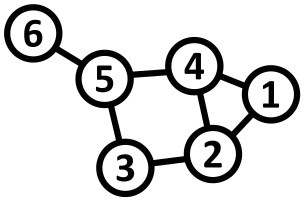
\includegraphics[keepaspectratio,alt={A graph with 6 vertices and edges (Image Credit: Wikipedia)}]{_main_files/fig/fig1.png}}
\caption{A graph with 6 vertices and edges \emph{(Image Credit: Wikipedia)}}
\end{figure}

The objects are represented as points called \textbf{vertices} (or \textbf{nodes}), and the connections between them are called \textbf{edges}.
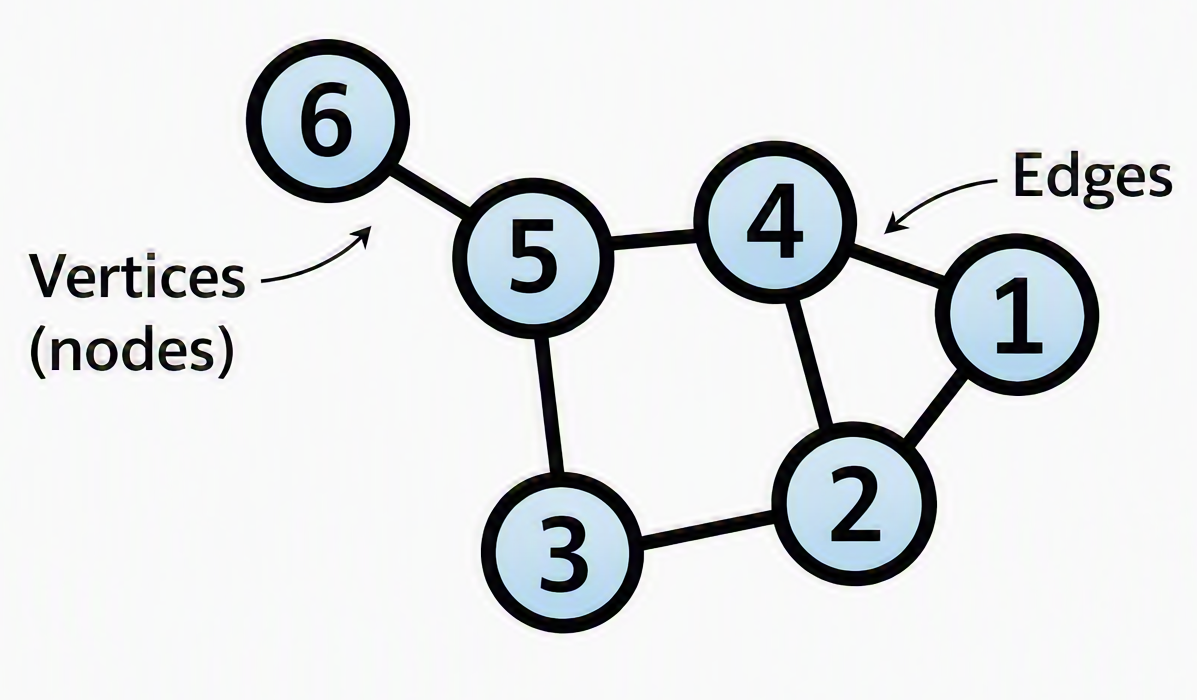
\includegraphics[width=0.5\linewidth,height=\textheight,keepaspectratio]{_main_files/fig/fig 2.png}

Graphs give us a unified mathematical language to represent networks. Whether we are analyzing social networks, computer communication grids, or transit maps, graph theory provides the core framework to understand how systems are connected.

\begin{center}\rule{0.5\linewidth}{0.5pt}\end{center}

\section{Historical Foundations}\label{historical-foundations}

To appreciate graph theory, it helps to understand the historical puzzles that sparked its development.

\subsection{The Seven Bridges of Königsberg (1736)}\label{the-seven-bridges-of-kuxf6nigsberg-1736}

Graph theory was born in the Prussian city of Königsberg (now Kaliningrad, Russia). The city was divided by the Pregel River, creating two large islands connected to each other and to the mainland riverbanks by seven bridges.

\begin{figure}
\centering
\pandocbounded{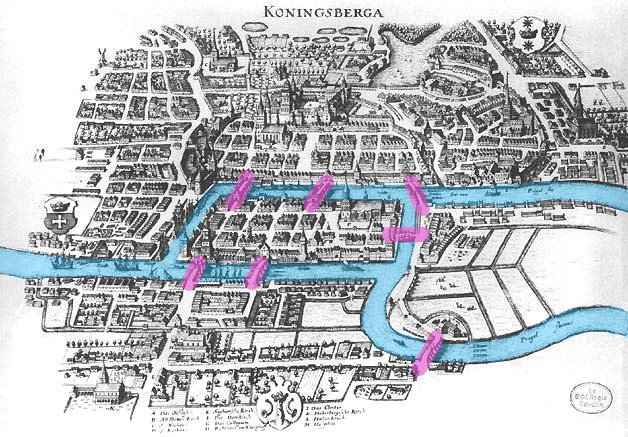
\includegraphics[keepaspectratio,alt={Image Source: Wikipedia}]{_main_files/fig/fig12.png}}
\caption{Image Source: Wikipedia}
\end{figure}

The citizens posed a classic recreational puzzle: \emph{Is it possible to take a walk through the city in such a way that you cross every single one of the seven bridges exactly once, and end up back where you started?}
\pandocbounded{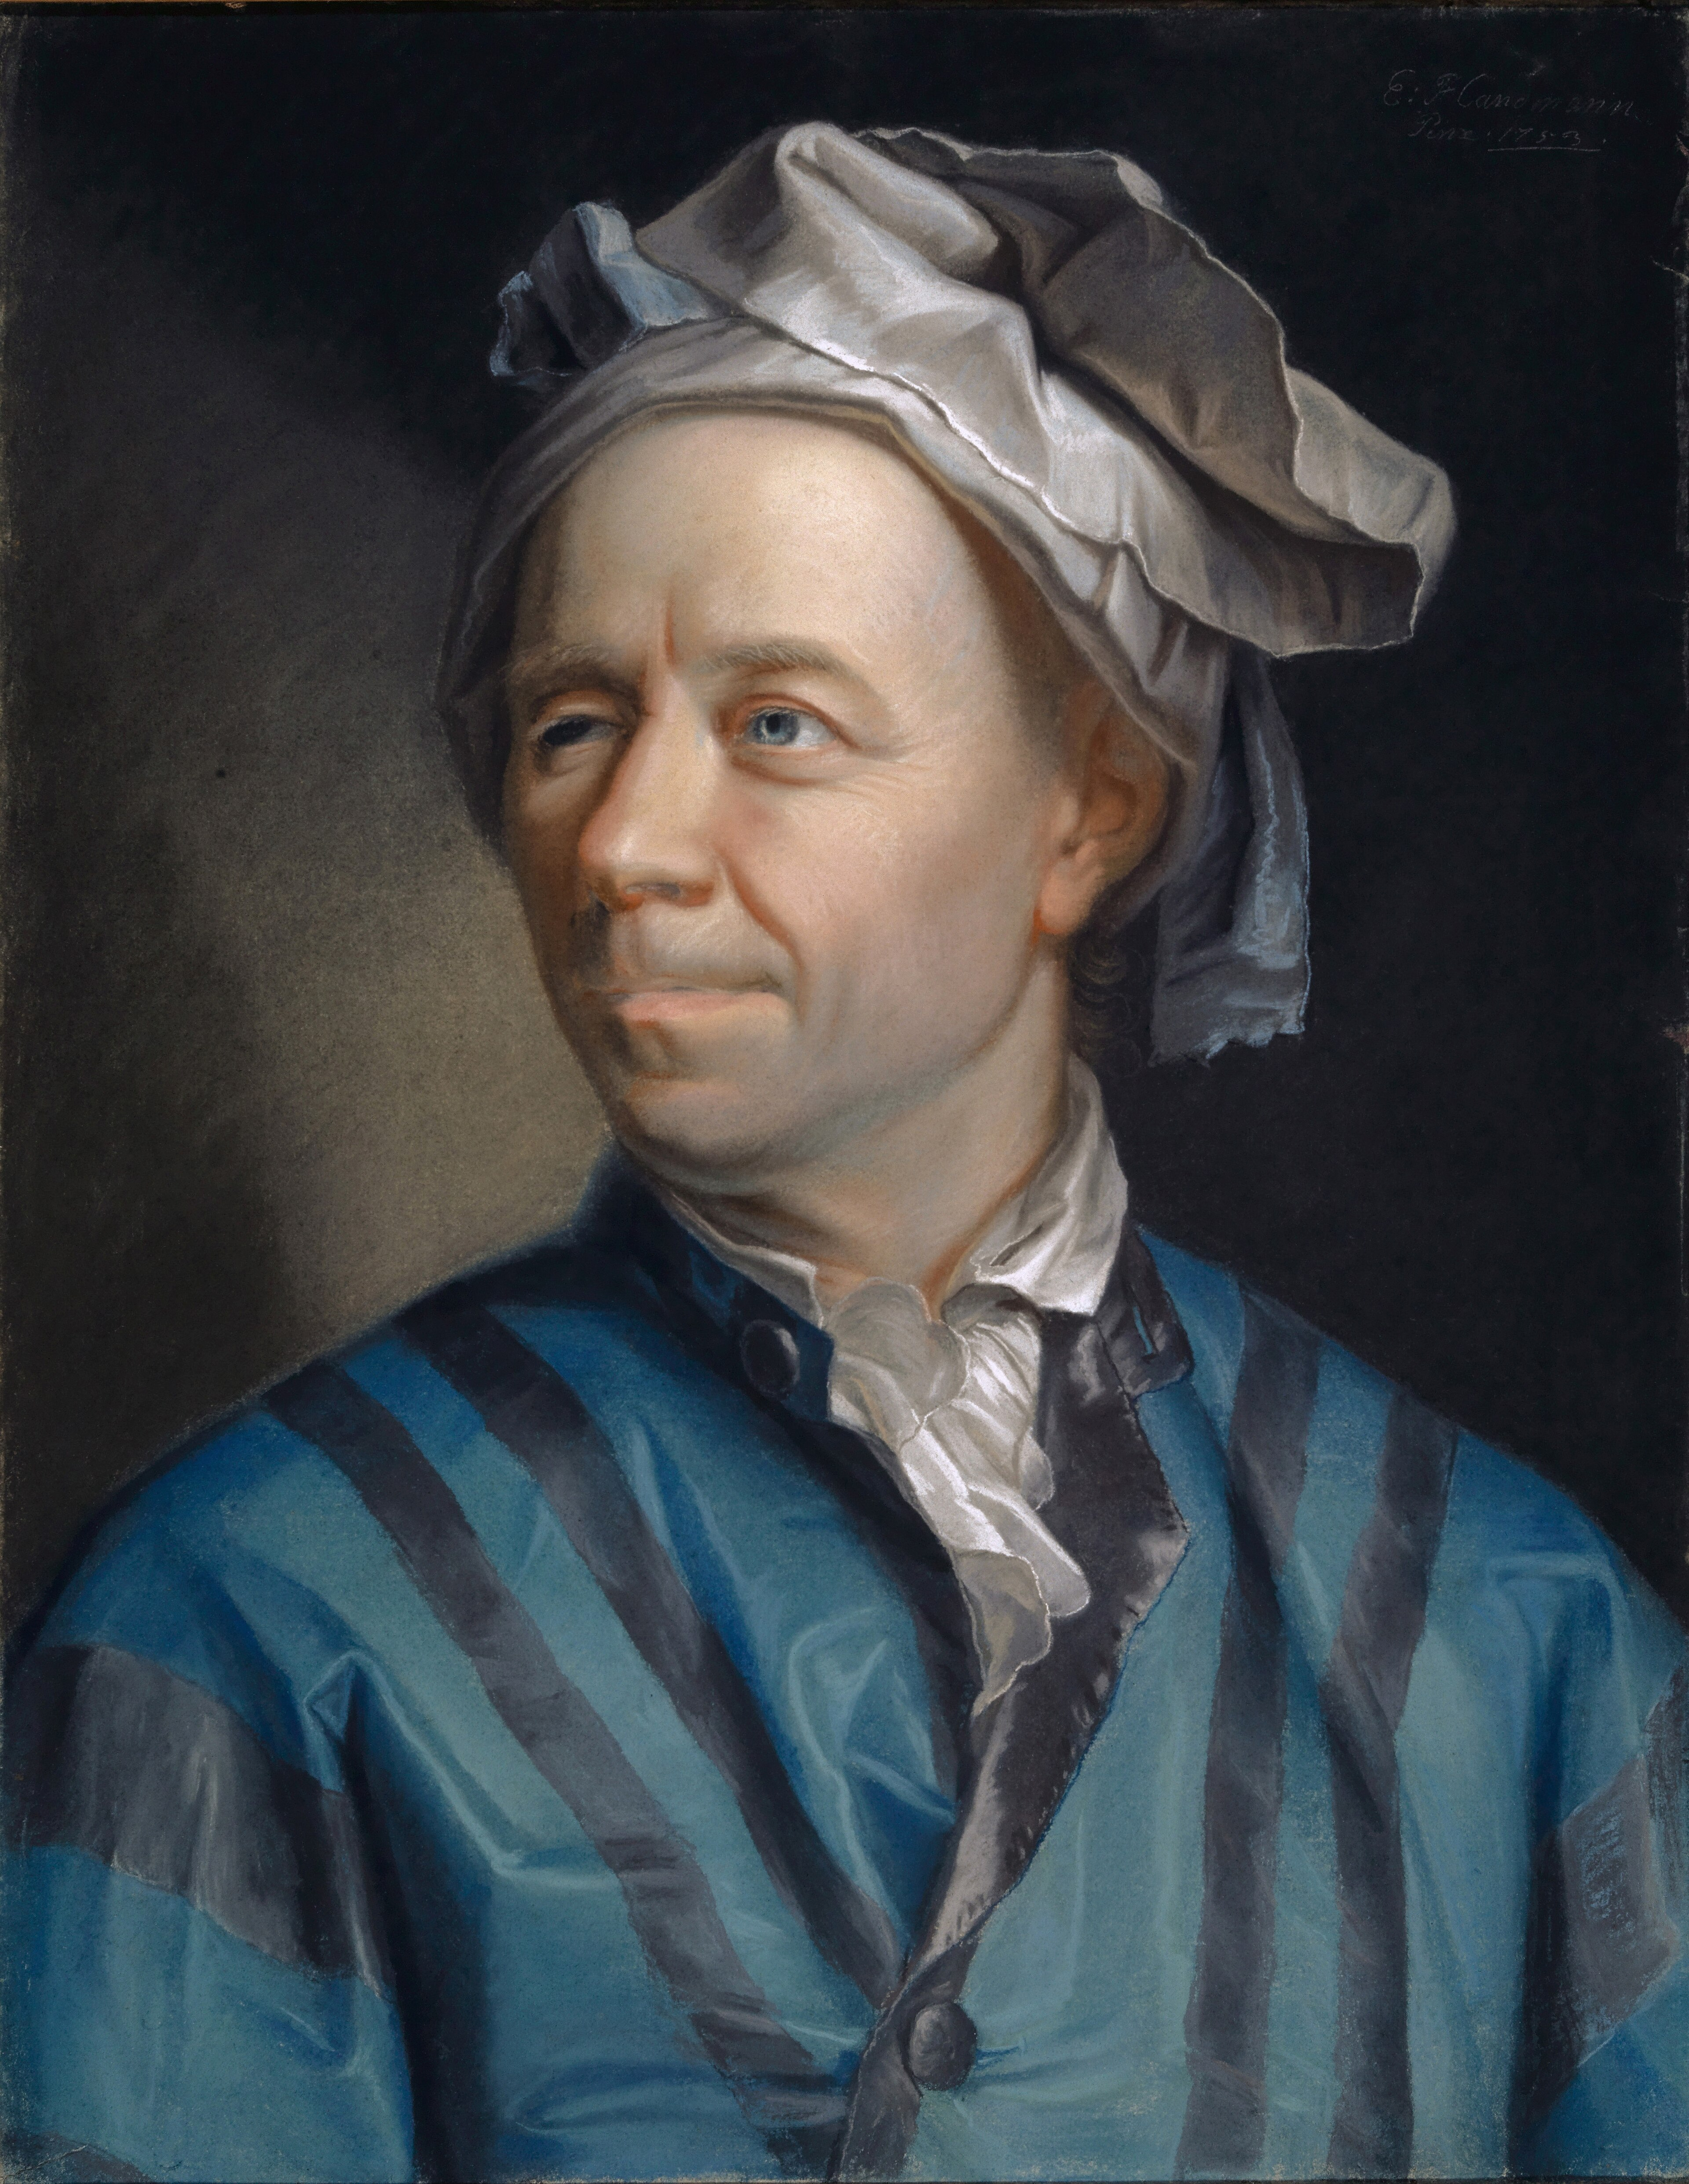
\includegraphics[keepaspectratio,alt={Leonhard Euler (Image Credit: Wikipedia)}]{_main_files/fig/fig14.jpg}}

In 1736, the Swiss mathematician \textbf{Leonhard Euler} solved this problem. He realized that the specific distances, land shapes, and physical geography did not matter; only the \textbf{connections} mattered. Euler simplified the map by replacing each landmass with a point (vertex) and each bridge with a line (edge).

\begin{figure}
\centering
\pandocbounded{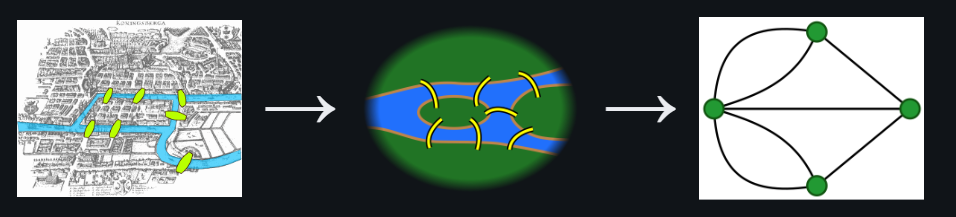
\includegraphics[keepaspectratio,alt={Image Credit: Wekipdea}]{_main_files/fig/fig 3.png}}
\caption{Image Credit: Wekipdea}
\end{figure}

By abstracting the geography into a mathematical structure, Euler proved that such a walk was impossible. In doing so, he laid the foundation for topology and graph theory.

\subsection{Hamilton's Icosian Game (1859)}\label{hamiltons-icosian-game-1859}

Over a century later, in 1859, Irish mathematician \textbf{Sir William Rowan Hamilton} created a commercial puzzle called the \emph{Icosian Game}.

\begin{figure}
\centering
\pandocbounded{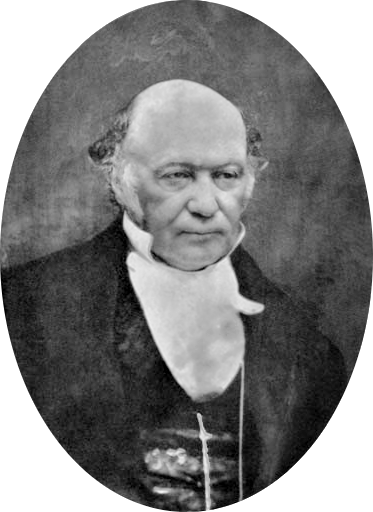
\includegraphics[keepaspectratio,alt={Porteat of Sir William Rowan Hamilton (Image Credit: Wikipedia)}]{_main_files/fig/fig13.png}}
\caption{Porteat of Sir William Rowan Hamilton (Image Credit: Wikipedia)}
\end{figure}

\begin{figure}
\centering
\pandocbounded{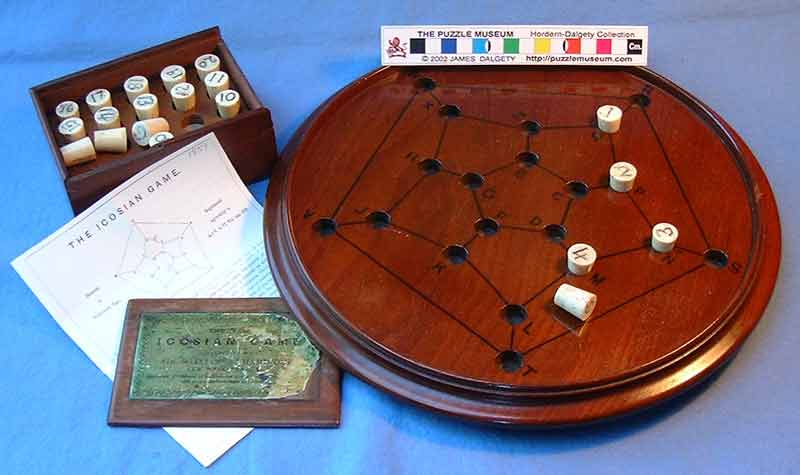
\includegraphics[keepaspectratio,alt={The Icosian Game(Image Credit: puzzlemuseum)}]{_main_files/a088af0fedcc82c2004161d5e82374b9a661a20b.jpg}}
\caption{The Icosian Game(Image Credit: puzzlemuseum)}
\end{figure}

The game used a solid wooden regular dodecahedron---a 12-faced polyhedron with 20 corners. Each of the 20 corners was labeled with the name of a famous world city. The objective was to find a route along the edges of the dodecahedron that visited \textbf{every city exactly once} and returned to the starting point.

While Euler's bridge problem focused on visiting every \emph{edge} once, Hamilton's game focused on visiting every \emph{vertex} once. These two historical problems led directly to two major areas of graph theory: \textbf{Eulerian paths} and \textbf{Hamiltonian cycles}.

\begin{center}\rule{0.5\linewidth}{0.5pt}\end{center}

\section{Modern Applications}\label{modern-applications}

Today, graph theory is an essential foundation for computer science, data analytics, and operational engineering.

\begin{itemize}
\item
  \textbf{Social Networks}: Platforms model users as vertices and friendships or followers as edges. Graph theory algorithms help identify tight-knit communities, influential users, and recommendation loops.
\item
  \textbf{Transportation Networks}: Airline routes, train networks, and road grids are modeled as graphs. GPS platforms rely on these models to compute optimal routes.
\item
  \textbf{The Web \& PageRank}: The World Wide Web is a massive graph where web pages are vertices and hyperlinks are directed edges. Early search engines transformed web searches by using graph structure to rank relevance based on link density.
\end{itemize}

\begin{center}\rule{0.5\linewidth}{0.5pt}\end{center}

\section{Formal Definitions and Basic Structures}\label{formal-definitions-and-basic-structures}

Let us establish the formal mathematical definitions used throughout graph theory.

\subsection{Mathematical Definition of a Graph}\label{mathematical-definition-of-a-graph}

A \textbf{graph} \(G\) is a pair \(G = (V, E)\), where:

\begin{itemize}
\tightlist
\item
  \(V\) is a non-empty set of \textbf{vertices} (or nodes).
\item
  \(E\) is a set of \textbf{edges}, where each edge \(e \in E\) is associated with an unordered pair of vertices \(\{u, v\} \subseteq V\).
\end{itemize}

If an edge \(e\) connects vertices \(u\) and \(v\), we write \(e = (u, v)\) or \(e = uv\). We say that \(e\) is \textbf{incident} with \(u\) and \(v\), and that \(u\) and \(v\) are \textbf{adjacent} (or neighbors).

\subsubsection{Example}\label{example}

\begin{example}
\protect\hypertarget{exm:unnamed-chunk-1}{}\label{exm:unnamed-chunk-1}

Consider a graph \(G = (V, E)\) defined by:

\begin{itemize}
\tightlist
\item
  \(V = \{v_1, v_2, v_3, v_4, v_5\}\)
\item
  \(E = \{e_1, e_2, e_3, e_4, e_5, e_6\}\) where:
\item
  \(e_1 = (v_1, v_2)\)
\item
  \(e_2 = (v_2, v_3)\)
\item
  \(e_3 = (v_3, v_4)\)
\item
  \(e_4 = (v_4, v_1)\)
\item
  \(e_5 = (v_1, v_3)\)
\item
  \(e_6 = (v_4, v_5)\)
\end{itemize}

\end{example}

\pandocbounded{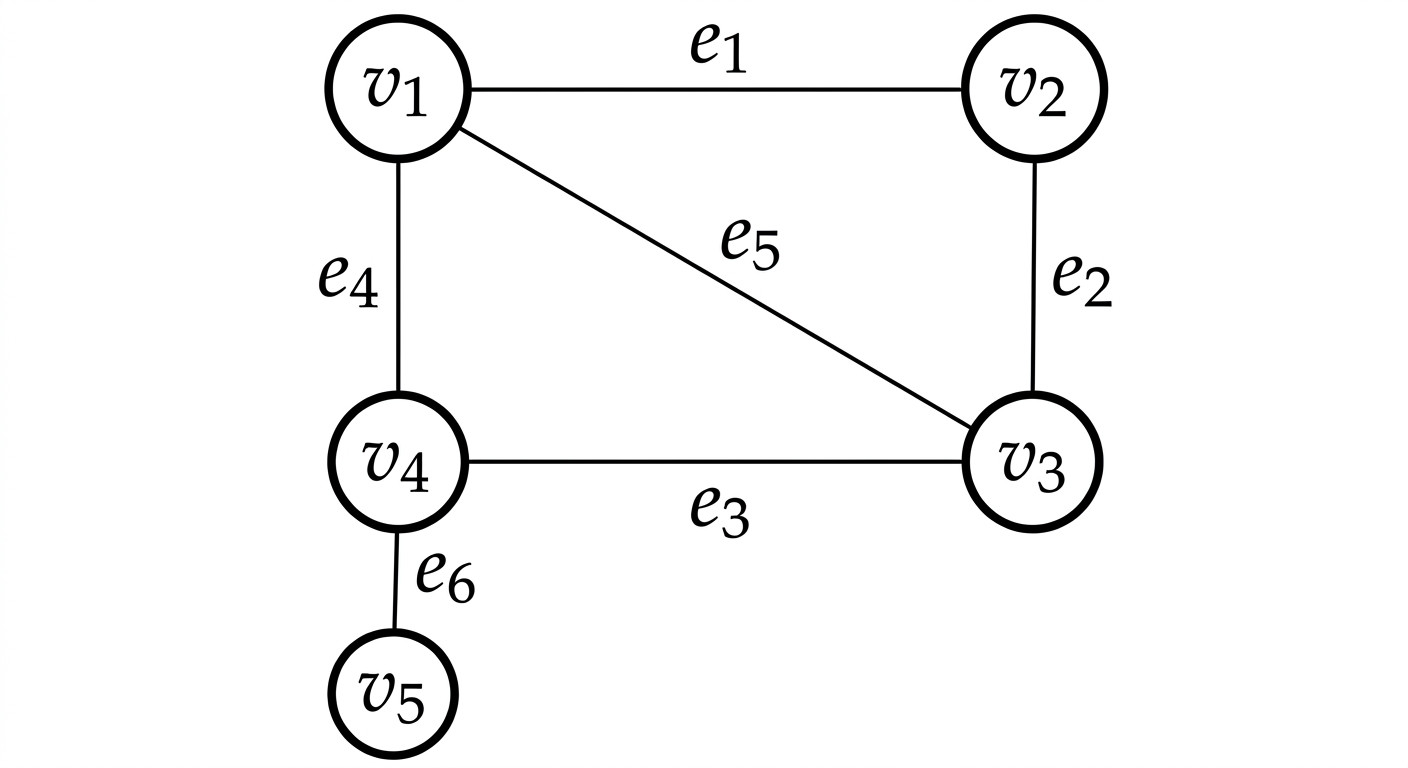
\includegraphics[keepaspectratio]{_main_files/fig/fig 4.jpeg}}

In this graph:

\begin{itemize}
\tightlist
\item
  \(v_1\) and \(v_3\) are adjacent because \(e_5 = (v_1, v_3)\) connects them.
\item
  \(v_2\) and \(v_5\) are \textbf{not} adjacent because there is no edge directly connecting them.
\end{itemize}

\begin{center}\rule{0.5\linewidth}{0.5pt}\end{center}

\subsection{Loops, Multiple Edges, and Simple Graphs}\label{loops-multiple-edges-and-simple-graphs}

Not all graphs are strictly constructed with single lines between distinct points.

\begin{itemize}
\tightlist
\item
  \textbf{Self-loop}: An edge that joins a vertex to itself (e.g., \(e = (v_1, v_1)\)).
\item
  \textbf{Multiple Edges (Parallel Edges)}: A collection of two or more edges that connect the exact same pair of distinct end vertices.
\item
  \textbf{Simple Graph}: A graph that contains \textbf{no self-loops and no multiple edges}.
\end{itemize}

\pandocbounded{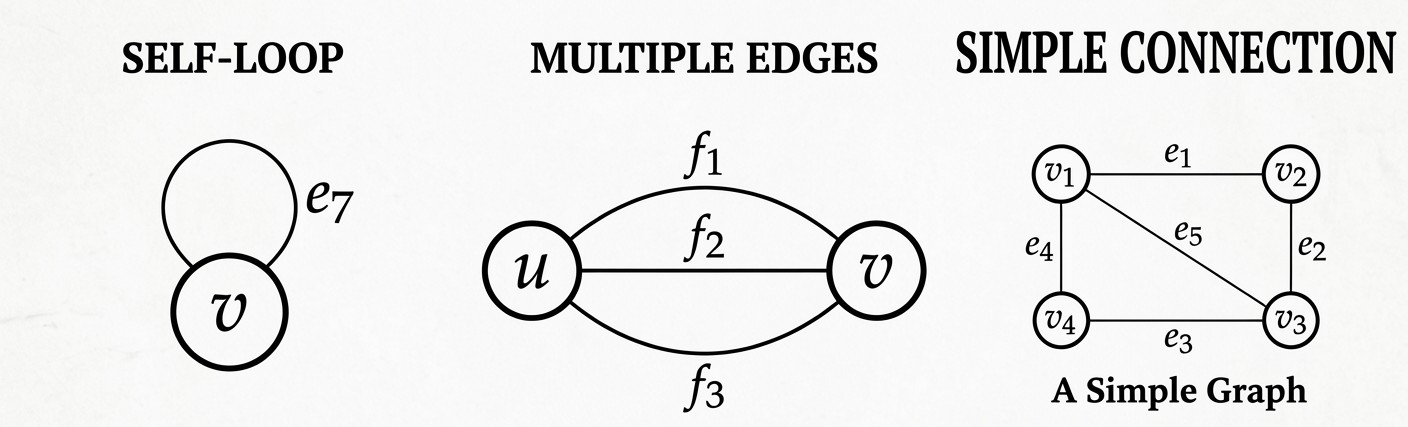
\includegraphics[keepaspectratio]{_main_files/fig/fig 5.jpeg}}

Unless specified otherwise, standard graph theory problems assume a graph is \textbf{simple}.

\begin{center}\rule{0.5\linewidth}{0.5pt}\end{center}

\section{Vertex Degrees and Handshaking}\label{vertex-degrees-and-handshaking}

\subsection{Vertex Degree}\label{vertex-degree}

The \textbf{degree} of a vertex \(v\), denoted by \(d(v)\), is the number of edges incident to \(v\). For simple graphs, it is equal to the number of neighbors connected to \(v\).

\emph{(Note: If a vertex has a self-loop, that loop contributes \(2\) to the vertex's degree, as it touches the vertex twice.)}

\subsubsection{Example}\label{example-1}

\begin{example}
\protect\hypertarget{exm:unnamed-chunk-2}{}\label{exm:unnamed-chunk-2}\pandocbounded{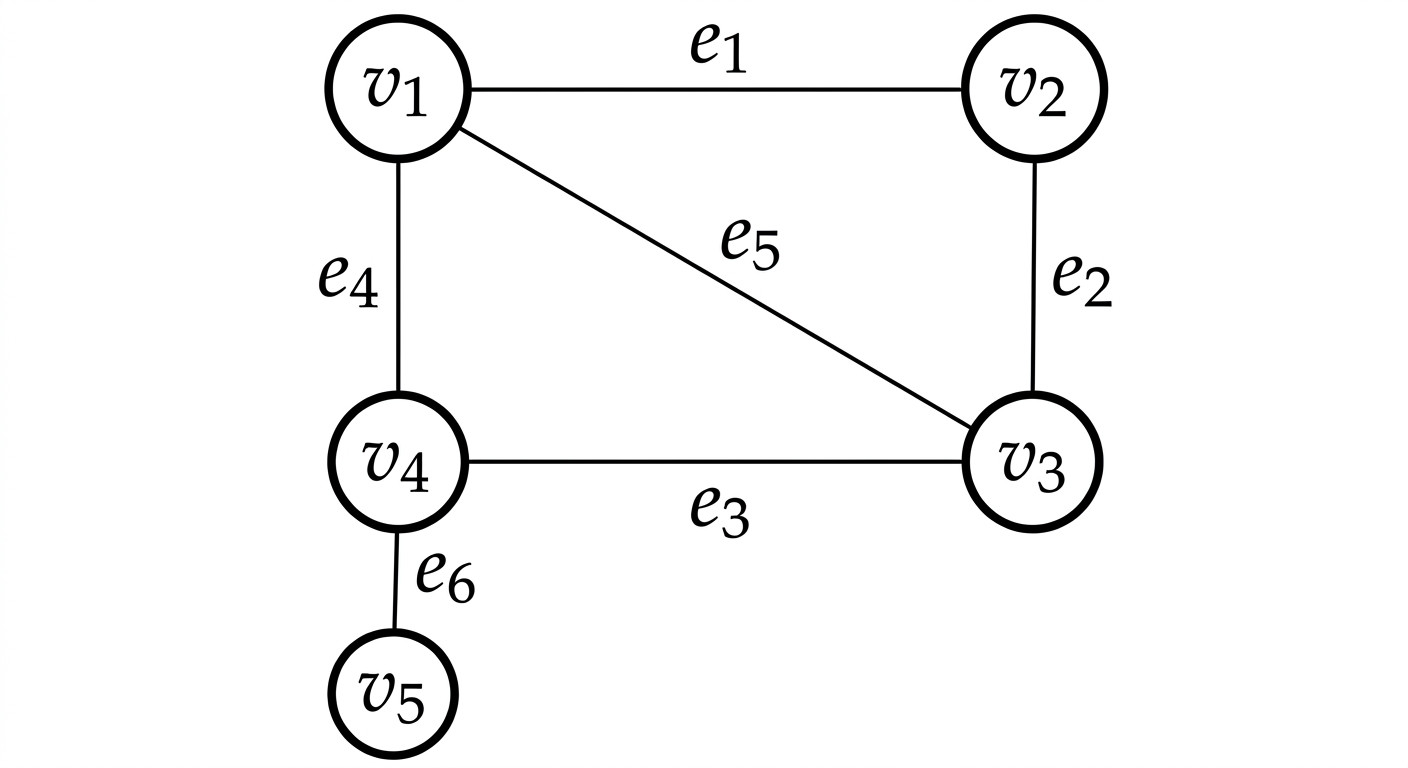
\includegraphics[keepaspectratio]{_main_files/fig/fig 4.jpeg}}
Using Example 1.1 above:

\begin{itemize}
\tightlist
\item
  \(d(v_1) = 3\) (connected by \(e_1, e_4, e_5\))
\item
  \(d(v_2) = 2\) (connected by \(e_1, e_2\))
\item
  \(d(v_3) = 3\) (connected by \(e_2, e_3, e_5\))
\item
  \(d(v_4) = 3\) (connected by \(e_3, e_4, e_6\))
\item
  \(d(v_5) = 1\) (connected by \(e_6\))
\end{itemize}

Summing all degrees: \(3 + 2 + 3 + 3 + 1 = 12\). Notice that the total number of edges \(\vert{}E\vert{}\) is \(6\). The sum of degrees (\(12\)) is exactly twice the number of edges (\(2 \times 6\)).
\end{example}

\begin{center}\rule{0.5\linewidth}{0.5pt}\end{center}

\subsection{The Handshaking Lemma}\label{the-handshaking-lemma}

This observation holds true for all graphs.

\begin{theorem}[Handshaking Lemma]
\protect\hypertarget{thm:unnamed-chunk-3}{}\label{thm:unnamed-chunk-3}Let \(G = (V, E)\) be any graph. Then the sum of the degrees of all vertices is equal to twice the number of edges:

\[\sum_{v \in V} d(v) = 2\vert{}E\vert{}\]
\end{theorem}

\begin{proof}
\emph{Intuition:}

Every edge \(e = (u, v)\) has two endpoints. When we count the degree of vertex \(u\), edge \(e\) contributes \(1\). When we count the degree of vertex \(v\), edge \(e\) contributes \(1\) again. Therefore, every edge contributes exactly \(2\) to the sum total of degrees in the graph.
\end{proof}

\begin{corollary}[The Parity of Odd-Degree Vertices]
\protect\hypertarget{cor:unnamed-chunk-5}{}\label{cor:unnamed-chunk-5}In any graph \(G\), the number of vertices that have an \textbf{odd degree} must be \textbf{even}.
\end{corollary}

\begin{proof}
Partition the vertex set \(V\) into two subsets: \(V_{\text{even}}\) (vertices with even degree) and \(V_{\text{odd}}\) (vertices with odd degree).

\[\sum_{v \in V} d(v) = \sum_{v \in V_{\text{even}}} d(v) + \sum_{v \in V_{\text{odd}}} d(v) = 2\vert{}E\vert{}\]

\begin{enumerate}
\def\labelenumi{\arabic{enumi}.}
\tightlist
\item
  The total sum \(2\vert{}E\vert{}\) is always an even integer.
\item
  The sum \(\sum_{v \in V_{\text{even}}} d(v)\) is a sum of even integers, so it must be even.
\item
  For the equation to balance, the sum \(\sum_{v \in V_{\text{odd}}} d(v)\) must also be \textbf{even}.
\item
  A sum of odd integers is even if and only if there is an \textbf{even number} of odd integers.
\end{enumerate}

Thus, the number of vertices with odd degree is always even.
\end{proof}

\begin{center}\rule{0.5\linewidth}{0.5pt}\end{center}

\section{Special Classes of Graphs}\label{special-classes-of-graphs}

Certain graph structures appear frequently throughout graph theory and computer science applications.

\subsection{\texorpdfstring{Complete Graphs (\(K_n\))}{Complete Graphs (K\_n)}}\label{complete-graphs-k_n}

\begin{definition}
\protect\hypertarget{def:unnamed-chunk-7}{}\label{def:unnamed-chunk-7}A \textbf{complete graph} on \(n\) vertices, denoted by \(K_n\), is a simple graph in which every pair of distinct vertices is connected by an edge.
\end{definition}

\begin{figure}
\centering
\pandocbounded{\includesvg[keepaspectratio]{_main_files/e11921f4d6ef553c24f07699de628ed8e56dfffb.svg}}
\caption{Complete graphs: wolfram math world}
\end{figure}

\begin{itemize}
\tightlist
\item
  \textbf{Number of Edges in \(K_n\)}:
  To find the total number of edges, we count how many ways we can pick a pair of vertices from \(n\) available vertices:
\end{itemize}

\[\vert{}E\vert{} = \binom{n}{2} = \frac{n(n - 1)}{2}\]

\subsection{Regular Graphs}\label{regular-graphs}

\begin{definition}
\protect\hypertarget{def:unnamed-chunk-8}{}\label{def:unnamed-chunk-8}A graph is \textbf{\(k\)-regular} if every vertex has the same degree \(k\).
\end{definition}

\begin{itemize}
\tightlist
\item
  In a \(k\)-regular graph with \(n\) vertices, \(\sum d(v) = n \cdot k\). By the Handshaking Lemma:
\end{itemize}

\[n \cdot k = 2\vert{}E\vert{} \implies \vert{}E\vert{} = \frac{n \cdot k}{2}\]

\begin{figure}
\centering
\pandocbounded{\includesvg[keepaspectratio]{_main_files/c9e340c32730dacf49f4c971ae9e354fbb74e5f5.svg}}
\caption{Examples of regular graphs(Image credit: Wolfarm math world)}
\end{figure}

\begin{itemize}
\tightlist
\item
  \textbf{Note}: A complete graph \(K_n\) is an \((n - 1)\)-regular graph.
\end{itemize}

\subsection{Bipartite Graphs}\label{bipartite-graphs}

\begin{definition}
\protect\hypertarget{def:unnamed-chunk-9}{}\label{def:unnamed-chunk-9}A graph \(G = (V, E)\) is \textbf{bipartite} if its vertex set \(V\) can be partitioned into two disjoint subsets, \(V_1\) and \(V_2\) (\(V = V_1 \cup V_2\) and \(V_1 \cap V_2 = \emptyset\)), such that every edge in \(E\) connects a vertex in \(V_1\) to a vertex in \(V_2\). No edges exist between two vertices within \(V_1\) or within \(V_2\).
\end{definition}

\begin{figure}
\centering
\pandocbounded{\includesvg[keepaspectratio]{_main_files/a270d025eae3b53f7b2528abd33c3bb7a72b1e50.svg}}
\caption{Image Credit: Mathworld Wolfarm}
\end{figure}

\subsubsection{\texorpdfstring{Complete Bipartite Graphs (\(K_{n_1, n_2}\))}{Complete Bipartite Graphs (K\_\{n\_1, n\_2\})}}\label{complete-bipartite-graphs-k_n_1-n_2}

A \textbf{complete bipartite graph} \(K_{n_1, n_2}\) is a bipartite graph where every vertex in \(V_1\) (with \(\vert{}V_1\vert{} = n_1\)) is connected to every vertex in \(V_2\) (with \(\vert{}V_2\vert{} = n_2\)).

\begin{itemize}
\tightlist
\item
  Total Vertices: \(\vert{}V\vert{} = n_1 + n_2\)
\item
  Total Edges: \(\vert{}E\vert{} = n_1 \cdot n_2\)
\end{itemize}

\subsubsection{Characterization Theorem of Bipartite Graphs}\label{characterization-theorem-of-bipartite-graphs}

How can we determine if a given graph is bipartite?

\begin{theorem}
\protect\hypertarget{thm:unnamed-chunk-10}{}\label{thm:unnamed-chunk-10}A graph \(G\) is bipartite \textbf{if and only if} it contains \textbf{no cycles of odd length}.
\end{theorem}

\pandocbounded{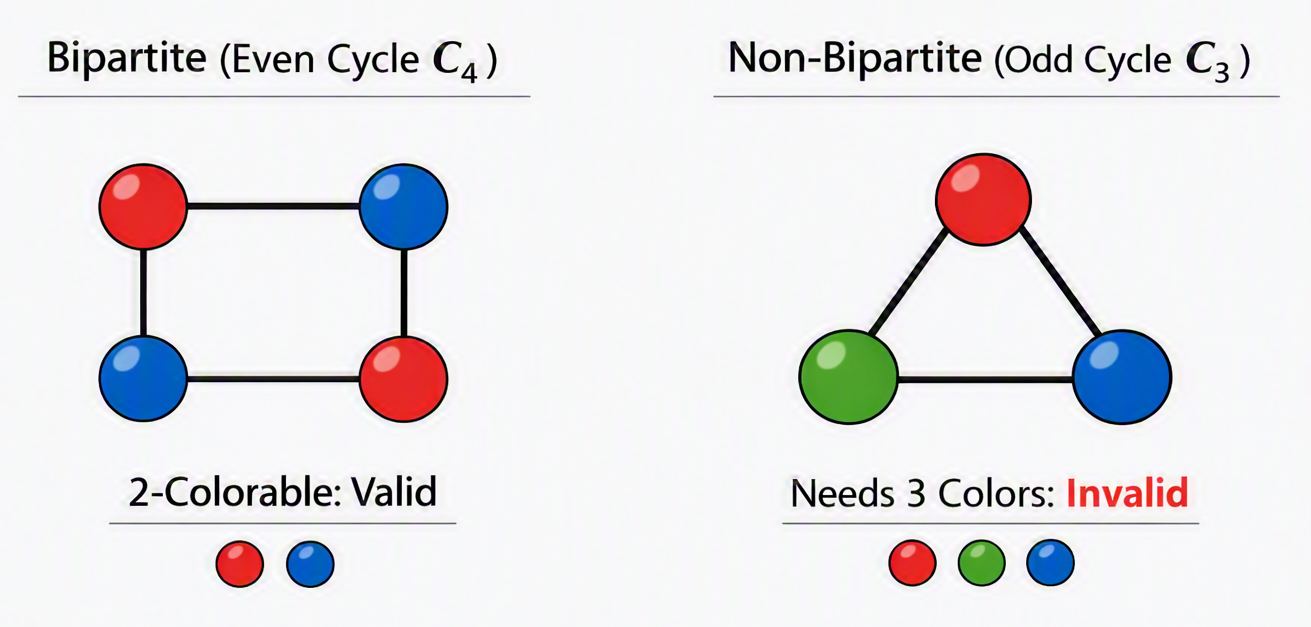
\includegraphics[keepaspectratio]{_main_files/fig/fig7.png}}

\begin{itemize}
\tightlist
\item
  If a graph contains a triangle (\(C_3\)), a pentagon (\(C_5\)), or any other cycle with an odd number of edges, it cannot be partitioned into two valid bipartite sets.
\end{itemize}

\begin{center}\rule{0.5\linewidth}{0.5pt}\end{center}

\section{Traversal Terminology: Walks, Trails, Paths, Circuits, and Cycles}\label{traversal-terminology-walks-trails-paths-circuits-and-cycles}

To navigate through a graph, we need clear definitions for moving along vertices and edges.

\pandocbounded{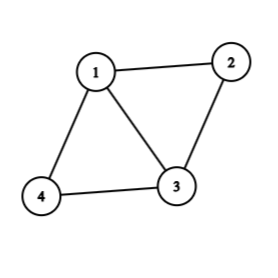
\includegraphics[keepaspectratio]{_main_files/fig/fig8.png}}

\subsection{Definitions}\label{definitions}

\begin{definition}
\protect\hypertarget{def:unnamed-chunk-11}{}\label{def:unnamed-chunk-11}\leavevmode

\begin{enumerate}
\def\labelenumi{\arabic{enumi}.}
\tightlist
\item
  \textbf{Walk}: A sequence of alternating vertices and edges, starting at vertex \(v_0\) and ending at \(v_k\): \(v_0, e_1, v_1, e_2, \dots, e_k, v_k\). Vertices and edges \textbf{may be repeated}.
\item
  \textbf{Trail}: A walk in which \textbf{no edge is repeated}. Vertices may still be repeated.
\item
  \textbf{Path}: A trail in which \textbf{no vertex is repeated}. (Consequently, no edge is repeated either).
\item
  \textbf{Closed Walk / Trail}: A walk or trail that starts and ends at the exact same vertex (\(v_0 = v_k\)).
\item
  \textbf{Circuit}: A \textbf{closed trail} (starts and ends at the same vertex, with no repeated edges).
\item
  \textbf{Cycle}: A \textbf{closed path} (starts and ends at the same vertex, with no repeated vertices other than the start and end).
\end{enumerate}

\end{definition}

\subsection{Summary Table}\label{summary-table}

{\def\LTcaptype{none} % do not increment counter
\begin{longtable}[]{@{}
  >{\raggedright\arraybackslash}p{(\linewidth - 6\tabcolsep) * \real{0.2500}}
  >{\raggedright\arraybackslash}p{(\linewidth - 6\tabcolsep) * \real{0.2500}}
  >{\raggedright\arraybackslash}p{(\linewidth - 6\tabcolsep) * \real{0.2500}}
  >{\raggedright\arraybackslash}p{(\linewidth - 6\tabcolsep) * \real{0.2500}}@{}}
\toprule\noalign{}
\begin{minipage}[b]{\linewidth}\raggedright
Structure
\end{minipage} & \begin{minipage}[b]{\linewidth}\raggedright
Repeated Vertices Allowed?
\end{minipage} & \begin{minipage}[b]{\linewidth}\raggedright
Repeated Edges Allowed?
\end{minipage} & \begin{minipage}[b]{\linewidth}\raggedright
Start and End at Same Vertex?
\end{minipage} \\
\midrule\noalign{}
\endhead
\bottomrule\noalign{}
\endlastfoot
\textbf{Walk} & Yes & Yes & Optional \\
\textbf{Trail} & Yes & \textbf{No} & Optional \\
\textbf{Path} & \textbf{No} & \textbf{No} & No \\
\textbf{Circuit} & Yes & \textbf{No} & \textbf{Yes} \\
\textbf{Cycle} & \textbf{No} (except start/end) & \textbf{No} & \textbf{Yes} \\
\end{longtable}
}

\begin{center}\rule{0.5\linewidth}{0.5pt}\end{center}

\section{Directed Graphs (Digraphs)}\label{directed-graphs-digraphs}

In many real-world networks, connections are one-way streets. For example, a web page may link to another, but that page might not link back.

\begin{definition}
\protect\hypertarget{def:unnamed-chunk-12}{}\label{def:unnamed-chunk-12}A \textbf{directed graph} (or \textbf{digraph}) consists of a vertex set \(V\) and an edge set \(E\) containing \textbf{ordered pairs} of vertices. An edge \(e = (u, v)\) goes \textbf{from \(u\) to \(v\)}.
\end{definition}

\pandocbounded{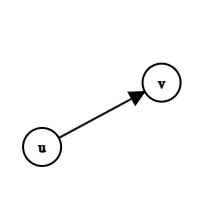
\includegraphics[keepaspectratio]{_main_files/fig/fig9.png}}

\subsection{In-Degree and Out-Degree}\label{in-degree-and-out-degree}

\begin{definition}
\protect\hypertarget{def:unnamed-chunk-13}{}\label{def:unnamed-chunk-13}Because edges have direction in a digraph, we split vertex degree into two separate counts:

\begin{itemize}
\tightlist
\item
  \textbf{In-degree (\(d_{\text{in}}(v)\))}: The number of directed edges coming \textbf{into} vertex \(v\).
\item
  \textbf{Out-degree (\(d_{\text{out}}(v)\))}: The number of directed edges going \textbf{out of} vertex \(v\).
\end{itemize}

\pandocbounded{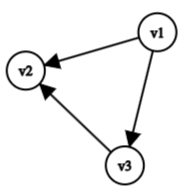
\includegraphics[keepaspectratio]{_main_files/fig/fig10.png}}
\end{definition}

In the example above:

\begin{itemize}
\tightlist
\item
  \(d_{\text{in}}(v_1) = 0\), \(d_{\text{out}}(v_1) = 2\)
\item
  \(d_{\text{in}}(v_2) = 2\), \(d_{\text{out}}(v_2) = 0\)
\item
  \(d_{\text{in}}(v_3) = 1\), \(d_{\text{out}}(v_3) = 1\)
\end{itemize}

\subsubsection{Handshaking Lemma for Directed Graphs}\label{handshaking-lemma-for-directed-graphs}

\begin{theorem}[Handshaking Lemma for Directed Graphs]
\protect\hypertarget{thm:unnamed-chunk-14}{}\label{thm:unnamed-chunk-14}In any directed graph, the sum of all in-degrees equals the sum of all out-degrees, which both equal the total number of directed edges:

\[\sum_{v \in V} d_{\text{in}}(v) = \sum_{v \in V} d_{\text{out}}(v) = \vert{}E\vert{}\]
\end{theorem}

\begin{center}\rule{0.5\linewidth}{0.5pt}\end{center}

\section{Chapter 1 Exercises}\label{chapter-1-exercises}

\begin{example}
\protect\hypertarget{exm:unnamed-chunk-15}{}\label{exm:unnamed-chunk-15}\leavevmode

\begin{enumerate}
\def\labelenumi{\arabic{enumi}.}
\tightlist
\item
  \textbf{Degree Calculations}: A simple graph has 8 vertices and 14 edges. If 4 vertices have degree 4, and 3 vertices have degree 3, what is the degree of the remaining vertex?
\item
  \textbf{Bipartite Verification}: Prove or disprove whether a single cycle graph \(C_6\) (a cycle with 6 vertices) is bipartite. What about \(C_7\)?
\item
  \textbf{Complete Graph Proof}: Use induction to show that the number of edges in a complete graph \(K_n\) is given by \(\frac{n(n-1)}{2}\).
\item
  \textbf{Handshaking Lemma}: Is it possible to construct a simple graph with 5 vertices such that their degrees are \(3, 3, 3, 2, 1\)? Explain using the Handshaking Lemma.
\end{enumerate}

\end{example}

\chapter{Graph Types, Operations \& Representations}\label{graph-types-operations-representations}

\section{Graph Isomorphism and Counting}\label{graph-isomorphism-and-counting}

When we draw graphs, we often place vertices in different positions on a page or bend edges around each other. However, graph theory focuses on connectivity rather than spatial layout. Two graphs that look entirely different on paper might actually share the exact same structural connections.

\subsection{Graph Isomorphism}\label{graph-isomorphism}

Two graphs \(G_1 = (V_1, E_1)\) and \(G_2 = (V_2, E_2)\) are \textbf{isomorphic} (denoted \(G_1 \cong G_2\)) if there exists a bijection (a one-to-one and onto mapping) \(f: V_1 \to V_2\) such that any two vertices \(u, v \in V_1\) are adjacent in \(G_1\) \textbf{if and only if} \(f(u)\) and \(f(v)\) are adjacent in \(G_2\).

In simple terms, an isomorphism is a relabeling of vertices that preserves all connections and non-connections.

\pandocbounded{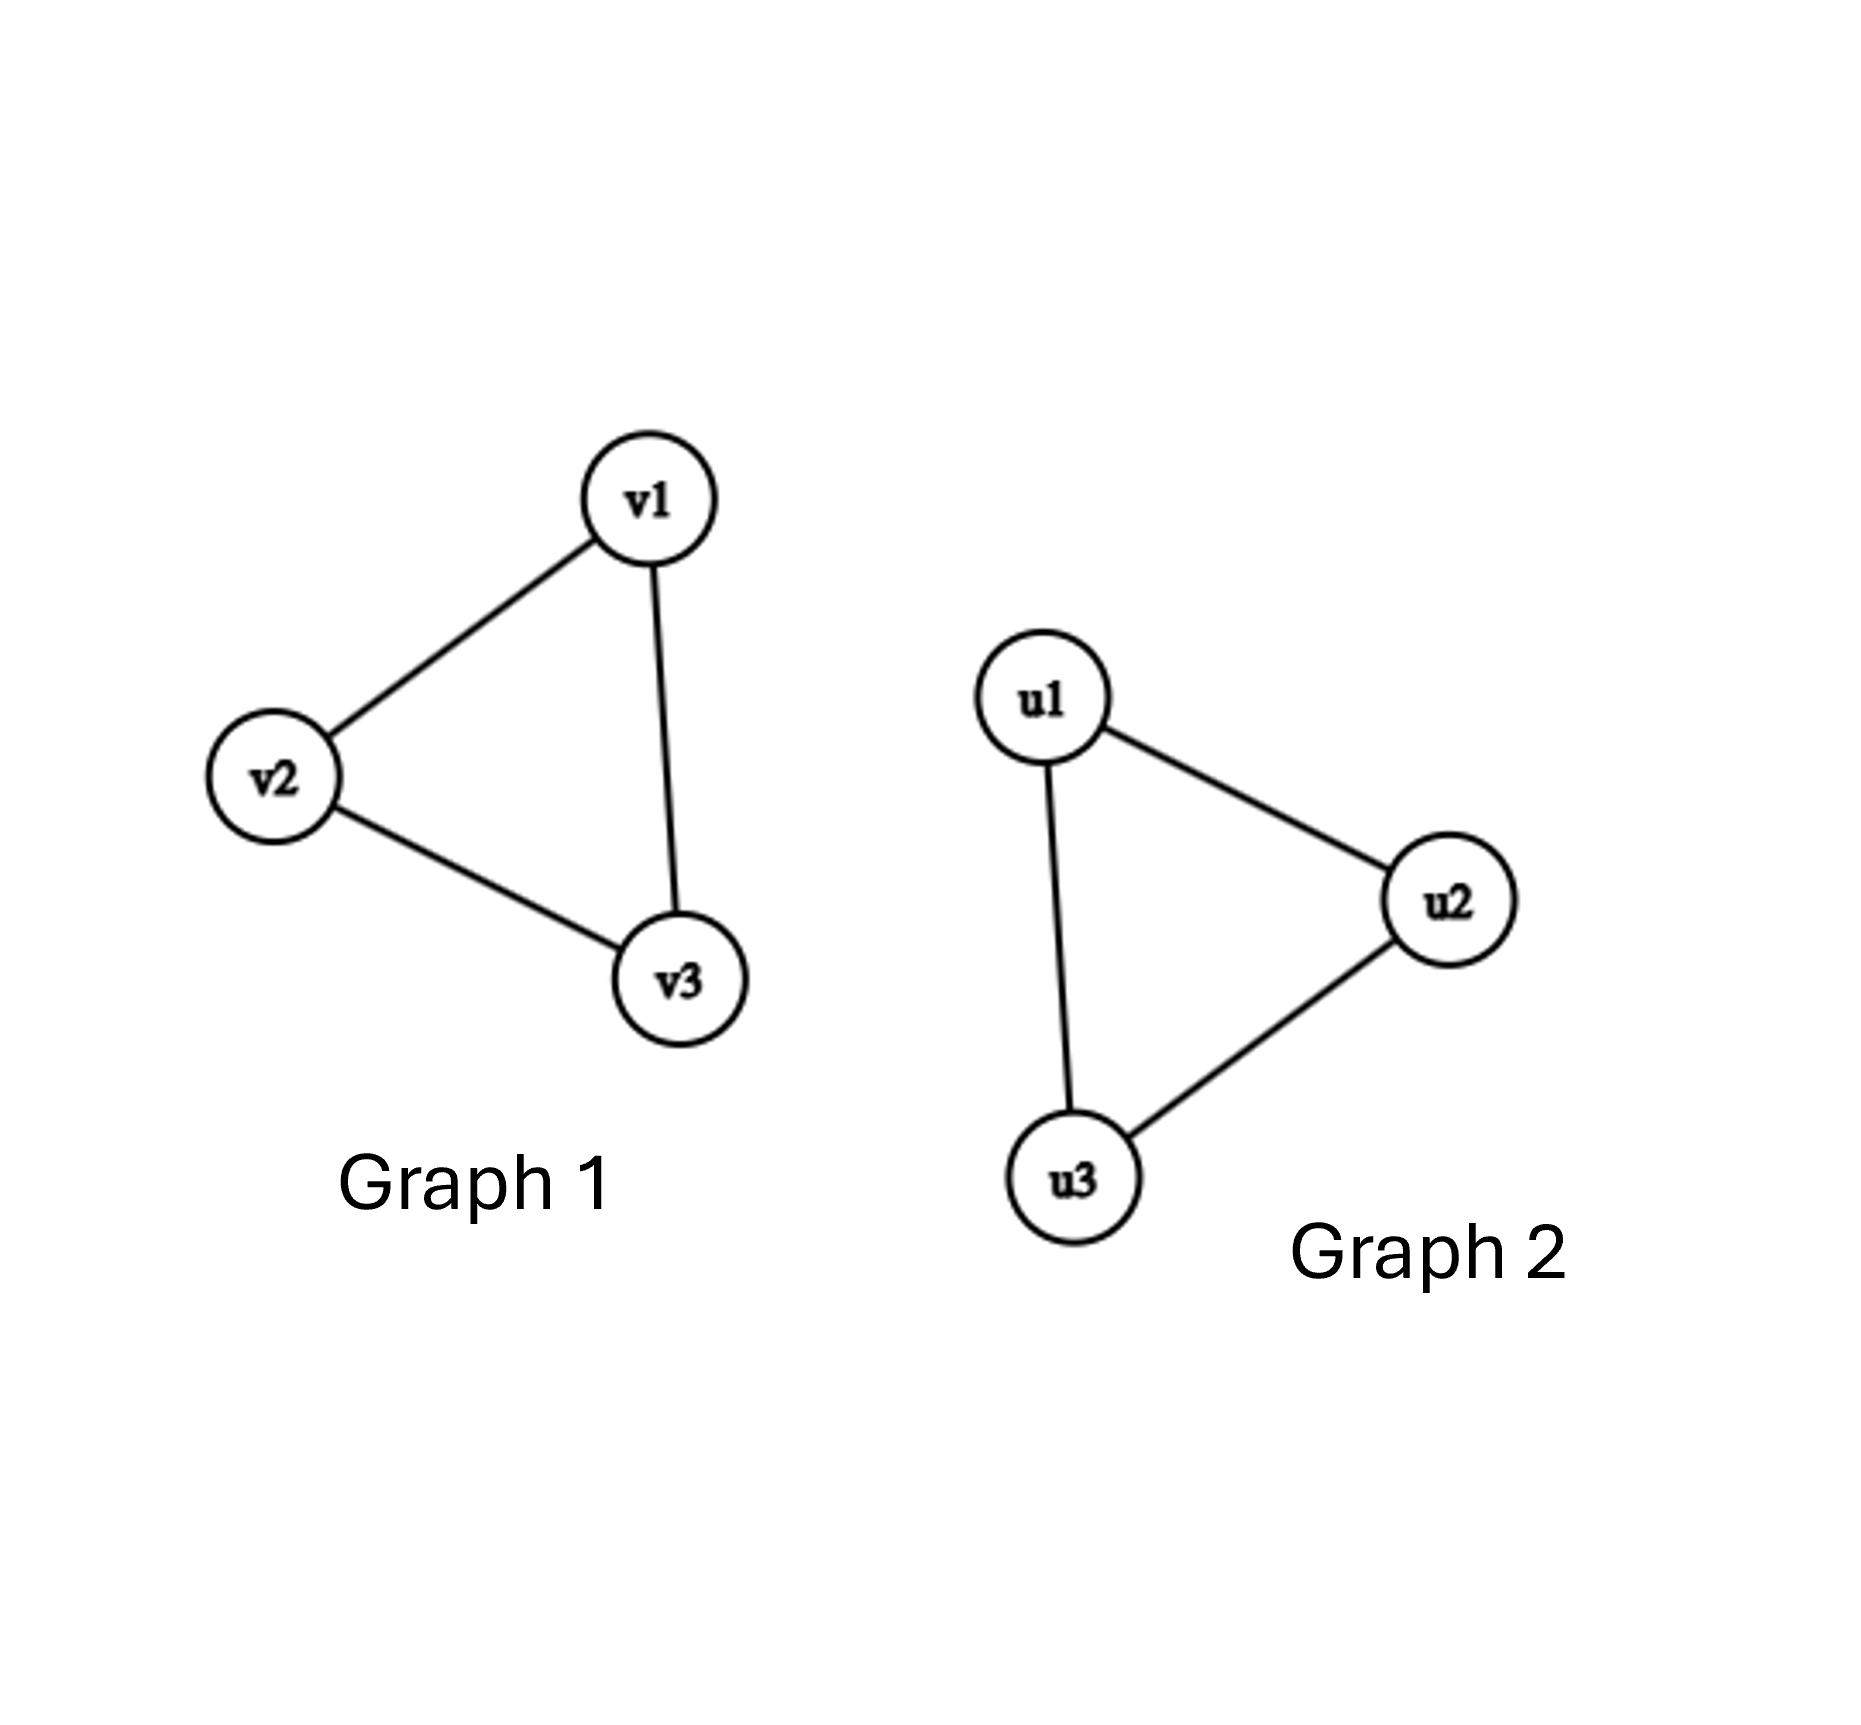
\includegraphics[keepaspectratio]{_main_files/fig/fig11.png}}

\subsubsection{Invariants Under Isomorphism}\label{invariants-under-isomorphism}

If two graphs are isomorphic, they must share structural properties called \textbf{graph invariants}. If any of these properties differ, the graphs cannot be isomorphic:

\begin{enumerate}
\def\labelenumi{\arabic{enumi}.}
\item
  The same number of vertices (\(\vert{}V_1\vert{} = \vert{}V_2\vert{}\)).
\item
  The same number of edges (\(\vert{}E_1\vert{} = \vert{}E_2\vert{}\)).
\item
  The exact same degree sequence (the degrees of all vertices listed in non-increasing order).
\item
  The same subgraphs, cycles of specific lengths, and structural properties.
\end{enumerate}

\subsubsection{Example}\label{example-2}

\begin{example}
\protect\hypertarget{exm:unnamed-chunk-16}{}\label{exm:unnamed-chunk-16}Consider two graphs \(G_1\) and \(G_2\) with \(V_1 = \{1, 2, 3, 4\}\) and \(V_2 = \{a, b, c, d\}\).

\begin{itemize}
\tightlist
\item
  \(E_1 = \{(1,2), (2,3), (3,4), (4,1)\}\) (a 4-cycle \(C_4\))
\item
  \(E_2 = \{(a,b), (b,c), (c,d), (d,a)\}\) (a 4-cycle \(C_4\))
\end{itemize}

We can define the bijection \(f(1)=a, f(2)=b, f(3)=c, f(4)=d\). Since every edge \((i, j) \in E_1\) corresponds to \((f(i), f(j)) \in E_2\), \(G_1 \cong G_2\).
\end{example}

\emph{(Note: While checking if two graphs are isomorphic is easy once the mapping \(f\) is given, determining whether a mapping exists for two arbitrary large graphs is a famously difficult problem in computer science, known as the Graph Isomorphism problem.)}

\begin{center}\rule{0.5\linewidth}{0.5pt}\end{center}

\subsection{Counting Simple Graphs}\label{counting-simple-graphs}

How many distinct graphs can we form given a fixed set of \(n\) vertices?

\begin{enumerate}
\def\labelenumi{\arabic{enumi}.}
\tightlist
\item
  \textbf{Maximum Edges in a Simple Graph}:
  In a simple graph with \(n\) vertices, every vertex can connect to at most \(n-1\) other vertices. Counting all pairs gives:
\end{enumerate}

\[\text{Maximum Edges} = \binom{n}{2} = \frac{n(n-1)}{2}\]

\begin{enumerate}
\def\labelenumi{\arabic{enumi}.}
\setcounter{enumi}{1}
\tightlist
\item
  \textbf{Total Labeled Graphs}:
  If the \(n\) vertices are labeled (distinct), each of the \(\frac{n(n-1)}{2}\) potential edges can either be present (\(1\)) or absent (\(0\)). Thus, the total number of labeled simple graphs on \(n\) vertices is:
\end{enumerate}

\[N_{\text{labeled}} = 2^{\frac{n(n-1)}{2}}\]

\begin{enumerate}
\def\labelenumi{\arabic{enumi}.}
\setcounter{enumi}{2}
\tightlist
\item
  \textbf{Unlabeled (Non-Isomorphic) Graphs}:
  If vertices are indistinguishable, we count non-isomorphic equivalence classes \(T_n\). Since there are at most \(n!\) ways to permute the labels of \(n\) vertices, \(T_n\) satisfies the bounds:
\end{enumerate}

\[\frac{2^{n(n-1)/2}}{n!} \le T_n \le 2^{n(n-1)/2}\]

\begin{center}\rule{0.5\linewidth}{0.5pt}\end{center}

\section{Graph Transformations and Operations}\label{graph-transformations-and-operations}

We can construct new graphs from existing ones using structural transformations.

\subsection{\texorpdfstring{The Complement Graph (\(\overline{G}\))}{The Complement Graph (\textbackslash overline\{G\})}}\label{the-complement-graph-overlineg}

Given a simple graph \(G = (V, E)\), its \textbf{complement} \(\overline{G} = (V, E')\) shares the exact same vertex set \(V\), but its edge set \(E'\) consists of all edges that are \textbf{missing} from \(G\).

\[e = (u, v) \in E' \iff e = (u, v) \notin E \quad \text{for } u \neq v\]

{\def\LTcaptype{none} % do not increment counter
\begin{longtable}[]{@{}cc@{}}
\toprule\noalign{}
Original Graph \(G\) & Complement Graph \(\bar{G}\) \\
\midrule\noalign{}
\endhead
\bottomrule\noalign{}
\endlastfoot
\pandocbounded{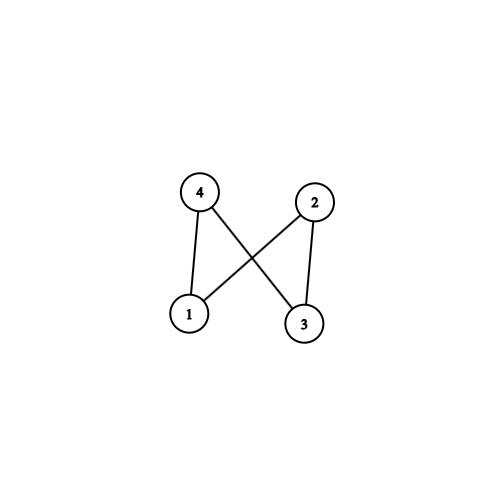
\includegraphics[keepaspectratio]{_main_files/fig/fig14.png}} & \pandocbounded{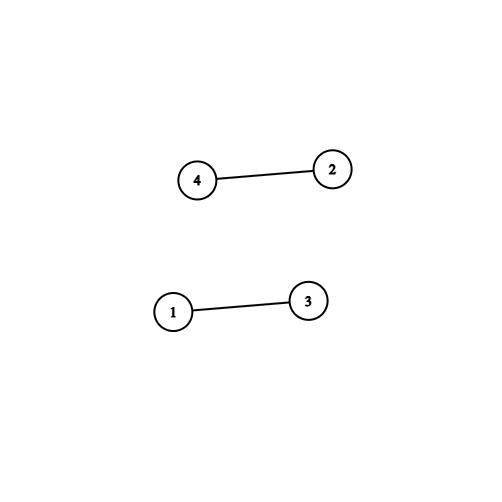
\includegraphics[keepaspectratio]{_main_files/fig/fig15.png}} \\
\end{longtable}
}

\subsubsection{Properties of Complements}\label{properties-of-complements}

\begin{itemize}
\item
  \(G \cup \overline{G} = K_n\) (The union of \(G\) and \(\overline{G}\) forms the complete graph \(K_n\)).
\item
  \(\vert{}E(G)\vert{} + \vert{}E(\overline{G})\vert{} = \frac{n(n-1)}{2}\).
\item
  A graph \(G\) is called \textbf{self-complementary} if \(G \cong \overline{G}\).
\end{itemize}

\begin{center}\rule{0.5\linewidth}{0.5pt}\end{center}

\subsection{\texorpdfstring{The Line Graph (\(L(G)\))}{The Line Graph (L(G))}}\label{the-line-graph-lg}

The \textbf{line graph} \(L(G)\) flips the structural roles of vertices and edges:

\begin{itemize}
\item
  Every \textbf{vertex} in \(L(G)\) represents an \textbf{edge} in \(G\).
\item
  Two vertices in \(L(G)\) are adjacent \textbf{if and only if} their corresponding edges in \(G\) share a common endpoint.
\end{itemize}

{\def\LTcaptype{none} % do not increment counter
\begin{longtable}[]{@{}ccc@{}}
\toprule\noalign{}
Original Graph \(G\) & & Line Graph \(L(G)\) \\
\midrule\noalign{}
\endhead
\bottomrule\noalign{}
\endlastfoot
\pandocbounded{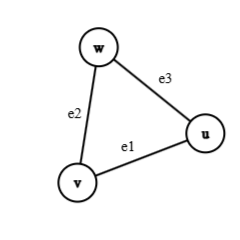
\includegraphics[keepaspectratio]{_main_files/fig/fig19.png}} & \pandocbounded{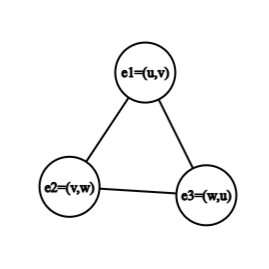
\includegraphics[keepaspectratio]{_main_files/fig/fig21.png}} & \pandocbounded{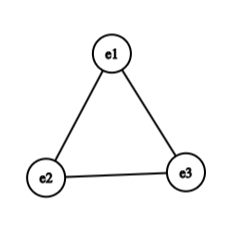
\includegraphics[keepaspectratio]{_main_files/fig/fig20.png}} \\
\end{longtable}
}

\subsubsection{Example}\label{example-3}

\begin{example}
\protect\hypertarget{exm:unnamed-chunk-17}{}\label{exm:unnamed-chunk-17}

Let \(G = P_4\), a path graph with 4 vertices \(\{1, 2, 3, 4\}\) and 3 edges \(e_1=(1,2), e_2=(2,3), e_3=(3,4)\).

\begin{itemize}
\tightlist
\item
  In \(L(G)\), the vertices are \(\{e_1, e_2, e_3\}\).
\item
  Edge \(e_1\) shares vertex \(2\) with \(e_2\), so \((e_1, e_2)\) is an edge in \(L(G)\).
\item
  Edge \(e_2\) shares vertex \(3\) with \(e_3\), so \((e_2, e_3)\) is an edge in \(L(G)\).
\item
  Edge \(e_1\) and \(e_3\) share no vertices, so there is no edge between \(e_1\) and \(e_3\).
\item
  Thus, \(L(P_4) \cong P_3\).
\end{itemize}

\end{example}

\begin{center}\rule{0.5\linewidth}{0.5pt}\end{center}

\section{Eulerian and Hamiltonian Graphs}\label{eulerian-and-hamiltonian-graphs}

Two classic traversal problems focus on traversing either every \textbf{edge} or every \textbf{vertex} of a graph.

\subsection{Eulerian Graphs (Edge Traversals)}\label{eulerian-graphs-edge-traversals}

\begin{itemize}
\item
  \textbf{Eulerian Trail}: A trail that visits every \textbf{edge} of \(G\) exactly once.
\item
  \textbf{Eulerian Tour (or Circuit)}: A closed Eulerian trail that starts and ends at the same vertex.
\item
  \textbf{Eulerian Graph}: A graph that contains an Eulerian tour.
\end{itemize}

\begin{figure}
\centering
\pandocbounded{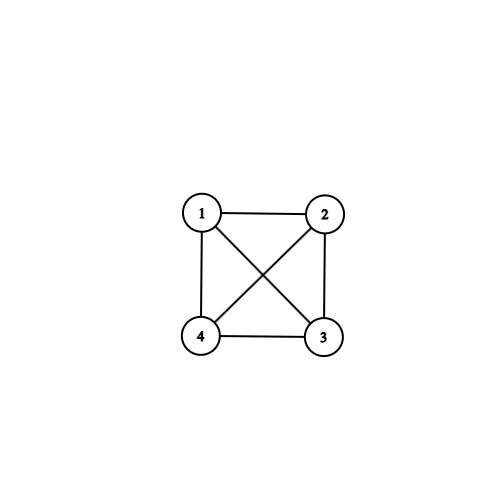
\includegraphics[keepaspectratio,alt={Euler Cricuit}]{_main_files/fig/fig16.png}}
\caption{Euler Cricuit}
\end{figure}

Sequence: 1 \(\rightarrow\) 2 \(\rightarrow\) 3 \(\rightarrow\) 4 \(\rightarrow\) 1 \(\rightarrow\) 3 \(\rightarrow\) 4 \(\rightarrow\) 2 \(\rightarrow\) 1

\subsubsection{Euler's Theorem}\label{eulers-theorem}

\begin{theorem}
\protect\hypertarget{thm:unnamed-chunk-18}{}\label{thm:unnamed-chunk-18}A connected graph \(G\) contains an Eulerian tour \textbf{if and only if} every vertex in \(G\) has an \textbf{even degree}.
\end{theorem}

\begin{theorem}[Eulerian Trail]
\protect\hypertarget{thm:unnamed-chunk-19}{}\label{thm:unnamed-chunk-19}A connected graph \(G\) contains an open Eulerian trail (starting at \(u\) and ending at \(v\), where \(u \neq v\)) \textbf{if and only if} \(u\) and \(v\) have \textbf{odd degrees}, and all other vertices have \textbf{even degrees}.
\end{theorem}

\begin{center}\rule{0.5\linewidth}{0.5pt}\end{center}

\subsection{Hamiltonian Graphs (Vertex Traversals)}\label{hamiltonian-graphs-vertex-traversals}

\begin{definition}
\protect\hypertarget{def:unnamed-chunk-20}{}\label{def:unnamed-chunk-20}\leavevmode

\begin{itemize}
\item
  \textbf{Hamiltonian Path}: A path that visits every \textbf{vertex} of \(G\) exactly once.
\item
  \textbf{Hamiltonian Cycle}: A closed cycle that visits every \textbf{vertex} of \(G\) exactly once.
\item
  \textbf{Hamiltonian Graph}: A graph that contains a Hamiltonian cycle.
\end{itemize}

\end{definition}

\begin{figure}
\centering
\pandocbounded{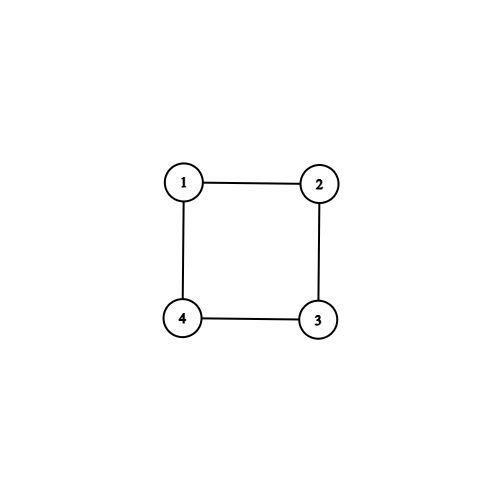
\includegraphics[keepaspectratio,alt={Hamiltonian Cycle}]{_main_files/fig/fig17.png}}
\caption{Hamiltonian Cycle}
\end{figure}

Sequence: 1 \(\rightarrow\) 2 \(\rightarrow\) 3 \(\rightarrow\) 4 \(\rightarrow\) 1

\subsubsection{Eulerian vs.~Hamiltonian Summary}\label{eulerian-vs.-hamiltonian-summary}

{\def\LTcaptype{none} % do not increment counter
\begin{longtable}[]{@{}
  >{\raggedright\arraybackslash}p{(\linewidth - 4\tabcolsep) * \real{0.3333}}
  >{\raggedright\arraybackslash}p{(\linewidth - 4\tabcolsep) * \real{0.3333}}
  >{\raggedright\arraybackslash}p{(\linewidth - 4\tabcolsep) * \real{0.3333}}@{}}
\toprule\noalign{}
\begin{minipage}[b]{\linewidth}\raggedright
Feature
\end{minipage} & \begin{minipage}[b]{\linewidth}\raggedright
Eulerian Graph
\end{minipage} & \begin{minipage}[b]{\linewidth}\raggedright
Hamiltonian Graph
\end{minipage} \\
\midrule\noalign{}
\endhead
\bottomrule\noalign{}
\endlastfoot
\textbf{Core Requirement} & Traverses every \textbf{edge} exactly once & Visits every \textbf{vertex} exactly once \\
\textbf{Characterization} & Exact necessary \& sufficient conditions known (Degree parity) & No known simple characterization (NP-complete problem) \\
\textbf{Verification} & Simple degree-counting algorithm & Computationally difficult for large graphs \\
\end{longtable}
}

\begin{center}\rule{0.5\linewidth}{0.5pt}\end{center}

\section{Computer Representations of Graphs}\label{computer-representations-of-graphs}

To analyse graphs computationally, we must store their structure using concrete data structures.

{\def\LTcaptype{none} % do not increment counter
\begin{longtable}[]{@{}
  >{\centering\arraybackslash}p{(\linewidth - 2\tabcolsep) * \real{0.5000}}
  >{\centering\arraybackslash}p{(\linewidth - 2\tabcolsep) * \real{0.5000}}@{}}
\toprule\noalign{}
\begin{minipage}[b]{\linewidth}\centering
Graph \(G\)
\end{minipage} & \begin{minipage}[b]{\linewidth}\centering
Adjacency Matrix \(A\)
\end{minipage} \\
\midrule\noalign{}
\endhead
\bottomrule\noalign{}
\endlastfoot
\pandocbounded{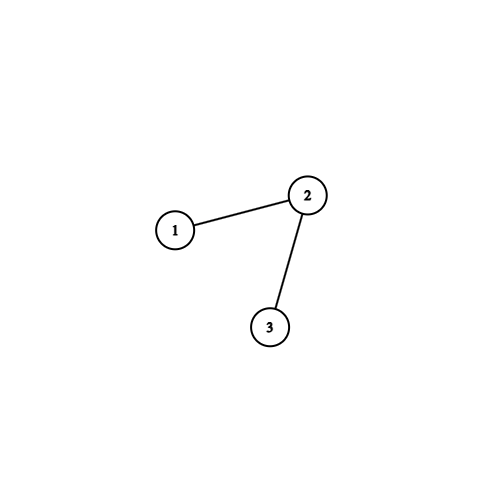
\includegraphics[keepaspectratio]{_main_files/fig/fig18.png}} & \(
\begin{array}{c|ccc}
\text{Vertices:} & 1 & 2 & 3 \\ \hline
1 & 0 & 1 & 1 \\
2 & 1 & 0 & 1 \\
3 & 1 & 1 & 0
\end{array}
\) \\
\end{longtable}
}

\subsection{\texorpdfstring{The Adjacency Matrix (\(A\))}{The Adjacency Matrix (A)}}\label{the-adjacency-matrix-a}

For a graph \(G = (V, E)\) with \(n\) labeled vertices \(\{1, 2, \dots, n\}\), the \textbf{adjacency matrix} \(A\) is an \(n \times n\) matrix where:

\[A(i, j) = \begin{cases} 1 & \text{if } (i, j) \in E \\ 0 & \text{if } (i, j) \notin E \end{cases}\]

\subsubsection{Matrix Properties}\label{matrix-properties}

\begin{itemize}
\item
  \textbf{Undirected Graphs}: \(A\) is symmetric (\(A(i, j) = A(j, i)\)). The sum of entries in row \(i\) equals the degree \(d(v_i)\).
\item
  \textbf{Simple Graphs}: The diagonal entries \(A(i, i) = 0\) because simple graphs have no self-loops.
\item
  \textbf{Paths of Length \(k\)}: The entry \(A^k(i, j)\) in the \(k\)-th matrix power gives the exact number of distinct walks of length \(k\) between vertex \(i\) and vertex \(j\).
\end{itemize}

\begin{center}\rule{0.5\linewidth}{0.5pt}\end{center}

\subsection{\texorpdfstring{The Incidence Matrix (\(T\))}{The Incidence Matrix (T)}}\label{the-incidence-matrix-t}

For a graph with \(n\) vertices and \(m\) edges, the \textbf{incidence matrix} \(T\) is an \(n \times m\) matrix mapping vertices (rows) directly to edges (columns).

\subsubsection{Undirected Graphs}\label{undirected-graphs}

\[T(i, k) = \begin{cases} 1 & \text{if vertex } i \text{ is incident with edge } k \\ 0 & \text{otherwise} \end{cases}\]

\subsubsection{Directed Graphs (Digraphs)}\label{directed-graphs-digraphs-1}

\[T(i, k) = \begin{cases} -1 & \text{if directed edge } k \text{ leaves vertex } i \\ 1 & \text{if directed edge } k \text{ enters vertex } i \\ 0 & \text{if vertex } i \text{ is not incident with edge } k \end{cases}\]

\subsubsection{Example 2.3}\label{example-2.3}

Consider a directed graph with vertices \(\{v_1, v_2, v_3\}\) and edges \(e_1 = (v_1, v_2), e_2 = (v_2, v_3), e_3 = (v_1, v_3)\):

\[\text{Incidence Matrix } T = \begin{pmatrix}  e_1 & e_2 & e_3 \\ -1 & 0 & -1 \\  1 & -1 & 0 \\  0 & 1 & 1  \end{pmatrix}\]

\begin{center}\rule{0.5\linewidth}{0.5pt}\end{center}

\subsection{The Adjacency List}\label{the-adjacency-list}

An \textbf{adjacency list} maintains an array or list of size \(n\), where each entry \(i\) points to a list of all vertices adjacent to vertex \(i\).

{\def\LTcaptype{none} % do not increment counter
\begin{longtable}[]{@{}ll@{}}
\toprule\noalign{}
Vertex & Neighbors \\
\midrule\noalign{}
\endhead
\bottomrule\noalign{}
\endlastfoot
1 & -\(\rightarrow\) {[}2{]} \(\rightarrow\) {[}3{]} \\
2 & -\(\rightarrow\) {[}1{]} \(\rightarrow\) {[}3{]} \\
3 & -\(\rightarrow\) {[}1{]} \(\rightarrow\) {[}2{]} \\
\end{longtable}
}

\subsection{Representation Comparison}\label{representation-comparison}

{\def\LTcaptype{none} % do not increment counter
\begin{longtable}[]{@{}
  >{\raggedright\arraybackslash}p{(\linewidth - 6\tabcolsep) * \real{0.2500}}
  >{\raggedright\arraybackslash}p{(\linewidth - 6\tabcolsep) * \real{0.2500}}
  >{\raggedright\arraybackslash}p{(\linewidth - 6\tabcolsep) * \real{0.2500}}
  >{\raggedright\arraybackslash}p{(\linewidth - 6\tabcolsep) * \real{0.2500}}@{}}
\toprule\noalign{}
\begin{minipage}[b]{\linewidth}\raggedright
Representation
\end{minipage} & \begin{minipage}[b]{\linewidth}\raggedright
Memory Complexity
\end{minipage} & \begin{minipage}[b]{\linewidth}\raggedright
Edge Lookup \((u, v)\)
\end{minipage} & \begin{minipage}[b]{\linewidth}\raggedright
Ideal Use Case
\end{minipage} \\
\midrule\noalign{}
\endhead
\bottomrule\noalign{}
\endlastfoot
\textbf{Adjacency Matrix} & \(O(n^2)\) & \(O(1)\) constant time & \textbf{Dense Graphs} (where \(\vert{}E\vert{} \approx n^2\)) \\
\textbf{Incidence Matrix} & \(O(n \cdot m)\) & \(O(m)\) search time & \textbf{Theoretical Algorithms \& Flows} \\
\textbf{Adjacency List} & \(O(n + m)\) & \(O(d(u))\) list search time & \textbf{Sparse Graphs} (where \(\vert{}E\vert{} \ll n^2\)) \\
\end{longtable}
}

\begin{center}\rule{0.5\linewidth}{0.5pt}\end{center}

\section{Chapter 2 Exercises}\label{chapter-2-exercises}

\begin{exercise}
\protect\hypertarget{exr:unnamed-chunk-21}{}\label{exr:unnamed-chunk-21}\leavevmode

\begin{enumerate}
\def\labelenumi{\arabic{enumi}.}
\tightlist
\item
  \textbf{Graph Isomorphism}: Are \(K_{3,3}\) and a cycle \(C_6\) with extra cross-edges isomorphic? List two graph invariants you can use to justify your answer.
\item
  \textbf{Complement Construction}: Draw the complement of a path graph \(P_4\). Is \(P_4\) self-complementary?
\item
  \textbf{Eulerian vs Hamiltonian}: Construct a graph that contains an Eulerian circuit but does \textbf{not} contain a Hamiltonian cycle.
\item
  \textbf{Adjacency Matrix Powers}: Given the adjacency matrix \(A = \begin{pmatrix} 0 & 1 & 1 \\ 1 & 0 & 1 \\ 1 & 1 & 0 \end{pmatrix}\), compute \(A^2\) and interpret what the entry \(A^2(1, 1)\) represents.
\end{enumerate}

\end{exercise}

\chapter{Chapter 3: Connectivity \& Graph Exploration}\label{chapter-3-connectivity-graph-exploration}

\section{3.1 Graph Connectivity}\label{graph-connectivity}

Understanding how vertices are linked to one another is a fundamental concept in graph theory. Connectivity determines whether information, traffic, or signals can flow between different points in a network.

\subsection{Connectivity in Undirected Graphs}\label{connectivity-in-undirected-graphs}

In an undirected graph \(G = (V, E)\), two vertices \(u\) and \(v\) are connected if there exists a walk between them.

\begin{itemize}
\item
  \textbf{Reachability Relation (\(\sim\))}: We define a relation \(u \sim v\) if there exists a walk starting at vertex \(u\) and ending at vertex \(v\).
\item
  \textbf{Equivalence Classes}: The relation \(\sim\) is an equivalence relation because it satisfies three key properties:
\end{itemize}

\begin{enumerate}
\def\labelenumi{\arabic{enumi}.}
\item
  \textbf{Reflexive}: \(u \sim u\) (a trivial walk of length \(0\) exists from \(u\) to itself).
\item
  \textbf{Symmetric}: If \(u \sim v\), then \(v \sim u\) (since edges in undirected graphs can be traversed in either direction).
\item
  \textbf{Transitive}: If \(u \sim v\) and \(v \sim w\), then \(u \sim w\) (by concatenating the two walks).
\end{enumerate}

Because \(\sim\) is an equivalence relation, it partitions the set of vertices \(V\) into disjoint equivalence classes called \textbf{connected components}.

\pandocbounded{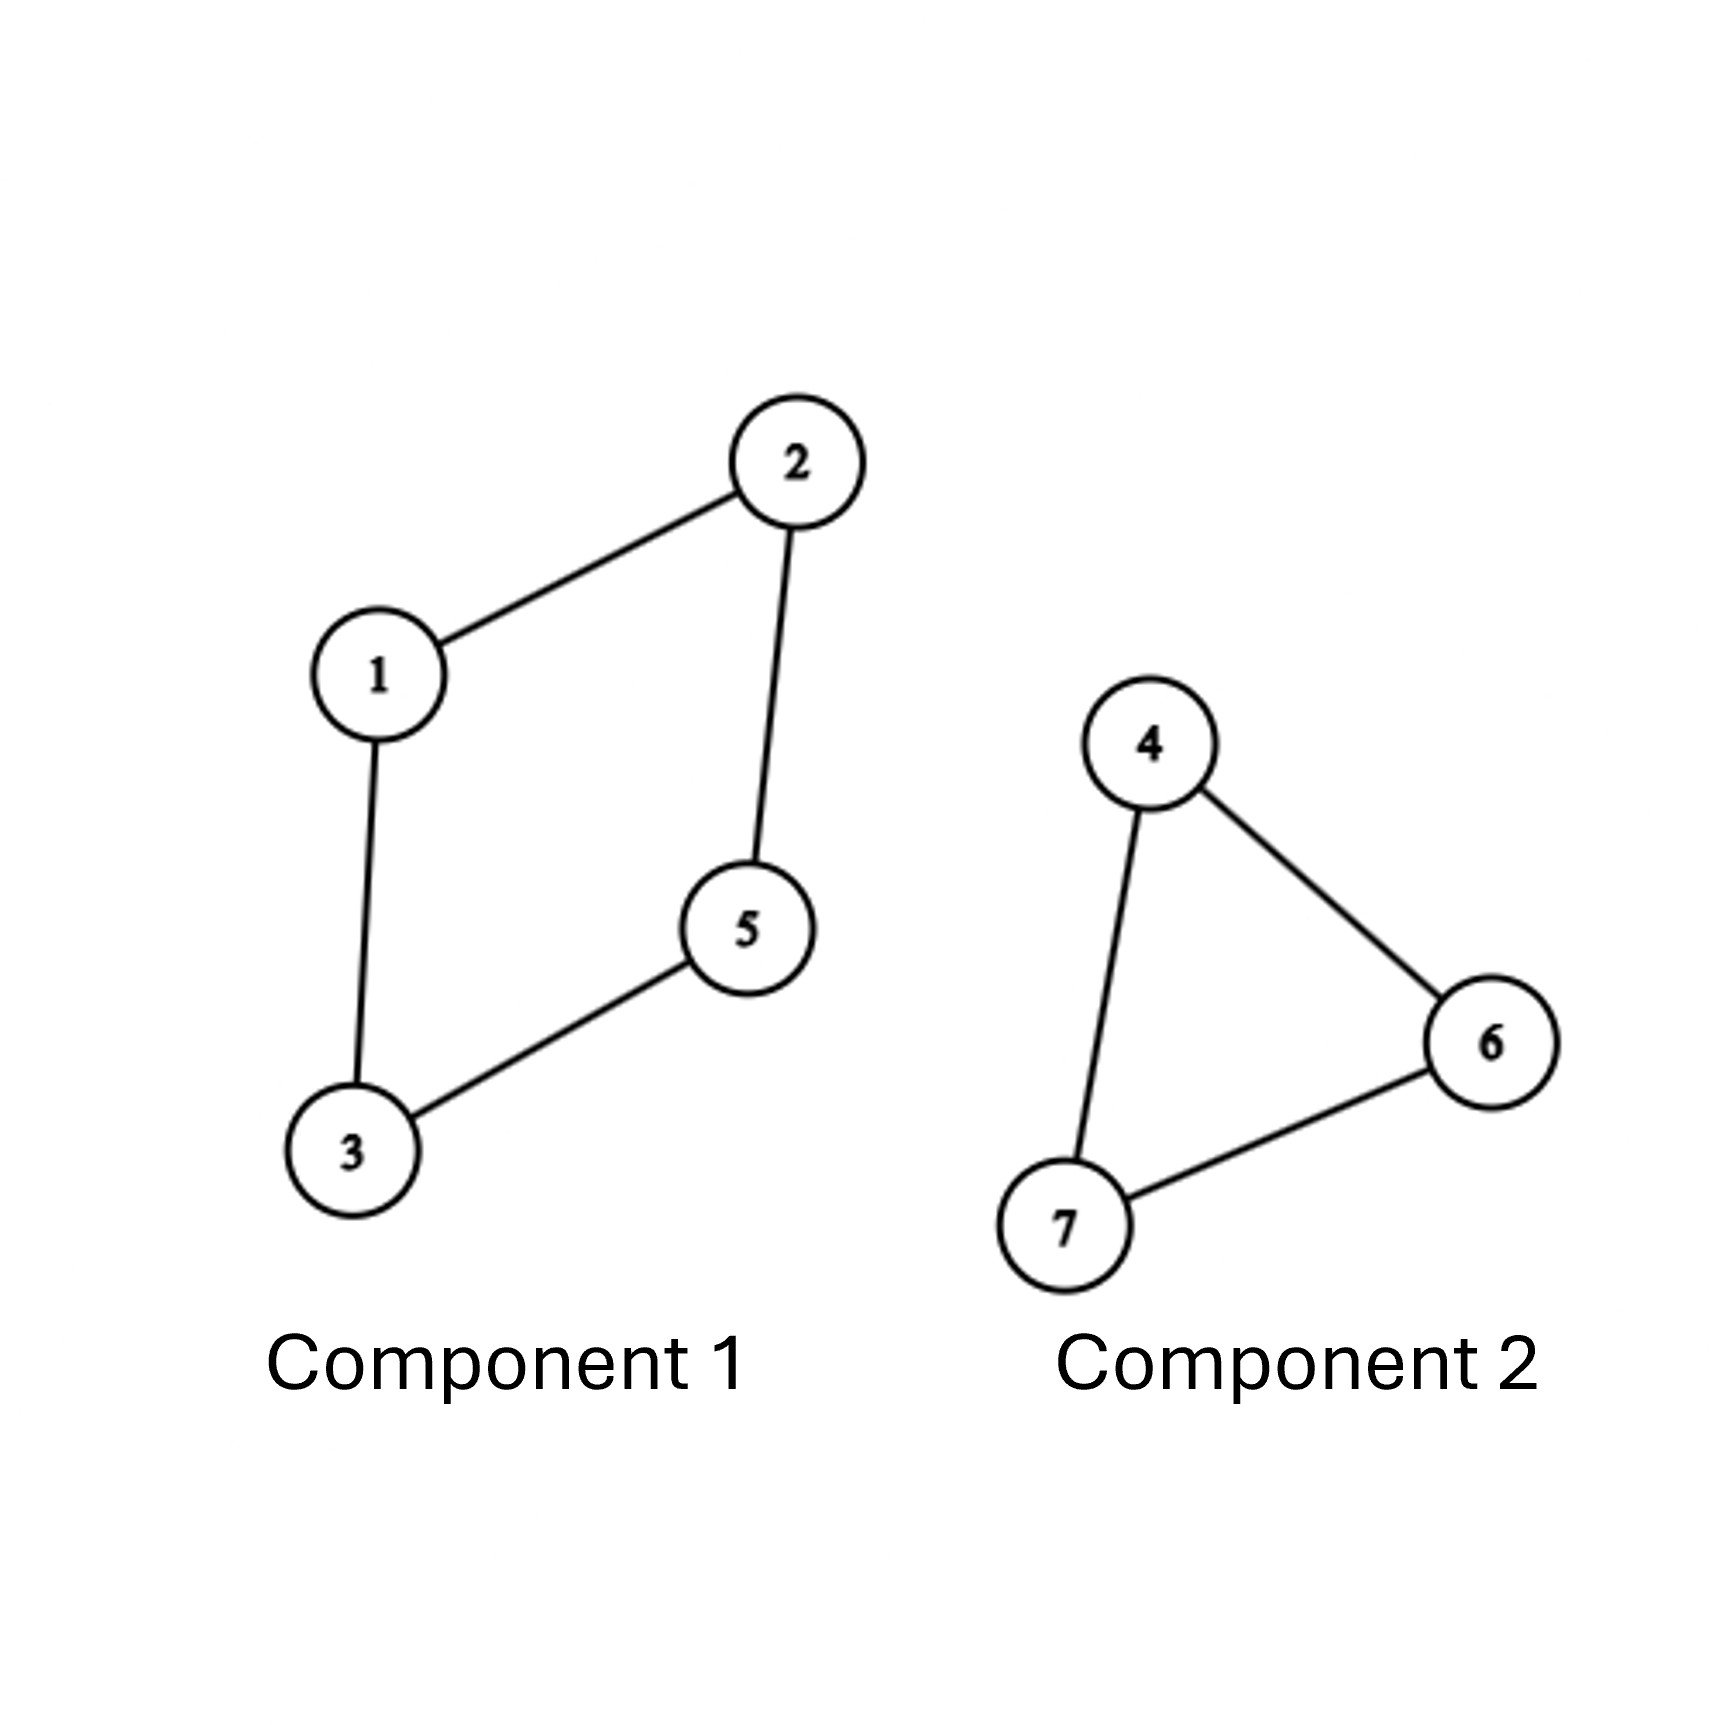
\includegraphics[keepaspectratio]{_main_files/fig/fig22.png}}

A graph is \textbf{connected} if it consists of exactly one connected component (meaning every vertex can reach every other vertex). Otherwise, it is \textbf{disconnected}.

\begin{center}\rule{0.5\linewidth}{0.5pt}\end{center}

\subsection{Strong Connectivity in Directed Graphs}\label{strong-connectivity-in-directed-graphs}

In directed graphs (digraphs), edge directions matter. The existence of a path from \(u\) to \(v\) does not guarantee a path from \(v\) to \(u\).

\begin{itemize}
\item
  \textbf{Strong Connectivity}: Two vertices \(u\) and \(v\) in a digraph are \textbf{strongly connected} if there exists a directed walk from \(u\) to \(v\) \textbf{and} a directed walk from \(v\) to \(u\).
\item
  \textbf{Strongly Connected Component (SCC)}: A maximal subgraph where every pair of vertices is mutually reachable.
\end{itemize}

\pandocbounded{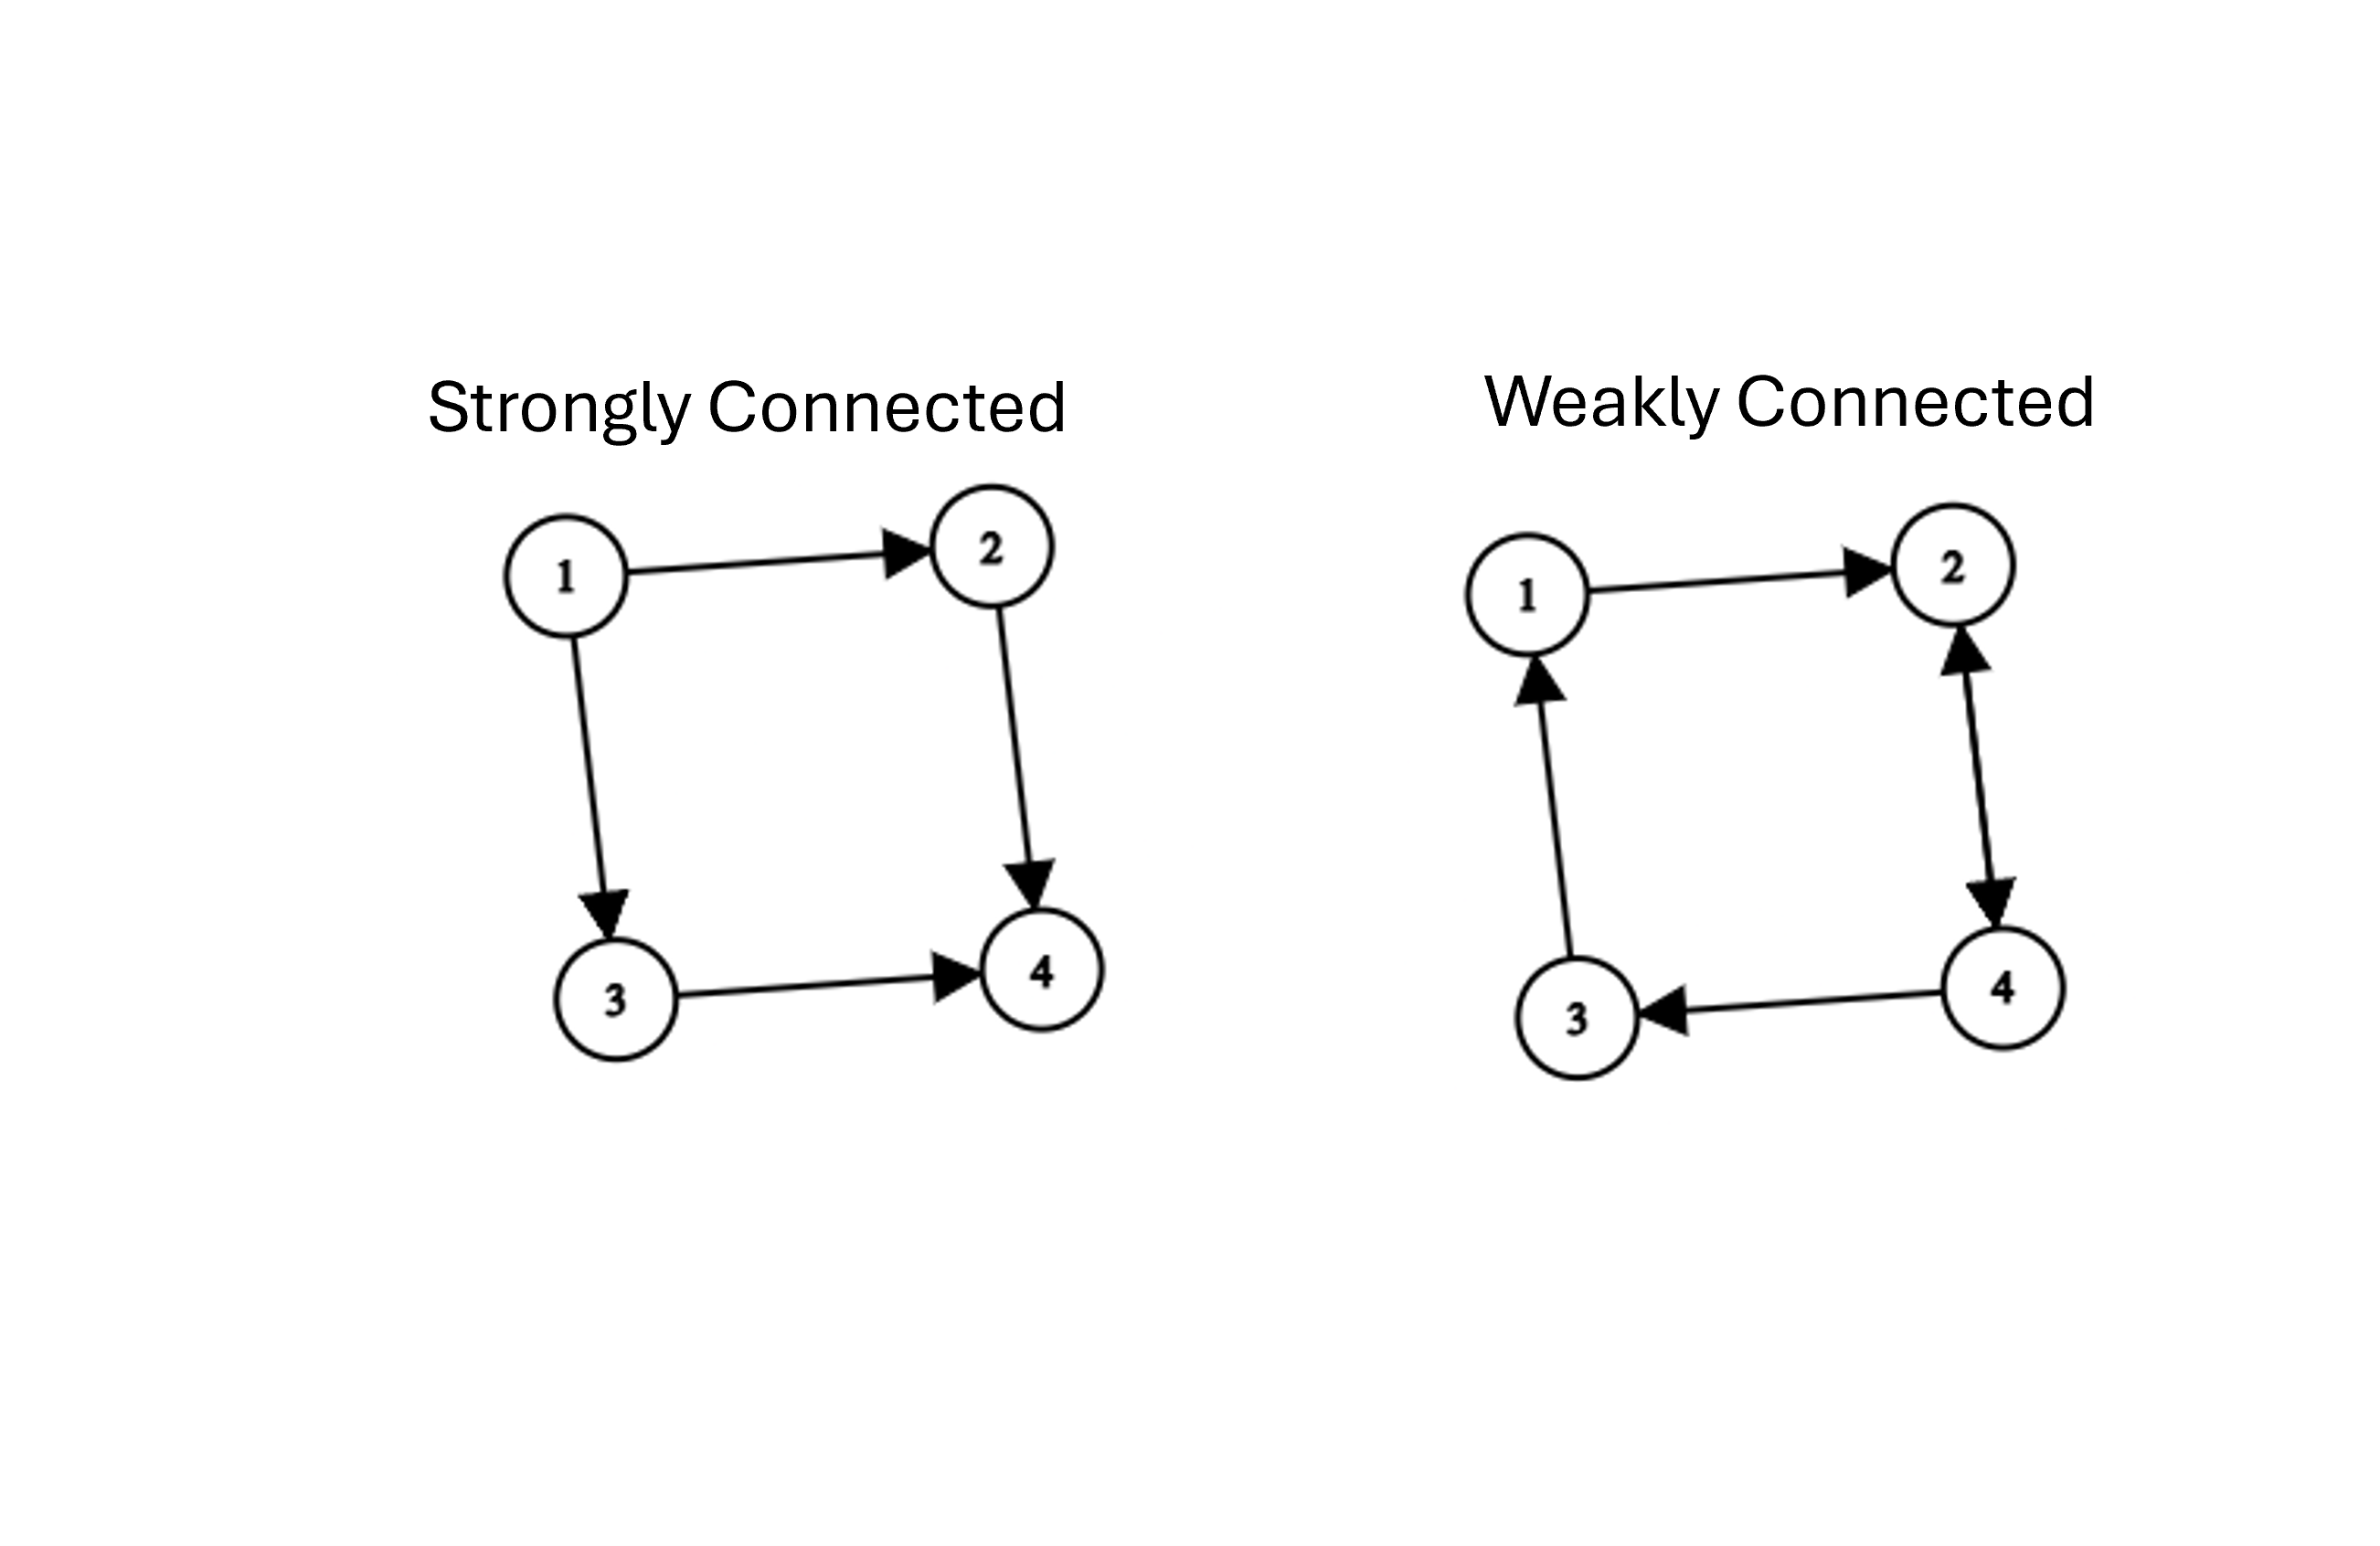
\includegraphics[keepaspectratio]{_main_files/fig/fig23.png}}

\subsubsection{Computing Strongly Connected Components}\label{computing-strongly-connected-components}

To formally define the SCC containing a vertex \(u\), denoted as \(C(u)\), we look at two reaching sets:

\begin{enumerate}
\def\labelenumi{\arabic{enumi}.}
\item
  \textbf{Forward Reachable Set (\(R_+(u)\))}: The set of all vertices \(v\) reachable from \(u\) via directed paths.
\item
  \textbf{Backward Reachable Set (\(R_-(u)\))}: The set of all vertices \(v\) that can reach \(u\) via directed paths.
\end{enumerate}

The strongly connected component of \(u\) is the intersection of these two sets:

\[C(u) = R_+(u) \cap R_-(u)\]

\begin{verbatim}
                 R+(u): Nodes u can reach
                          \
                           \  Intersection: C(u)
                            v /
                           ( u )
                            ^ \
                           /   \
                          /     v
                 R-(u): Nodes that can reach u
\end{verbatim}

\textbf{Algorithmic Insight}: Computing \(R_+(u)\) is straightforward---we run a standard search starting at \(u\). To compute \(R_-(u)\), we find all nodes that can reach \(u\) in \(G\), which is equivalent to finding all nodes reachable \textbf{from} \(u\) in the \textbf{transpose graph \(G^T\)} (where every directed edge is reversed). Matrix-wise, \(G^T\) corresponds to the transpose of the adjacency matrix, \(A^T\).

\begin{center}\rule{0.5\linewidth}{0.5pt}\end{center}

\section{Graph Exploration Algorithms}\label{graph-exploration-algorithms}

Graph exploration algorithms systematically visit the vertices and edges of a graph. They form the foundation for solving complex problems such as finding shortest paths, cycle detection, and identifying connected components.

\subsection{Generic Search Algorithm}\label{generic-search-algorithm}

The generic search algorithm maintains a set \(L\) of candidate vertices to explore.

\subsubsection{Generic Search Steps}\label{generic-search-steps}

\begin{enumerate}
\def\labelenumi{\arabic{enumi}.}
\item
  Initialize a set of discovered vertices \(L = \{s\}\), where \(s\) is the starting vertex. Mark \(s\) as visited.
\item
  While \(L\) is not empty:
\end{enumerate}

\begin{itemize}
\item
  Select an arbitrary vertex \(u \in L\).
\item
  Find an unvisited neighbor \(v\) adjacent to \(u\).
\item
  If such a \(v\) exists, mark \(v\) as visited and add \(v\) to \(L\).
\item
  If no unvisited neighbors exist for \(u\), remove \(u\) from \(L\).
\item
  \textbf{Complexity}: Takes \(O(V)\) main steps, but the specific execution order depends entirely on the data structure used to manage \(L\).
\end{itemize}

\begin{center}\rule{0.5\linewidth}{0.5pt}\end{center}

\subsection{Depth-First Search (DFS)}\label{depth-first-search-dfs}

Depth-First Search explores a graph by going as deep as possible along each branch before backtracking.

\begin{itemize}
\item
  \textbf{Data Structure}: Last-In, First-Out (\textbf{LIFO}) Stack (or recursion).
\item
  \textbf{Strategy}: Pick a start vertex, move to an unvisited neighbor, and immediately continue exploring from that new neighbor. When a vertex has no unvisited neighbors, backtrack to the previous vertex.
\end{itemize}

\begin{verbatim}
                     DFS Exploration Order
                              (1)
                             /   \
                           [1]   [4]
                           /       \
                         (2)       (4)
                        /
                      [2]
                      /
                    (3)
\end{verbatim}

\begin{figure}
\centering
\pandocbounded{\includegraphics[keepaspectratio,alt={Animated example of a depth-first search (Image Source: Wikipedia}]{_main_files/fig/fig24.gif}}
\caption{Animated example of a depth-first search (Image Source: Wikipedia}
\end{figure}

\subsubsection{DFS Algorithm Steps}\label{dfs-algorithm-steps}

\begin{enumerate}
\def\labelenumi{\arabic{enumi}.}
\tightlist
\item
  Push the starting vertex \(s\) onto the stack.
\item
  While the stack is not empty:
\end{enumerate}

\begin{itemize}
\item
  Pop the top vertex \(u\).
\item
  If \(u\) is not visited, mark it as visited.
\item
  Push all unvisited neighbors of \(u\) onto the stack.
\item
  \textbf{Time Complexity}: \(O(V + E)\) when using an adjacency list.
\item
  \textbf{Primary Applications}: Detecting cycles, topological sorting, finding strongly connected components, and pathfinding in mazes.
\end{itemize}

\begin{center}\rule{0.5\linewidth}{0.5pt}\end{center}

\subsection{Breadth-First Search (BFS)}\label{breadth-first-search-bfs}

Breadth-First Search explores the graph layer-by-layer, visiting all immediate neighbors of a vertex before moving deeper.

\begin{itemize}
\item
  \textbf{Data Structure}: First-In, First-Out (\textbf{FIFO}) Queue.
\item
  \textbf{Strategy}: Visit the starting node, then visit all of its direct neighbors (distance 1), then all neighbors of those neighbors (distance 2), and so on.
\end{itemize}

\begin{verbatim}
                     BFS Exploration Order
                              (1)  <-- Level 0
                             /   \
                           [1]   [1]
                           /       \
                         (2)-------(3) <-- Level 1
                          |
                         [2]
                          |
                         (4)           <-- Level 2
\end{verbatim}

\begin{figure}
\centering
\pandocbounded{\includegraphics[keepaspectratio,alt={Animated example of a BFS (Image Source: Wikipedia)}]{_main_files/fig/fig25.gif}}
\caption{Animated example of a BFS (Image Source: Wikipedia)}
\end{figure}

Black = explored, grey = queued to be explored later on

\subsubsection{BFS Algorithm Steps}\label{bfs-algorithm-steps}

\begin{enumerate}
\def\labelenumi{\arabic{enumi}.}
\tightlist
\item
  Enqueue the starting vertex \(s\) into the queue and mark it as visited.
\item
  While the queue is not empty:
\end{enumerate}

\begin{itemize}
\item
  Dequeue the front vertex \(u\).
\item
  For each unvisited neighbor \(v\) of \(u\):
\item
  Mark \(v\) as visited.
\item
  Enqueue \(v\).
\item
  \textbf{Time Complexity}: \(O(V + E)\) when using an adjacency list.
\item
  \textbf{Primary Applications}: Finding the shortest path in unweighted graphs, finding connected components, and computing graph diameter.
\end{itemize}

\begin{center}\rule{0.5\linewidth}{0.5pt}\end{center}

\section{Comparison of Exploration Algorithms}\label{comparison-of-exploration-algorithms}

{\def\LTcaptype{none} % do not increment counter
\begin{longtable}[]{@{}
  >{\raggedright\arraybackslash}p{(\linewidth - 8\tabcolsep) * \real{0.2000}}
  >{\raggedright\arraybackslash}p{(\linewidth - 8\tabcolsep) * \real{0.2000}}
  >{\raggedright\arraybackslash}p{(\linewidth - 8\tabcolsep) * \real{0.2000}}
  >{\raggedright\arraybackslash}p{(\linewidth - 8\tabcolsep) * \real{0.2000}}
  >{\raggedright\arraybackslash}p{(\linewidth - 8\tabcolsep) * \real{0.2000}}@{}}
\toprule\noalign{}
\begin{minipage}[b]{\linewidth}\raggedright
Algorithm
\end{minipage} & \begin{minipage}[b]{\linewidth}\raggedright
Data Structure
\end{minipage} & \begin{minipage}[b]{\linewidth}\raggedright
Traversal Strategy
\end{minipage} & \begin{minipage}[b]{\linewidth}\raggedright
Edge Types Discovered
\end{minipage} & \begin{minipage}[b]{\linewidth}\raggedright
Time Complexity
\end{minipage} \\
\midrule\noalign{}
\endhead
\bottomrule\noalign{}
\endlastfoot
\textbf{Generic Search} & Unordered Set \(L\) & Arbitrary selection & General reachability & \(O(V)\) main steps \\
\textbf{DFS} & LIFO Stack & Deep exploration via backtracking & Tree edges, Back edges, Forward edges, Cross edges & \(O(V + E)\) \\
\textbf{BFS} & FIFO Queue & Level-by-level exploration & Tree edges, Cross edges & \(O(V + E)\) \\
\end{longtable}
}

\begin{center}\rule{0.5\linewidth}{0.5pt}\end{center}

\section{Chapter 3 Exercises}\label{chapter-3-exercises}

\begin{enumerate}
\def\labelenumi{\arabic{enumi}.}
\item
  \textbf{Strongly Connected Components}: Given a directed graph \(G\), explain why taking the intersection \(R_+(u) \cap R_-(u)\) guarantees that all vertices in the resulting set belong to the same strongly connected component.
\item
  \textbf{Algorithm Execution}: Trace both BFS and DFS on a simple cycle graph \(C_5\) starting at vertex \(v_1\). List the order in which vertices are visited for each algorithm.
\item
  \textbf{Shortest Paths}: Prove that the tree generated by running Breadth-First Search (BFS) on an unweighted graph provides the shortest path (in terms of edge count) from the start vertex to all other reachable vertices.
\item
  \textbf{Graph Transpose}: Show that if \(A\) is the adjacency matrix of a digraph \(G\), then the transpose matrix \(A^T\) represents the graph \(G^T\) where all edge directions are reversed.
\end{enumerate}

\chapter{Planar Graphs}\label{planar-graphs}

\section{Planarity and Embeddings}\label{planarity-and-embeddings}

In real-world applications---such as designing printed circuit boards (PCBs), microchip layouts, and urban road networks---it is often necessary to draw or construct a graph without any edges crossing over one another.

\subsection{Definitions}\label{definitions-1}

\begin{definition}
\protect\hypertarget{def:unnamed-chunk-22}{}\label{def:unnamed-chunk-22}\leavevmode

\begin{itemize}
\item
  \textbf{Planar Graph}: A graph that can be drawn in a two-dimensional plane such that no two edges intersect except at a common vertex.
\item
  \textbf{Plane Graph (Plane Embedding)}: A specific drawing of a planar graph on a plane where no edges cross.
\end{itemize}

\end{definition}

\begin{verbatim}
  Non-Planar Representation of K4          Plane Embedding of K4
              (1)---(2)                            (1)---(2)
               | \ / |                              | \ / |
               |  X  |                              |  (4) |
               | / \ |                              | / \ |
              (3)---(4)                            (3)-----+
\end{verbatim}

\emph{(Note: \(K_4\) drawn with crossed diagonal edges is still a planar graph because it is isomorphic to a plane embedding where one vertex is pulled outside.)}

\subsection{Fáry's Theorem}\label{fuxe1rys-theorem}

A natural question arises: if a graph can be drawn without crossing edges using curved lines, can it also be drawn using only straight lines?

\begin{theorem}[Fáry's Theorem, 1948]
\protect\hypertarget{thm:unnamed-chunk-23}{}\label{thm:unnamed-chunk-23}Every simple planar graph can be embedded in the plane using straight-line segments for all of its edges.
\end{theorem}

\begin{center}\rule{0.5\linewidth}{0.5pt}\end{center}

\section{Euler's Formula and Regions}\label{eulers-formula-and-regions}

When a planar graph is drawn as a plane graph, its edges divide the plane into contiguous, enclosed areas called \textbf{regions} (or faces).

\begin{itemize}
\tightlist
\item
  \textbf{Boundary of a Region}: The set of edges enclosing that region.
\item
  \textbf{Unbounded (Outer) Region}: The single infinite region surrounding the entire drawing. Every plane graph has exactly one outer region.
\end{itemize}

\begin{figure}
\centering
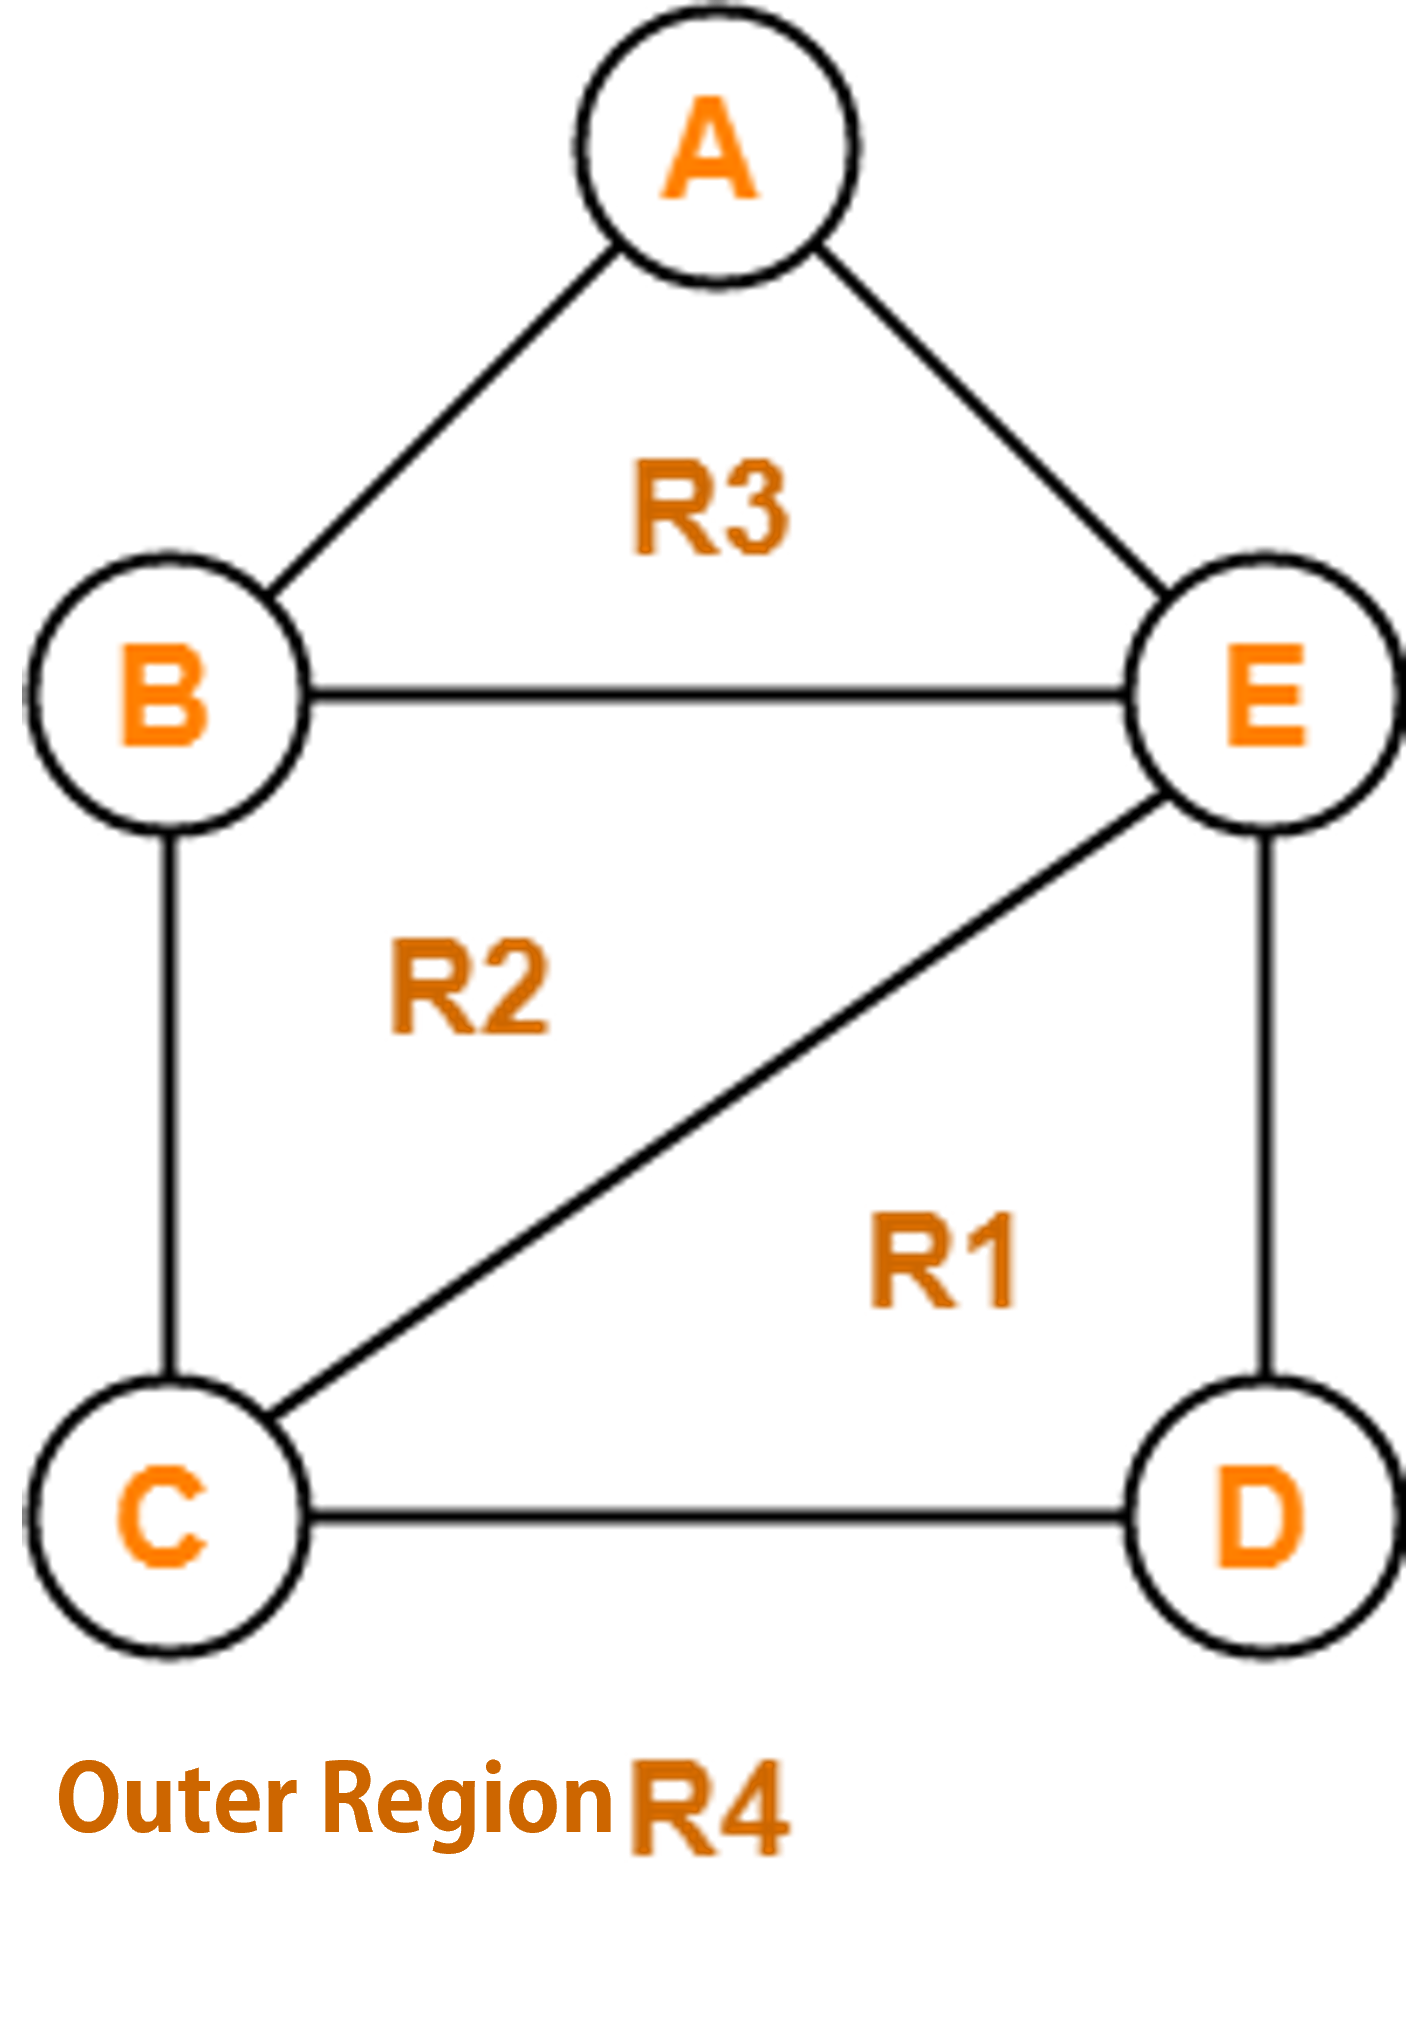
\includegraphics[width=0.3\linewidth,height=\textheight,keepaspectratio,alt={Image Credit: gatevidyalay.com}]{_main_files/fig/fig26.png}
\caption{Image Credit: gatevidyalay.com}
\end{figure}

In the plane graph above, there are 5 vertices (\(v=5\)), 6 edges (\(e=6\)), and 3 bounded regions plus 1 unbounded outer region, giving 4 total regions (\(r=4\)).

\begin{center}\rule{0.5\linewidth}{0.5pt}\end{center}

\subsection{Euler's Formula}\label{eulers-formula}

The fundamental relationship connecting the number of vertices, edges, and regions of a planar graph was discovered by Leonhard Euler.

\begin{theorem}[Euler's Formula]
\protect\hypertarget{thm:unnamed-chunk-24}{}\label{thm:unnamed-chunk-24}For any connected plane graph with \(v\) vertices, \(e\) edges, and \(r\) regions:

\[v - e + r = 2\]
\end{theorem}

\subsubsection{Generalized Euler's Formula}\label{generalized-eulers-formula}

If a planar graph is disconnected and consists of \(c\) connected components, the formula generalizes to:

\[v - e + r = c + 1\]

\subsubsection{Proof of Euler's Formula (By Induction on Edges)}\label{proof-of-eulers-formula-by-induction-on-edges}

\textbf{Base Case}:

Consider a connected graph with no cycles (a tree). A tree on \(v\) vertices has \(e = v - 1\) edges and creates no enclosed areas, leaving only \(1\) outer region (\(r = 1\)).

\[v - (v - 1) + 1 = 2\]

The formula holds for the base case.

\textbf{Inductive Step}:

Assume \(v - e + r = 2\) holds for all connected plane graphs with \(k\) edges. Let \(G\) be a connected plane graph with \(k + 1\) edges.

\begin{enumerate}
\def\labelenumi{\arabic{enumi}.}
\tightlist
\item
  Since \(G\) is not a tree, it must contain at least one cycle.
\item
  Select an edge \(e^*\) that belongs to a cycle. Removing \(e^*\) breaks the cycle, merging two adjacent regions into one.
\item
  The new graph \(G' = G \setminus \{e^*\}\) has \(v'=v\) vertices, \(e'=e-1\) edges, and \(r'=r-1\) regions.
\item
  By the induction hypothesis, \(v' - e' + r' = 2\).
\item
  Substituting the values: \(v - (e - 1) + (r - 1) = 2 \implies v - e + r = 2\).
\end{enumerate}

By mathematical induction, Euler's formula holds for all connected plane graphs.

\begin{center}\rule{0.5\linewidth}{0.5pt}\end{center}

\section{Invariants and Non-Planarity Bounds}\label{invariants-and-non-planarity-bounds}

Euler's formula allows us to derive strict upper bounds on how many edges a simple graph can have while remaining planar.

\subsection{Edge Bounds for Simple Planar Graphs}\label{edge-bounds-for-simple-planar-graphs}

\begin{theorem}[General Edge Bound]
\protect\hypertarget{thm:unnamed-chunk-25}{}\label{thm:unnamed-chunk-25}In any simple connected planar graph with \(v \ge 3\) vertices and \(e\) edges:

\[e \le 3v - 6\]
\end{theorem}

\begin{proof}
\leavevmode

\begin{enumerate}
\def\labelenumi{\arabic{enumi}.}
\tightlist
\item
  Every region in a simple planar graph must be bounded by at least 3 edges (since a simple graph has no self-loops or double edges, the smallest cycle length is 3).
\item
  Summing the degree of all regions gives \(\sum \text{deg}(r_i) \ge 3r\).
\item
  Since every edge bounds at most 2 regions, \(\sum \text{deg}(r_i) = 2e\). Thus, \(2e \ge 3r \implies r \le \frac{2}{3}e\).
\item
  Substitute \(r \le \frac{2}{3}e\) into Euler's formula (\(v - e + r = 2\)):
\end{enumerate}

\[v - e + \frac{2}{3}e \ge 2 \implies v - \frac{1}{3}e \ge 2 \implies e \le 3v - 6\]

\end{proof}

\begin{center}\rule{0.5\linewidth}{0.5pt}\end{center}

\begin{theorem}[Girth Bound]
\protect\hypertarget{thm:unnamed-chunk-27}{}\label{thm:unnamed-chunk-27}If a simple planar graph has a \textbf{girth} (length of its shortest cycle) of at least 4 (i.e., it contains no triangles), then:

\[e \le 2v - 4\]
\end{theorem}

\begin{proof}
Since the graph has no triangles, every region is bounded by at least 4 edges. Therefore, \(2e \ge 4r \implies r \le \frac{1}{2}e\).
Substituting this into Euler's formula gives \(v - e + \frac{1}{2}e \ge 2 \implies e \le 2v - 4\).
\end{proof}

\begin{center}\rule{0.5\linewidth}{0.5pt}\end{center}

\subsection{Degree Bounds}\label{degree-bounds}

\begin{theorem}
\protect\hypertarget{thm:unnamed-chunk-29}{}\label{thm:unnamed-chunk-29}Every simple planar graph contains at least one vertex with degree \(d(v) \le 5\).
\end{theorem}

\begin{proof}
Suppose every vertex in a simple planar graph \(G\) has degree \(d(v) \ge 6\).
By the Handshaking Lemma:

\[2e = \sum d(v) \ge 6v \implies e \ge 3v\]

However, Theorem 1 states that \(e \le 3v - 6\), creating a direct contradiction (\(3v \le e \le 3v - 6\)). Therefore, \(G\) must contain at least one vertex with \(d(v) \le 5\).
\end{proof}

\begin{center}\rule{0.5\linewidth}{0.5pt}\end{center}

\section{Characterizing Non-Planar Graphs}\label{characterizing-non-planar-graphs}

Not all graphs are planar. The two canonical non-planar graphs are:

\begin{enumerate}
\def\labelenumi{\arabic{enumi}.}
\item
  \textbf{\(K_5\)}: The complete graph on 5 vertices.
\item
  \textbf{\(K_{3,3}\)}: The complete bipartite graph on 3+3 vertices (often called the \emph{utility graph}).
\end{enumerate}

\begin{verbatim}
         K5 (Complete Graph)              K3,3 (Utility Graph)
               (1)                            (u1)   (u2)   (u3)
              / | \                            | \   / | \   / |
            (2) | (3)                          |  \ /  |  \ /  |
            | \ | / |                          |   X   |   X   |
            (4)-(5)-+                          |  / \  |  / \  |
                                              (v1)   (v2)   (v3)
\end{verbatim}

\begin{figure}
\centering
\pandocbounded{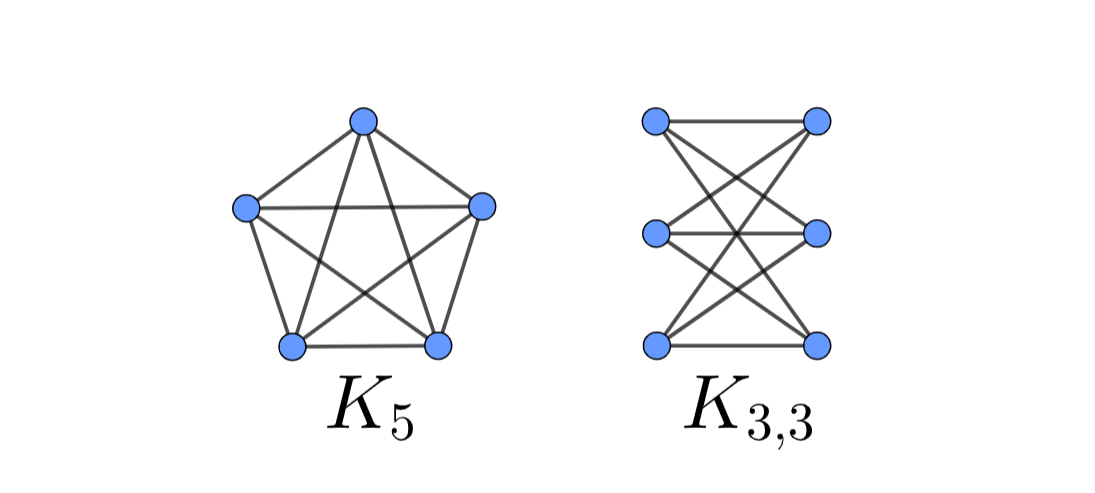
\includegraphics[keepaspectratio,alt={Image credit:https://medium.com/math-simplified/graph-theory-101-why-all-non-planar-graphs-contain-k\%E2\%82\%81-or-k\%E2\%82\%83-\%E2\%82\%83-c3ad48d6798e}]{_main_files/fig/fig27.png}}
\caption{Image credit:\url{https://medium.com/math-simplified/graph-theory-101-why-all-non-planar-graphs-contain-k\%E2\%82\%81-or-k\%E2\%82\%83-\%E2\%82\%83-c3ad48d6798e}}
\end{figure}

\subsection{Proving Non-Planarity}\label{proving-non-planarity}

\begin{example}[$K_5$ is Non-Planar]
\protect\hypertarget{exm:unnamed-chunk-31}{}\label{exm:unnamed-chunk-31}For \(K_5\), \(v = 5\) and \(e = \binom{5}{2} = 10\).
Using Theorem 1 (\(e \le 3v - 6\)):

\[10 \le 3(5) - 6 = 9 \quad \text{(False)}\]

Since \(10 \le 9\) is false, \(K_5\) cannot be planar.
\end{example}

\begin{example}[$K_{3,3}$ is Non-Planar]
\protect\hypertarget{exm:unnamed-chunk-32}{}\label{exm:unnamed-chunk-32}For \(K_{3,3}\), \(v = 6\) and \(e = 3 \times 3 = 9\).
Since \(K_{3,3}\) is bipartite, it contains no odd cycles (girth \(\ge 4\)). Using Theorem 2 (\(e \le 2v - 4\)):

\[9 \le 2(6) - 4 = 8 \quad \text{(False)}\]

Since \(9 \le 8\) is false, \(K_{3,3}\) cannot be planar.
\end{example}

\begin{center}\rule{0.5\linewidth}{0.5pt}\end{center}

\subsection{Kuratowski's Theorem}\label{kuratowskis-theorem}

How can we determine if an arbitrary complex graph is planar?

\begin{itemize}
\tightlist
\item
  \textbf{Edge Subdivision}: Inserting a vertex of degree 2 into an edge, splitting it into two adjacent edges.
\item
  \textbf{Subdivision of a Graph}: A graph obtained by performing a sequence of edge subdivisions on \(G\).
\end{itemize}

\begin{verbatim}
     Original Edge               Subdivided Edge
        (u)---(v)                 (u)---(w)---(v)
\end{verbatim}

\begin{theorem}[Kuratowski's Theorem(1930)]
\protect\hypertarget{thm:unnamed-chunk-33}{}\label{thm:unnamed-chunk-33}A finite graph is planar \textbf{if and only if} it does not contain a subgraph that is a subdivision of \(K_5\) or \(K_{3,3}\).
\end{theorem}

\begin{center}\rule{0.5\linewidth}{0.5pt}\end{center}

\section{Chapter 4 Summary Table}\label{chapter-4-summary-table}

{\def\LTcaptype{none} % do not increment counter
\begin{longtable}[]{@{}
  >{\raggedright\arraybackslash}p{(\linewidth - 4\tabcolsep) * \real{0.3333}}
  >{\raggedright\arraybackslash}p{(\linewidth - 4\tabcolsep) * \real{0.3333}}
  >{\raggedright\arraybackslash}p{(\linewidth - 4\tabcolsep) * \real{0.3333}}@{}}
\toprule\noalign{}
\begin{minipage}[b]{\linewidth}\raggedright
Property / Bound
\end{minipage} & \begin{minipage}[b]{\linewidth}\raggedright
Formula / Condition
\end{minipage} & \begin{minipage}[b]{\linewidth}\raggedright
Context / Application
\end{minipage} \\
\midrule\noalign{}
\endhead
\bottomrule\noalign{}
\endlastfoot
\textbf{Euler's Formula} & \(v - e + r = 2\) & Connected plane graphs \\
\textbf{General Edge Bound} & \(e \le 3v - 6\) & Simple planar graphs (\(v \ge 3\)) \\
\textbf{Triangle-Free Edge Bound} & \(e \le 2v - 4\) & Planar graphs with girth \(\ge 4\) \\
\textbf{Minimum Degree Invariant} & \(\min d(v) \le 5\) & All simple planar graphs \\
\textbf{Non-Planarity Criterion} & Subdivisions of \(K_5\) or \(K_{3,3}\) & Kuratowski's Theorem \\
\end{longtable}
}

\begin{center}\rule{0.5\linewidth}{0.5pt}\end{center}

\section{Chapter 4 Exercises}\label{chapter-4-exercises}

\begin{enumerate}
\def\labelenumi{\arabic{enumi}.}
\tightlist
\item
  \textbf{Euler's Formula Application}: A connected plane graph has 12 vertices, and every vertex has degree 3. How many edges and regions does the graph have?
\item
  \textbf{Polyhedron Proof}: Prove that no convex polyhedron can be constructed such that every face is bounded by 6 or more edges.
\item
  \textbf{Planarity Verification}: A simple planar graph \(G\) has 10 vertices and is bipartite. What is the maximum number of edges \(G\) can have?
\item
  \textbf{Kuratowski Subdivision}: Draw \(K_5\) and subdivide one of its edges by adding a new vertex. Is the resulting graph planar? Explain using Kuratowski's Theorem.
\end{enumerate}

\chapter{Trees \& Spanning Trees}\label{trees-spanning-trees}

\section{Basic Properties of Trees}\label{basic-properties-of-trees}

Trees are among the most fundamental and heavily utilized graph structures in mathematics and computer science. They represent minimally connected networks and form the backbone of hierarchical structures, search algorithms, and data structures.

\subsection{Definitions}\label{definitions-2}

\begin{itemize}
\tightlist
\item
  \textbf{Tree}: A connected, undirected simple graph that contains no cycles (an acyclic connected graph).
\item
  \textbf{Forest}: An acyclic graph whose connected components are trees.
\item
  \textbf{Leaf (Terminal Vertex)}: A vertex of degree 1 in a tree.
\item
  \textbf{Internal Vertex}: A vertex of degree greater than 1.
\end{itemize}

\begin{verbatim}
       Tree (1 Component)                     Forest (2 Components)
              (1)                               (1)           (5)
             /   \                             /   \         /   \
           (2)   (3)                         (2)   (3)     (6)   (7)
          /   \                             /   \
        (4)   (5)                         (4)   (5)
\end{verbatim}

\begin{center}\rule{0.5\linewidth}{0.5pt}\end{center}

\subsection{Equivalent Characterizations of Trees}\label{equivalent-characterizations-of-trees}

For any simple graph \(T = (V, E)\) with \(n\) vertices, the following statements are logically equivalent:

\begin{enumerate}
\def\labelenumi{\arabic{enumi}.}
\tightlist
\item
  \(T\) is a tree (connected and acyclic).
\item
  \(T\) is connected and has exactly \(n - 1\) edges.
\item
  \(T\) is acyclic and has exactly \(n - 1\) edges.
\item
  There exists a \textbf{unique simple path} between every pair of vertices in \(T\).
\item
  \(T\) is minimally connected: removing any edge disconnects \(T\) (every edge is a bridge).
\item
  \(T\) is maximally acyclic: adding any edge between non-adjacent vertices creates exactly one cycle.
\end{enumerate}

\subsubsection{\texorpdfstring{Proof Sketch: Every Tree Has \(n - 1\) Edges}{Proof Sketch: Every Tree Has n - 1 Edges}}\label{proof-sketch-every-tree-has-n---1-edges}

\textbf{Proof (By Induction on \(n\)):}

\begin{itemize}
\tightlist
\item
  \textbf{Base Case (\(n=1\)):} A tree with \(1\) vertex has \(0\) edges (\(1 - 1 = 0\)). The base case holds.
\item
  \textbf{Inductive Step:} Assume every tree with \(k\) vertices has \(k - 1\) edges. Let \(T\) be a tree with \(k + 1\) vertices (\(k \ge 1\)).
\end{itemize}

\begin{enumerate}
\def\labelenumi{\arabic{enumi}.}
\tightlist
\item
  Since \(T\) is connected and acyclic, \(T\) must contain at least one leaf vertex \(v\) with \(d(v) = 1\).
\item
  Remove \(v\) and its single incident edge \(e\). The resulting graph \(T' = T \setminus \{v\}\) remains connected and acyclic, so \(T'\) is a tree on \(k\) vertices.
\item
  By the inductive hypothesis, \(T'\) has \(k - 1\) edges.
\item
  Adding \(v\) and \(e\) back gives \(T\) a total of \((k - 1) + 1 = k\) edges.
\end{enumerate}

By induction, every tree with \(n\) vertices contains \(n - 1\) edges.

\begin{center}\rule{0.5\linewidth}{0.5pt}\end{center}

\section{5.2 Spanning Trees}\label{spanning-trees}

When analyzing a connected graph, we often seek a minimal connected backbone that preserves reachability while eliminating redundant cycles.

\subsection{Definition}\label{definition}

Given a connected graph \(G = (V, E)\), a \textbf{spanning tree} \(T = (V, E')\) is a subgraph that is a tree and contains \textbf{all} vertices of \(G\) (\(V(T) = V(G)\)).

\begin{verbatim}
       Original Graph G                      Spanning Tree T
           (1)---(2)                            (1)---(2)
            | \ / |                              |     |
            |  X  |                              |     |
            | / \ |                              |     |
           (3)---(4)                            (3)   (4)
\end{verbatim}

\subsubsection{Key Properties}\label{key-properties}

\begin{itemize}
\tightlist
\item
  A graph \(G\) has a spanning tree \textbf{if and only if} \(G\) is connected.
\item
  If \(G\) has \(n\) vertices and \(m\) edges, any spanning tree \(T\) selects exactly \(n - 1\) edges.
\item
  The \(m - (n - 1)\) edges present in \(G\) but omitted from \(T\) are called \textbf{cotree edges} (or chords).
\end{itemize}

\begin{center}\rule{0.5\linewidth}{0.5pt}\end{center}

\subsection{Counting Spanning Trees}\label{counting-spanning-trees}

\subsubsection{1. Cayley's Formula (Labeled Trees)}\label{cayleys-formula-labeled-trees}

How many distinct labeled spanning trees can be constructed on \(n\) vertices?

\textbf{Theorem (Cayley's Formula, 1889):}

The number of distinct labeled trees on \(n\) vertices (or the number of spanning trees of the complete graph \(K_n\)) is:

\[\tau(K_n) = n^{n-2}\]

\begin{itemize}
\tightlist
\item
  \textbf{Example 5.1:}
\item
  For \(n = 3\): \(\tau(K_3) = 3^{3-2} = 3\) spanning trees.
\item
  For \(n = 4\): \(\tau(K_4) = 4^{4-2} = 16\) spanning trees.
\end{itemize}

\begin{center}\rule{0.5\linewidth}{0.5pt}\end{center}

\subsubsection{2. The Matrix-Tree Theorem (Kirchhoff's Theorem)}\label{the-matrix-tree-theorem-kirchhoffs-theorem}

To compute the exact number of spanning trees \(\tau(G)\) for an \textbf{arbitrary} simple graph \(G\), we use its Laplacian Matrix.

\textbf{Definition (Laplacian Matrix \(L\)):}

Given a graph with \(n\) vertices, its Laplacian matrix \(L\) is defined as:

\[L = D - A\]

where \(D\) is the diagonal degree matrix (\(D_{ii} = d(v_i)\)) and \(A\) is the adjacency matrix.

\[L_{i,j} = \begin{cases} d(v_i) & \text{if } i = j \\ -1 & \text{if } i \neq j \text{ and } (v_i, v_j) \in E \\ 0 & \text{otherwise} \end{cases}\]

\textbf{Theorem (Kirchhoff's Matrix-Tree Theorem):}

For any connected graph \(G\), the number of spanning trees \(\tau(G)\) equals the absolute value of \textbf{any cofactor} of its Laplacian matrix \(L\).

\[\tau(G) = \det(L_{i,j})\]

\emph{(where \(L_{i,j}\) is the submatrix formed by deleting row \(i\) and column \(j\) from \(L\))}.

\begin{center}\rule{0.5\linewidth}{0.5pt}\end{center}

\section{5.3 Fundamental Cycles and Cutsets}\label{fundamental-cycles-and-cutsets}

Spanning trees provide a structured coordinate system for analyzing cycles and cuts in a graph.

\subsection{Fundamental Cycles}\label{fundamental-cycles}

Let \(T\) be a spanning tree of a connected graph \(G = (V, E)\).

\begin{itemize}
\tightlist
\item
  Adding any non-tree edge \(e \in E \setminus E(T)\) to \(T\) creates \textbf{exactly one cycle}.
\item
  This cycle is called the \textbf{fundamental cycle} associated with edge \(e\).
\item
  Since there are \(m - (n - 1)\) non-tree edges, \(T\) defines a basis of \(m - n + 1\) fundamental cycles.
\end{itemize}

\begin{verbatim}
  Spanning Tree T (Solid) + Non-Tree Edge e (Dashed) -> Fundamental Cycle
                     (1)-----------(2)
                      |             |
                      |  e (dashed) |
                      |  . . . . .  |
                      | .          .|
                     (3)-----------(4)
\end{verbatim}

\begin{center}\rule{0.5\linewidth}{0.5pt}\end{center}

\subsection{Fundamental Cutsets}\label{fundamental-cutsets}

Removing any tree edge \(e \in E(T)\) splits \(T\) into two disconnected components with vertex sets \(V_1\) and \(V_2\).

\begin{itemize}
\tightlist
\item
  The set of all edges in \(G\) that connect a vertex in \(V_1\) to a vertex in \(V_2\) forms a \textbf{fundamental cutset} (or fundamental edge cut) associated with \(e\).
\item
  Each fundamental cutset contains \textbf{exactly one} edge from the spanning tree \(T\).
\end{itemize}

\begin{center}\rule{0.5\linewidth}{0.5pt}\end{center}

\section{5.4 Minimum Spanning Trees (MST)}\label{minimum-spanning-trees-mst}

In weighted networks---such as fiber-optic cabling, electrical grids, or transportation routes---each edge \(e\) has an associated cost or weight \(w(e)\).

\subsection{The Minimum Spanning Tree Problem}\label{the-minimum-spanning-tree-problem}

Given a connected, weighted graph \(G = (V, E, w)\), find a spanning tree \(T\) that minimizes the total edge weight:

\[w(T) = \sum_{e \in E(T)} w(e)\]

\begin{center}\rule{0.5\linewidth}{0.5pt}\end{center}

\subsection{Key Theoretical Properties of MSTs}\label{key-theoretical-properties-of-msts}

\begin{enumerate}
\def\labelenumi{\arabic{enumi}.}
\tightlist
\item
  \textbf{Cut Property:}
  For any cut \((S, V \setminus S)\) of \(G\), the lightest edge \(e\) crossing the cut must belong to \textbf{every} Minimum Spanning Tree of \(G\).
\item
  \textbf{Cycle Property:}
  For any cycle \(C\) in \(G\), the heaviest edge \(e\) in \(C\) cannot belong to \textbf{any} Minimum Spanning Tree (assuming edge weights are distinct).
\item
  \textbf{Uniqueness:}
  If all edge weights in \(G\) are distinct, \(G\) has a \textbf{unique} Minimum Spanning Tree.
\end{enumerate}

\begin{center}\rule{0.5\linewidth}{0.5pt}\end{center}

\subsection{Greedy MST Algorithms}\label{greedy-mst-algorithms}

\subsubsection{1. Kruskal's Algorithm (Edge-Centric)}\label{kruskals-algorithm-edge-centric}

Kruskal's algorithm builds the MST by adding edges in increasing order of weight, avoiding cycles at every step.

\begin{verbatim}
                     Kruskal's Algorithm Step
  1. Sort all edges by weight.
  2. Pick the smallest edge. If it forms a cycle with the 
     current forest, discard it; otherwise, add it.
  3. Repeat until n - 1 edges are selected.
\end{verbatim}

\begin{itemize}
\tightlist
\item
  \textbf{Data Structure:} Disjoint-Set Union (DSU / Find-Union).
\item
  \textbf{Time Complexity:} \(O(E \log E)\) or \(O(E \log V)\) due to edge sorting.
\end{itemize}

\begin{center}\rule{0.5\linewidth}{0.5pt}\end{center}

\subsubsection{2. Prim's Algorithm (Vertex-Centric)}\label{prims-algorithm-vertex-centric}

Prim's algorithm grows a single tree component outwards from an arbitrary starting vertex.

\begin{verbatim}
                      Prim's Algorithm Step
  1. Start with a single vertex in tree set S.
  2. Find the minimum-weight edge (u, v) such that u in S and v not in S.
  3. Add v to S and include (u, v) in the tree.
  4. Repeat until S contains all vertices.
\end{verbatim}

\begin{itemize}
\tightlist
\item
  \textbf{Data Structure:} Priority Queue / Binary Heap.
\item
  \textbf{Time Complexity:} \(O(E \log V)\) with a binary heap, or \(O(E + V \log V)\) using a Fibonacci heap.
\end{itemize}

\begin{center}\rule{0.5\linewidth}{0.5pt}\end{center}

\section{Chapter 5 Comparison Table}\label{chapter-5-comparison-table}

{\def\LTcaptype{none} % do not increment counter
\begin{longtable}[]{@{}
  >{\raggedright\arraybackslash}p{(\linewidth - 4\tabcolsep) * \real{0.3333}}
  >{\raggedright\arraybackslash}p{(\linewidth - 4\tabcolsep) * \real{0.3333}}
  >{\raggedright\arraybackslash}p{(\linewidth - 4\tabcolsep) * \real{0.3333}}@{}}
\toprule\noalign{}
\begin{minipage}[b]{\linewidth}\raggedright
Algorithm / Theorem
\end{minipage} & \begin{minipage}[b]{\linewidth}\raggedright
Strategy / Core Idea
\end{minipage} & \begin{minipage}[b]{\linewidth}\raggedright
Primary Output / Complexity
\end{minipage} \\
\midrule\noalign{}
\endhead
\bottomrule\noalign{}
\endlastfoot
\textbf{Cayley's Formula} & Combinatorial enumeration (\(n^{n-2}\)) & Number of labeled trees on \(n\) vertices \\
\textbf{Kirchhoff's Theorem} & Determinant of Laplacian submatrix (\(\det L_{i,j}\)) & Exact count of spanning trees for any graph \(G\) \\
\textbf{Kruskal's Algorithm} & Global edge sorting + Disjoint Sets & Minimum Spanning Tree in \(O(E \log V)\) time \\
\textbf{Prim's Algorithm} & Local tree expansion + Priority Queue & Minimum Spanning Tree in \(O(E \log V)\) time \\
\end{longtable}
}

\begin{center}\rule{0.5\linewidth}{0.5pt}\end{center}

\section{Chapter 5 Exercises}\label{chapter-5-exercises}

\begin{enumerate}
\def\labelenumi{\arabic{enumi}.}
\tightlist
\item
  \textbf{Tree Bounds}: Prove that every tree with \(n \ge 2\) vertices has at least 2 leaves.
\item
  \textbf{Cayley's Formula Application}: How many distinct spanning trees can be formed from the complete graph \(K_5\)?
\item
  \textbf{Laplacian Matrix Computation}: Construct the Laplacian matrix \(L\) for a cycle graph \(C_4\) and use Kirchhoff's Matrix-Tree Theorem to compute its total number of spanning trees.
\item
  \textbf{MST Execution}: Given a graph \(G\) with vertices \(\{A, B, C, D\}\) and weighted edges \((A,B)=2, (B,C)=3, (A,C)=1, (C,D)=4, (B,D)=5\), trace both Kruskal's and Prim's algorithms step-by-step to construct the MST.
\end{enumerate}

\chapter{Chapter 6: Graph Colorings \& Chromatic Numbers}\label{chapter-6-graph-colorings-chromatic-numbers}

\section{6.1 Vertex Coloring and Chromatic Number}\label{vertex-coloring-and-chromatic-number}

Graph coloring is one of the most widely studied areas of graph theory, with applications ranging from scheduling algorithms and register allocation in compilers to radio frequency assignment.

\subsection{Definitions}\label{definitions-3}

\begin{itemize}
\tightlist
\item
  \textbf{Proper Vertex \(k\)-Coloring}: An assignment of \(k\) colors to the vertices of a graph \(G = (V, E)\) such that no two adjacent vertices share the same color.
\end{itemize}

\[f: V \to \{1, 2, \dots, k\} \quad \text{such that } (u, v) \in E \implies f(u) \neq f(v)\]

\begin{itemize}
\tightlist
\item
  \textbf{\(k\)-Colorable}: A graph \(G\) is \(k\)-colorable if it admits a proper vertex \(k\)-coloring.
\item
  \textbf{Chromatic Number \(\chi(G)\)}: The minimum number of colors required to properly color the vertices of \(G\).
\end{itemize}

\begin{verbatim}
       Proper 3-Coloring of C5                    Color Classes
               (Red)                              Color 1 (Red):   {1}
              /     \                             Color 2 (Blue):  {2, 4}
        (Blue)       (Green)                      Color 3 (Green): {3, 5}
         |               |
       (Green)-------(Blue)
\end{verbatim}

\subsection{Independent Sets and Color Classes}\label{independent-sets-and-color-classes}

In a proper vertex coloring, all vertices assigned the same color form an \textbf{independent set} (a set of vertices with no pairwise adjacent edges).

\begin{itemize}
\tightlist
\item
  A proper \(k\)-coloring partitions the vertex set \(V\) into \(k\) disjoint independent sets called \textbf{color classes} \(V_1, V_2, \dots, V_k\).
\item
  \textbf{Independence Number \(\alpha(G)\)}: The size of the largest independent set in \(G\).
\end{itemize}

Because each color class \(V_i\) can contain at most \(\alpha(G)\) vertices, we obtain the fundamental lower bound:

\[\chi(G) \ge \frac{\vert{}V\vert{}}{\alpha(G)}\]

\begin{center}\rule{0.5\linewidth}{0.5pt}\end{center}

\section{6.2 Chromatic Numbers for Standard Graph Families}\label{chromatic-numbers-for-standard-graph-families}

The chromatic number varies significantly depending on the structural symmetry and density of the graph.

{\def\LTcaptype{none} % do not increment counter
\begin{longtable}[]{@{}
  >{\raggedright\arraybackslash}p{(\linewidth - 6\tabcolsep) * \real{0.2500}}
  >{\raggedright\arraybackslash}p{(\linewidth - 6\tabcolsep) * \real{0.2500}}
  >{\raggedright\arraybackslash}p{(\linewidth - 6\tabcolsep) * \real{0.2500}}
  >{\raggedright\arraybackslash}p{(\linewidth - 6\tabcolsep) * \real{0.2500}}@{}}
\toprule\noalign{}
\begin{minipage}[b]{\linewidth}\raggedright
Graph Family
\end{minipage} & \begin{minipage}[b]{\linewidth}\raggedright
Notation
\end{minipage} & \begin{minipage}[b]{\linewidth}\raggedright
Chromatic Number \(\chi(G)\)
\end{minipage} & \begin{minipage}[b]{\linewidth}\raggedright
Description / Condition
\end{minipage} \\
\midrule\noalign{}
\endhead
\bottomrule\noalign{}
\endlastfoot
\textbf{Empty Graph} & \(E_n\) & \(1\) & No edges; all vertices can share 1 color. \\
\textbf{Complete Graph} & \(K_n\) & \(n\) & Every vertex is adjacent to every other vertex. \\
\textbf{Bipartite Graph} & \(K_{m,n}\) & \(2\) & Vertices can be partitioned into 2 independent sets. \\
\textbf{Tree / Forest} & \(T\) & \(2\) & Every tree with \(n \ge 2\) is 2-colorable (bipartite). \\
\textbf{Cycle Graph} & \(C_n\) & \(\begin{cases} 2 & \text{if } n \text{ is even} \\ 3 & \text{if } n \text{ is odd} \end{cases}\) & Odd cycles require 3 colors due to parity loop closure. \\
\textbf{Wheel Graph} & \(W_n\) & \(\begin{cases} 3 & \text{if } n \text{ is even} \\ 4 & \text{if } n \text{ is odd} \end{cases}\) & Central hub vertex connects to an outer cycle \(C_{n-1}\). \\
\end{longtable}
}

\begin{center}\rule{0.5\linewidth}{0.5pt}\end{center}

\section{6.3 Bounds on Chromatic Numbers}\label{bounds-on-chromatic-numbers}

Determining the exact chromatic number \(\chi(G)\) for arbitrary graphs is an NP-hard problem. Consequently, we rely on structural invariants to establish upper and lower bounds.

\subsection{Lower Bounds}\label{lower-bounds}

\begin{enumerate}
\def\labelenumi{\arabic{enumi}.}
\tightlist
\item
  \textbf{Clique Number Bounds:}
\end{enumerate}

\begin{itemize}
\tightlist
\item
  \textbf{Clique (\(K_r\))}: A complete subgraph where every pair of vertices is adjacent.
\item
  \textbf{Clique Number \(\omega(G)\)}: The size of the largest clique in \(G\).
\item
  Since every vertex in a clique of size \(\omega(G)\) requires a distinct color:
\end{itemize}

\[\chi(G) \ge \omega(G)\]

\begin{enumerate}
\def\labelenumi{\arabic{enumi}.}
\setcounter{enumi}{1}
\tightlist
\item
  \textbf{Independence Number Bounds:}
\end{enumerate}

\[\chi(G) \ge \frac{\vert{}V\vert{}}{\alpha(G)}\]

\begin{center}\rule{0.5\linewidth}{0.5pt}\end{center}

\subsection{Upper Bounds}\label{upper-bounds}

\begin{enumerate}
\def\labelenumi{\arabic{enumi}.}
\tightlist
\item
  \textbf{Maximum Degree Bound:}
  If a graph \(G\) has maximum vertex degree \(\Delta(G)\), a simple greedy coloring algorithm guarantees that:
\end{enumerate}

\[\chi(G) \le \Delta(G) + 1\]

\begin{enumerate}
\def\labelenumi{\arabic{enumi}.}
\setcounter{enumi}{1}
\tightlist
\item
  \textbf{Brooks' Theorem (1941):}
  Can we improve upon the naive \(\Delta(G) + 1\) bound? For almost all connected graphs, yes.
  \textbf{Theorem (Brooks' Theorem):}
  For any connected, simple graph \(G\),
\end{enumerate}

\[\chi(G) \le \Delta(G)\]

\textbf{unless} \(G\) is a \textbf{complete graph} (\(K_n\)) or an \textbf{odd cycle} (\(C_2k+1\)), in which case \(\chi(G) = \Delta(G) + 1\).

\begin{center}\rule{0.5\linewidth}{0.5pt}\end{center}

\section{6.4 Planar Graph Coloring and Map Theorems}\label{planar-graph-coloring-and-map-theorems}

Map coloring was the historical driving force behind the development of graph coloring theory.

\begin{verbatim}
                  Dual Graph Transformation
        Map Regions                        Dual Graph
      +-------------+                      (R1)-------(R2)
      |   R1 | R2   |                       |    \   /  |
      +------+------+   =======>            |     (R3)  |
      |     R3      |                       |    /   \  |
      +-------------+                      (R4)-------(R5)
\end{verbatim}

\subsection{The Dual Graph}\label{the-dual-graph}

Any political map can be converted into a planar graph by placing a vertex inside each region (country/province) and drawing an edge between two vertices if their corresponding regions share a common border.

\subsection{Planar Coloring Theorems}\label{planar-coloring-theorems}

\begin{enumerate}
\def\labelenumi{\arabic{enumi}.}
\tightlist
\item
  \textbf{Six Color Theorem:}
  Every simple planar graph is 6-colorable (\(\chi(G) \le 6\)).
  \emph{Proof Sketch:} Uses the planar invariant that every planar graph contains a vertex \(v\) with \(d(v) \le 5\), followed by induction on \(\vert{}V\vert{}\).
\item
  \textbf{Five Color Theorem (Heawood, 1890):}
  Every simple planar graph is 5-colorable (\(\chi(G) \le 5\)).
\item
  \textbf{The Four Color Theorem (Appel \& Haken, 1976):}
  \textbf{Theorem:} Every simple planar graph is 4-colorable.
\end{enumerate}

\[\text{If } G \text{ is planar} \implies \chi(G) \le 4\]

\emph{(Note: The Four Color Theorem was the first major mathematical theorem to be proved using a computer, verifying 1,936 reducible configuration cases.)}

\begin{center}\rule{0.5\linewidth}{0.5pt}\end{center}

\section{6.5 Edge Coloring \& Chromatic Index}\label{edge-coloring-chromatic-index}

Instead of coloring vertices, edge coloring assigns colors to edges such that no two adjacent edges (edges sharing a common vertex) have the same color.

\subsection{Definitions}\label{definitions-4}

\begin{itemize}
\tightlist
\item
  \textbf{Proper Edge \(k\)-Coloring}: A mapping \(c: E \to \{1, 2, \dots, k\}\) such that \(e_1 \cap e_2 \neq \emptyset \implies c(e_1) \neq c(e_2)\).
\item
  \textbf{Chromatic Index \(\chi'(G)\)}: The minimum number of colors needed to properly color the edges of \(G\).
\end{itemize}

\begin{verbatim}
         Proper Edge Coloring of K3               Vizing's Bound
                   (1)                            Delta(G) = 2
                  /   \                           Chi'(G)  = 3
           Red   /     \  Blue                    Class 1: Chi'(G) = Delta(G)
                /       \                         Class 2: Chi'(G) = Delta(G) + 1
              (2)-------(3)
                 Green
\end{verbatim}

\subsection{Fundamental Bounds on Edge Coloring}\label{fundamental-bounds-on-edge-coloring}

\begin{enumerate}
\def\labelenumi{\arabic{enumi}.}
\tightlist
\item
  \textbf{Trivial Lower Bound:}
  Since a vertex with degree \(\Delta(G)\) has \(\Delta(G)\) incident edges that must all receive different colors:
\end{enumerate}

\[\chi'(G) \ge \Delta(G)\]

\begin{enumerate}
\def\labelenumi{\arabic{enumi}.}
\setcounter{enumi}{1}
\tightlist
\item
  \textbf{Vizing's Theorem (1964):}
  \textbf{Theorem:} For any simple graph \(G\), the chromatic index \(\chi'(G)\) satisfies:
\end{enumerate}

\[\Delta(G) \le \chi'(G) \le \Delta(G) + 1\]

This remarkable result partitions all simple graphs into two distinct categories:
* \textbf{Class 1 Graphs}: \(\chi'(G) = \Delta(G)\) (e.g., all bipartite graphs).
* \textbf{Class 2 Graphs}: \(\chi'(G) = \Delta(G) + 1\) (e.g., odd cycles \(C_{2k+1}\)).

\begin{center}\rule{0.5\linewidth}{0.5pt}\end{center}

\section{Chapter 6 Comparison Table}\label{chapter-6-comparison-table}

{\def\LTcaptype{none} % do not increment counter
\begin{longtable}[]{@{}
  >{\raggedright\arraybackslash}p{(\linewidth - 6\tabcolsep) * \real{0.2500}}
  >{\raggedright\arraybackslash}p{(\linewidth - 6\tabcolsep) * \real{0.2500}}
  >{\raggedright\arraybackslash}p{(\linewidth - 6\tabcolsep) * \real{0.2500}}
  >{\raggedright\arraybackslash}p{(\linewidth - 6\tabcolsep) * \real{0.2500}}@{}}
\toprule\noalign{}
\begin{minipage}[b]{\linewidth}\raggedright
Metric / Theorem
\end{minipage} & \begin{minipage}[b]{\linewidth}\raggedright
Target Element
\end{minipage} & \begin{minipage}[b]{\linewidth}\raggedright
Bound / Formula
\end{minipage} & \begin{minipage}[b]{\linewidth}\raggedright
Key Conditions / Exceptions
\end{minipage} \\
\midrule\noalign{}
\endhead
\bottomrule\noalign{}
\endlastfoot
\textbf{Clique Bound} & Vertices & \(\chi(G) \ge \omega(G)\) & Lower bound based on complete subgraphs \\
\textbf{Brooks' Theorem} & Vertices & \(\chi(G) \le \Delta(G)\) & Excludes \(K_n\) and odd cycles \(C_{2k+1}\) \\
\textbf{Four Color Theorem} & Vertices & \(\chi(G) \le 4\) & Applies strictly to planar graphs \\
\textbf{Vizing's Theorem} & Edges & \(\chi'(G) \in \{\Delta(G), \Delta(G) + 1\}\) & Holds for all simple graphs \\
\end{longtable}
}

\begin{center}\rule{0.5\linewidth}{0.5pt}\end{center}

\section{Chapter 6 Exercises}\label{chapter-6-exercises}

\begin{enumerate}
\def\labelenumi{\arabic{enumi}.}
\tightlist
\item
  \textbf{Chromatic Number Calculation}: Determine the chromatic number \(\chi(G)\) and independence number \(\alpha(G)\) for the Grötzsch graph (or an odd cycle \(C_7\)).
\item
  \textbf{Brooks' Theorem Verification}: Identify whether the complete bipartite graph \(K_{3,3}\) satisfies \(\chi(G) \le \Delta(G)\).
\item
  \textbf{Planar Map Coloring}: Construct a planar graph with 6 vertices that has \(\chi(G) = 4\).
\item
  \textbf{Vizing's Classification}: Classify the cycle graphs \(C_5\) and \(C_6\) into Class 1 or Class 2 according to Vizing's Theorem.
\end{enumerate}

\chapter{Chapter 7: Network Flows \& Matching}\label{chapter-7-network-flows-matching}

\section{7.1 Flow Networks and Capacities}\label{flow-networks-and-capacities}

Network flows extend graph theory into directed, weighted systems where quantities---such as data packets, fluid, traffic, or commodities---travel from a source to a destination through capacity-constrained channels.

\subsection{Definitions}\label{definitions-5}

\begin{itemize}
\tightlist
\item
  \textbf{Flow Network}: A directed graph \(G = (V, E)\) with two special vertices: a \textbf{source} \(s \in V\) (where flow originates) and a \textbf{sink} \(t \in V\) (where flow terminates).
\item
  \textbf{Capacity Function \(c(u, v)\)}: A non-negative real mapping \(c: E \to \mathbb{R}_{\ge 0}\) representing the maximum allowable flow along edge \((u, v)\).
\item
  \textbf{Flow Function \(f(u, v)\)}: A real-valued mapping \(f: E \to \mathbb{R}_{\ge 0}\) satisfying three core conditions:
\end{itemize}

\begin{verbatim}
                  Capacity Constraint: f(u, v) <= c(u, v)
                           Flow: 3 / Cap: 5
                      (u)----------------->(v)
\end{verbatim}

\subsection{Core Conditions for Valid Flows}\label{core-conditions-for-valid-flows}

\begin{enumerate}
\def\labelenumi{\arabic{enumi}.}
\tightlist
\item
  \textbf{Capacity Constraint}: For every edge \((u, v) \in E\):
\end{enumerate}

\[0 \le f(u, v) \le c(u, v)\]

\begin{enumerate}
\def\labelenumi{\arabic{enumi}.}
\setcounter{enumi}{1}
\tightlist
\item
  \textbf{Skew Symmetry}: \(f(u, v) = -f(v, u)\).
\item
  \textbf{Flow Conservation}: For every vertex \(u \in V \setminus \{s, t\}\), the total incoming flow equals the total outgoing flow:
\end{enumerate}

\[\sum_{w \in V} f(w, u) = \sum_{v \in V} f(u, v)\]

\subsection{Value of a Flow}\label{value-of-a-flow}

The \textbf{value} of a flow \(\vert{}f\vert{}\) is the net flow leaving the source \(s\) (which, by conservation, equals the net flow entering the sink \(t\)):

\[\vert{}f\vert{} = \sum_{v \in V} f(s, v)\]

\begin{center}\rule{0.5\linewidth}{0.5pt}\end{center}

\section{7.2 Cuts and the Max-Flow Min-Cut Theorem}\label{cuts-and-the-max-flow-min-cut-theorem}

To determine the absolute upper bound on flow through a network, we examine cuts that physically separate the source from the sink.

\subsection{Definitions}\label{definitions-6}

\begin{itemize}
\tightlist
\item
  \textbf{\(s\)-\(t\) Cut}: A partition of the vertex set \(V\) into two disjoint sets \(S\) and \(T\) such that \(s \in S\) and \(t \in T\).
\item
  \textbf{Capacity of a Cut \(c(S, T)\)}: The sum of capacities of all edges directed from \(S\) to \(T\):
\end{itemize}

\[c(S, T) = \sum_{u \in S, v \in T, (u,v) \in E} c(u, v)\]

\emph{(Note: Edges directed from \(T\) back to \(S\) do NOT contribute to the capacity of the cut.)}

\begin{verbatim}
                       s-t Cut Partitioning
         [ S Set (Source) ]          [ T Set (Sink) ]
              (s)------(u)            (v)------(t)
                        |              ^
                        +------------->|  Edge (u, v) crosses cut
                           c(u, v)
\end{verbatim}

\begin{center}\rule{0.5\linewidth}{0.5pt}\end{center}

\subsection{The Max-Flow Min-Cut Theorem}\label{the-max-flow-min-cut-theorem}

The relationship between maximum flow values and minimum cut capacities forms the central foundation of network flow theory.

\textbf{Theorem (Ford \& Fulkerson, 1956):}

In any flow network \(G\), the maximum value of an \(s\)-\(t\) flow is equal to the minimum capacity of an \(s\)-\(t\) cut:

\[\max \vert{}f\vert{} = \min c(S, T)\]

\subsubsection{Key Corollaries}\label{key-corollaries}

\begin{itemize}
\tightlist
\item
  For any valid flow \(f\) and any valid \(s\)-\(t\) cut \((S, T)\), \(\vert{}f\vert{} \le c(S, T)\).
\item
  A flow \(f\) is maximum \textbf{if and only if} its residual network contains no augmenting path.
\end{itemize}

\begin{center}\rule{0.5\linewidth}{0.5pt}\end{center}

\section{7.3 Algorithms for Computing Maximum Flow}\label{algorithms-for-computing-maximum-flow}

\subsection{1. The Ford-Fulkerson Method}\label{the-ford-fulkerson-method}

The Ford-Fulkerson method greedily increases flow by finding \textbf{augmenting paths} in a \textbf{residual network} \(G_f\).

\begin{itemize}
\tightlist
\item
  \textbf{Residual Capacity \(c_f(u, v)\)}:
\end{itemize}

\[c_f(u, v) = c(u, v) - f(u, v)\]

\begin{itemize}
\item
  Forward edge capacity: \(c(u, v) - f(u, v)\) (remaining capacity).
\item
  Backward edge capacity: \(f(u, v)\) (ability to push flow back and cancel it).
\item
  \textbf{Augmenting Path}: A directed path from \(s\) to \(t\) in the residual graph \(G_f\) where every edge has positive residual capacity \(c_f(u, v) > 0\).
\end{itemize}

\begin{verbatim}
                    Residual Graph Augmentation
      Original Flow               Residual Edges
     f=3 / c=5                   Forward: 2  (Remaining)
    (u)--------->(v)   ======>  (u)=========>
                                   <=========(v)
                                 Backward: 3 (Cancelable)
\end{verbatim}

\begin{itemize}
\tightlist
\item
  \textbf{Time Complexity}: \(O(E \cdot \vert{}f^*\vert{})\), where \(\vert{}f^*\vert{}\) is the maximum flow value. (If capacities are irrational, Ford-Fulkerson may fail to terminate or converge to the wrong value).
\end{itemize}

\begin{center}\rule{0.5\linewidth}{0.5pt}\end{center}

\subsection{2. The Edmonds-Karp Algorithm}\label{the-edmonds-karp-algorithm}

Edmonds and Karp specified that the augmenting path in the Ford-Fulkerson method should always be the \textbf{shortest path} (in terms of edge count) from \(s\) to \(t\) in \(G_f\).

\begin{itemize}
\tightlist
\item
  \textbf{Path Selection Strategy}: Breadth-First Search (BFS).
\item
  \textbf{Time Complexity}: \(O(V \cdot E^2)\), independent of edge capacity values.
\end{itemize}

\begin{center}\rule{0.5\linewidth}{0.5pt}\end{center}

\section{7.4 Matching in Bipartite Graphs}\label{matching-in-bipartite-graphs}

Network flows can directly solve matching problems in bipartite graphs, such as assigning workers to tasks, students to courses, or medical residents to hospitals.

\subsection{Definitions}\label{definitions-7}

\begin{itemize}
\tightlist
\item
  \textbf{Matching \(M\)}: A subset of edges \(M \subseteq E\) such that no two edges in \(M\) share a common vertex.
\item
  \textbf{Maximum Matching}: A matching containing the maximum possible number of edges.
\item
  \textbf{Perfect Matching}: A matching that covers every vertex in the graph (\(\vert{}M\vert{} = \vert{}V\vert{} / 2\)).
\end{itemize}

\begin{verbatim}
         Bipartite Matching                  Flow Network Transformation
          Set A      Set B                   (s) ---> Set A ---> Set B ---> (t)
           (a1)------(b1)                    All edge capacities = 1
           (a2)------(b2)                    Max Flow = Max Matching
           (a3)------(b3)
\end{verbatim}

\begin{center}\rule{0.5\linewidth}{0.5pt}\end{center}

\subsection{Converting Bipartite Matching to Network Flow}\label{converting-bipartite-matching-to-network-flow}

To find the maximum matching in a bipartite graph \(G = (A \cup B, E)\):

\begin{enumerate}
\def\labelenumi{\arabic{enumi}.}
\tightlist
\item
  Create a directed graph \(G' = (V', E')\).
\item
  Add a super source \(s\) and draw directed edges \((s, a)\) with capacity \(1\) for all \(a \in A\).
\item
  Direct all original edges from \(A\) to \(B\) with capacity \(1\).
\item
  Add a super sink \(t\) and draw directed edges \((b, t)\) with capacity \(1\) for all \(b \in B\).
\item
  Run Edmonds-Karp to compute maximum flow.
\end{enumerate}

\textbf{Theorem:}

The maximum flow value \(\vert{}f^*\vert{}\) in \(G'\) equals the maximum matching size \(\vert{}M^*\vert{}\) in \(G\).

\begin{center}\rule{0.5\linewidth}{0.5pt}\end{center}

\subsection{Hall's Marriage Theorem}\label{halls-marriage-theorem}

Hall's Theorem provides the exact condition for when a bipartite graph contains a matching that covers all vertices of one partition.

\textbf{Theorem (Hall's Condition, 1935):}

Let \(G = (A \cup B, E)\) be a bipartite graph. There exists a matching that covers every vertex in \(A\) \textbf{if and only if} for every subset \(S \subseteq A\), the size of its neighborhood \(N(S)\) satisfies:

\[\vert{}N(S)\vert{} \ge \vert{}S\vert{}\]

\begin{verbatim}
                   Hall's Condition Failure
             Subset S (|S|=2)         Neighborhood N(S) (|N(S)|=1)
                   (a1)----+
                           |-------> (b1)
                   (a2)----+
             Condition Violated: |N(S)| < |S|  (1 < 2)
\end{verbatim}

\begin{center}\rule{0.5\linewidth}{0.5pt}\end{center}

\section{Chapter 7 Comparison Table}\label{chapter-7-comparison-table}

{\def\LTcaptype{none} % do not increment counter
\begin{longtable}[]{@{}
  >{\raggedright\arraybackslash}p{(\linewidth - 6\tabcolsep) * \real{0.2500}}
  >{\raggedright\arraybackslash}p{(\linewidth - 6\tabcolsep) * \real{0.2500}}
  >{\raggedright\arraybackslash}p{(\linewidth - 6\tabcolsep) * \real{0.2500}}
  >{\raggedright\arraybackslash}p{(\linewidth - 6\tabcolsep) * \real{0.2500}}@{}}
\toprule\noalign{}
\begin{minipage}[b]{\linewidth}\raggedright
Concept / Algorithm
\end{minipage} & \begin{minipage}[b]{\linewidth}\raggedright
Primary Mechanism
\end{minipage} & \begin{minipage}[b]{\linewidth}\raggedright
Time Complexity / Formula
\end{minipage} & \begin{minipage}[b]{\linewidth}\raggedright
Key Application
\end{minipage} \\
\midrule\noalign{}
\endhead
\bottomrule\noalign{}
\endlastfoot
\textbf{Max-Flow Min-Cut} & Duality of flows and cuts & \(\max \Vert{}f\Vert{} = \min c(S, T)\) & System bottlenecks \& capacities \\
\textbf{Ford-Fulkerson} & Arbitrary residual augmentation & \(O(E \cdot \Vert{}f^*\Vert{})\) & Small integer flow networks \\
\textbf{Edmonds-Karp} & BFS shortest augmenting paths & \(O(V \cdot E^2)\) & General maximum flow problems \\
\textbf{Hall's Theorem} & Neighborhood size check & \(\Vert{}N(S)\Vert{} \ge \Vert{}S\Vert{}\) & Bipartite matching existence \\
\end{longtable}
}

\begin{center}\rule{0.5\linewidth}{0.5pt}\end{center}

\section{Chapter 7 Exercises}\label{chapter-7-exercises}

\begin{enumerate}
\def\labelenumi{\arabic{enumi}.}
\tightlist
\item
  \textbf{Max-Flow Calculation}: Given a flow network with source \(s\), sink \(t\), and capacities \((s,u)=4, (s,v)=2, (u,v)=1, (u,t)=3, (v,t)=5\), compute the maximum flow and identify the minimum \(s\)-\(t\) cut.
\item
  \textbf{Hall's Condition Application}: Check if a matching covering \(A\) exists for \(A = \{1, 2, 3\}, B = \{x, y, z\}\) with edges \((1,x), (1,y), (2,x), (3,x)\).
\item
  \textbf{Cut Capacity Computation}: If \(S = \{s, u\}\) and \(T = \{v, t\}\), calculate \(c(S, T)\) if edge capacities are \((s,v)=3, (u,v)=2, (u,t)=4, (v,u)=1\).
\item
  \textbf{Bipartite Reduction}: Prove that if every vertex in a \(k\)-regular bipartite graph has degree \(k \ge 1\), the graph contains a perfect matching.
\end{enumerate}

\chapter{Chapter 8: Spectral \& Algebraic Graph Theory}\label{chapter-8-spectral-algebraic-graph-theory}

\section{8.1 Matrices Associated with Graphs}\label{matrices-associated-with-graphs}

Algebraic graph theory uses linear algebra to study graph structure. By representing graphs as matrices, structural invariants like connectivity, number of components, walks, and spanning trees can be analyzed through matrix properties and eigenvalues.

\subsection{\texorpdfstring{1. The Adjacency Matrix (\(A\))}{1. The Adjacency Matrix (A)}}\label{the-adjacency-matrix-a-1}

For a simple, undirected graph \(G = (V, E)\) with \(n\) vertices:

\[A_{ij} = \begin{cases} 1 & \text{if } (v_i, v_j) \in E \\ 0 & \text{otherwise} \end{cases}\]

\subsubsection{Key Properties}\label{key-properties-1}

\begin{itemize}
\tightlist
\item
  \textbf{Symmetry}: \(A = A^T\), meaning all \(n\) eigenvalues \(\lambda_1 \ge \lambda_2 \ge \dots \ge \lambda_n\) are real numbers.
\item
  \textbf{Trace}: \(\text{Tr}(A) = \sum_{i=1}^n A_{ii} = 0\) (since simple graphs have no self-loops).
\item
  \textbf{Walk Counting}: The \((i, j)\)-th entry of \(A^k\) gives the exact number of walks of length \(k\) between vertex \(v_i\) and vertex \(v_j\).
\item
  \textbf{Edge Sum}: \(\text{Tr}(A^2) = 2\vert{}E\vert{}\), and \(\text{Tr}(A^3) = 6 \times (\text{Number of Triangles in } G)\).
\end{itemize}

\begin{center}\rule{0.5\linewidth}{0.5pt}\end{center}

\subsection{\texorpdfstring{2. The Degree Matrix (\(D\))}{2. The Degree Matrix (D)}}\label{the-degree-matrix-d}

A diagonal \(n \times n\) matrix containing vertex degrees along its main diagonal:

\[D_{ij} = \begin{cases} d(v_i) & \text{if } i = j \\ 0 & \text{if } i \neq j \end{cases}\]

\begin{center}\rule{0.5\linewidth}{0.5pt}\end{center}

\subsection{\texorpdfstring{3. The Laplacian Matrix (\(L\))}{3. The Laplacian Matrix (L)}}\label{the-laplacian-matrix-l}

The Laplacian matrix bridges graph topology and differential operators on graphs:

\[L = D - A\]

\[L_{ij} = \begin{cases} d(v_i) & \text{if } i = j \\ -1 & \text{if } i \neq j \text{ and } (v_i, v_j) \in E \\ 0 & \text{otherwise} \end{cases}\]

\subsubsection{Key Properties}\label{key-properties-2}

\begin{itemize}
\tightlist
\item
  \textbf{Symmetric \& Positive Semi-Definite}: All eigenvalues of \(L\) are real and non-negative:
\end{itemize}

\[0 = \mu_1 \le \mu_2 \le \dots \le \mu_n\]

\begin{itemize}
\tightlist
\item
  \textbf{Row/Column Sums}: Every row and column sums to \(0\). Consequently, the all-ones vector \(\mathbf{1} = (1, 1, \dots, 1)^T\) is always an eigenvector corresponding to eigenvalue \(\mu_1 = 0\).
\end{itemize}

\begin{center}\rule{0.5\linewidth}{0.5pt}\end{center}

\subsection{\texorpdfstring{4. The Normalized Laplacian (\(\mathcal{L}\))}{4. The Normalized Laplacian (\textbackslash mathcal\{L\})}}\label{the-normalized-laplacian-mathcall}

To account for graphs with irregular degree distributions, the normalized Laplacian scales edges by vertex degrees:

\[\mathcal{L} = D^{-1/2} L D^{-1/2} = I - D^{-1/2} A D^{-1/2}\]

All eigenvalues of \(\mathcal{L}\) lie within the interval \([0, 2]\).

\begin{center}\rule{0.5\linewidth}{0.5pt}\end{center}

\section{8.2 Graph Spectrum and Structural Properties}\label{graph-spectrum-and-structural-properties}

The \textbf{spectrum} of a graph is the multiset of its adjacency or Laplacian eigenvalues.

\subsection{\texorpdfstring{Adjacency Spectrum (\(\text{Spec}(A)\))}{Adjacency Spectrum (\textbackslash text\{Spec\}(A))}}\label{adjacency-spectrum-textspeca}

\begin{itemize}
\tightlist
\item
  \textbf{Regular Graphs}: If \(G\) is \(k\)-regular, its largest eigenvalue is \(\lambda_1 = k\) with eigenvector \(\mathbf{1}\).
\item
  \textbf{Bipartite Parity}: A graph \(G\) is bipartite \textbf{if and only if} its spectrum is symmetric around \(0\) (i.e., \(\lambda\) is an eigenvalue if and only if \(-\lambda\) is an eigenvalue).
\item
  \textbf{Spectral Radius Bound}: The largest eigenvalue satisfies \(\text{avg}(d) \le \lambda_1 \le \Delta(G)\).
\end{itemize}

\begin{verbatim}
          Bipartite Symmetric Spectrum
            -lambda_1       0       +lambda_1
            ---|------------|------------|--->
\end{verbatim}

\begin{center}\rule{0.5\linewidth}{0.5pt}\end{center}

\subsection{\texorpdfstring{Laplacian Spectrum (\(\text{Spec}(L)\))}{Laplacian Spectrum (\textbackslash text\{Spec\}(L))}}\label{laplacian-spectrum-textspecl}

The eigenvalues of \(L\) (\(0 = \mu_1 \le \mu_2 \le \dots \le \mu_n\)) encode connectivity characteristics:

\begin{enumerate}
\def\labelenumi{\arabic{enumi}.}
\tightlist
\item
  \textbf{Number of Connected Components}:
  The multiplicity of \(0\) as an eigenvalue of \(L\) equals the exact number of connected components in \(G\).
\end{enumerate}

\begin{itemize}
\tightlist
\item
  \(G\) is connected \(\iff \mu_2 > 0\).
\end{itemize}

\begin{enumerate}
\def\labelenumi{\arabic{enumi}.}
\setcounter{enumi}{1}
\tightlist
\item
  \textbf{Algebraic Connectivity (\(\mu_2\))}:
  The second smallest Laplacian eigenvalue \(\mu_2\) is called the \textbf{Fiedler value} or \textbf{algebraic connectivity}.
\end{enumerate}

\begin{itemize}
\tightlist
\item
  \(\mu_2 > 0\) indicates a connected graph.
\item
  Larger values of \(\mu_2\) reflect higher connectivity and resistance to network partitioning.
\item
  The corresponding eigenvector (the \textbf{Fiedler vector}) is used in spectral clustering to partition graphs into dense clusters.
\end{itemize}

\begin{verbatim}
                   Spectral Graph Partitioning
              Fiedler Vector Entries (v_i)
            Negative Values        Positive Values
            [ Cluster A ]  <----|---->  [ Cluster B ]
\end{verbatim}

\begin{center}\rule{0.5\linewidth}{0.5pt}\end{center}

\section{8.3 Spectral Bounds and Theorems}\label{spectral-bounds-and-theorems}

\subsection{1. Spectral Bound on Chromatic Number}\label{spectral-bound-on-chromatic-number}

Wilf proved that the adjacency spectrum provides a sharp upper bound on chromatic number:

\[\chi(G) \le 1 + \lambda_1\]

Hoffman's lower bound utilizes the smallest eigenvalue \(\lambda_n\):

\[\chi(G) \ge 1 + \frac{\lambda_1}{-\lambda_n}\]

\begin{center}\rule{0.5\linewidth}{0.5pt}\end{center}

\subsection{2. Spectral Expanders \& Cheeger's Inequality}\label{spectral-expanders-cheegers-inequality}

An \textbf{expander graph} is a sparse graph that maintains strong connectivity properties. Expansion is measured by the \textbf{isoperimetric constant} (or Cheeger constant) \(h(G)\):

\[h(G) = \min_{S \subset V, 0 < \vert{}S\vert{} \le \frac{n}{2}} \frac{\vert{}\partial S\vert{}}{\vert{}S\vert{}}\]

where \(\vert{}\partial S\vert{}\) is the number of edges leaving set \(S\).

\textbf{Cheeger's Inequality:}

The expansion constant \(h(G)\) is tightly bounded by the second Laplacian eigenvalue \(\mu_2\):

\[\frac{\mu_2}{2} \le h(G) \le \sqrt{2 d_{\max} \mu_2}\]

\begin{center}\rule{0.5\linewidth}{0.5pt}\end{center}

\section{Chapter 8 Summary Table}\label{chapter-8-summary-table}

{\def\LTcaptype{none} % do not increment counter
\begin{longtable}[]{@{}
  >{\raggedright\arraybackslash}p{(\linewidth - 6\tabcolsep) * \real{0.2500}}
  >{\raggedright\arraybackslash}p{(\linewidth - 6\tabcolsep) * \real{0.2500}}
  >{\raggedright\arraybackslash}p{(\linewidth - 6\tabcolsep) * \real{0.2500}}
  >{\raggedright\arraybackslash}p{(\linewidth - 6\tabcolsep) * \real{0.2500}}@{}}
\toprule\noalign{}
\begin{minipage}[b]{\linewidth}\raggedright
Matrix
\end{minipage} & \begin{minipage}[b]{\linewidth}\raggedright
Definition
\end{minipage} & \begin{minipage}[b]{\linewidth}\raggedright
Primary Eigenvalue Metric
\end{minipage} & \begin{minipage}[b]{\linewidth}\raggedright
Structural Interpretation
\end{minipage} \\
\midrule\noalign{}
\endhead
\bottomrule\noalign{}
\endlastfoot
\textbf{Adjacency (\(A\))} & \(A_{ij} = 1 \iff (v_i, v_j) \in E\) & \(\lambda_1\) (Spectral Radius) & Max degree, walks, regular graph degree \\
\textbf{Laplacian (\(L\))} & \(L = D - A\) & \(\mu_1 = 0\) multiplicity & Exact count of connected components \\
\textbf{Laplacian (\(L\))} & \(L = D - A\) & \(\mu_2\) (Fiedler Value) & Algebraic connectivity \& Cheeger expansion \\
\textbf{Normalized (\(\mathcal{L}\))} & \(\mathcal{L} = I - D^{-1/2} A D^{-1/2}\) & \(\text{Spec}(\mathcal{L}) \subseteq [0, 2]\) & Spectral clustering \& random walks \\
\end{longtable}
}

\begin{center}\rule{0.5\linewidth}{0.5pt}\end{center}

\section{Chapter 8 Exercises}\label{chapter-8-exercises}

\begin{enumerate}
\def\labelenumi{\arabic{enumi}.}
\tightlist
\item
  \textbf{Spectrum of Complete Graph}: Compute the adjacency matrix \(A\) and Laplacian matrix \(L\) for \(K_3\). Find all eigenvalues for both matrices.
\item
  \textbf{Walk Counting}: Let \(A\) be the adjacency matrix of a cycle \(C_4\). Calculate \(A^3\) and verify how many closed walks of length 3 exist.
\item
  \textbf{Algebraic Connectivity}: Show that if \(G\) is a disconnected graph with 3 components, its Laplacian matrix \(L\) has at least 3 eigenvalues equal to zero.
\item
  \textbf{Hoffman's Bound}: A regular graph \(G\) has adjacency eigenvalues \(\text{Spec}(A) = \{3, 1, 1, -1, -2, -2\}\). Apply Hoffman's bound to establish a lower bound for \(\chi(G)\).
\end{enumerate}

\chapter{Chapter 9: NP-Completeness \& Approximation Algorithms}\label{chapter-9-np-completeness-approximation-algorithms}

\section{9.1 Computational Complexity in Graph Theory}\label{computational-complexity-in-graph-theory}

Graph problems vary significantly in computational difficulty. While some problems (like finding shortest paths or minimum spanning trees) can be solved efficiently in polynomial time, many fundamental graph decision problems are believed to be computationally intractable for large inputs.

\subsection{Complexity Classes}\label{complexity-classes}

\begin{itemize}
\item
  \textbf{Class P}: The class of decision problems that can be solved by a deterministic algorithm in \textbf{polynomial time} (\(O(n^k)\) for some constant \(k\)).
\item
  \emph{Examples}: Shortest path (Dijkstra's), Minimum Spanning Tree (Kruskal's/Prim's), Max-Flow (Edmonds-Karp), Eulerian Tour detection.
\item
  \textbf{Class NP}: The class of decision problems for which a proposed solution (``certificate'') can be \textbf{verified} in polynomial time.
\item
  \emph{Examples}: Hamiltonian Cycle, Graph Coloring, Clique Problem, Independent Set.
\item
  \textbf{NP-Hard}: A problem \(X\) is NP-hard if every problem in NP can be polynomial-time reduced to \(X\). \(X\) does not need to be in NP itself.
\item
  \textbf{NP-Complete}: A problem \(X\) is NP-complete if:
\end{itemize}

\begin{enumerate}
\def\labelenumi{\arabic{enumi}.}
\tightlist
\item
  \(X \in \text{NP}\), and
\item
  \(X\) is NP-hard.
\end{enumerate}

\begin{verbatim}
            P vs. NP Complexity Landscape (If P != NP)
           +-----------------------------------------+
           |                NP-Hard                  |
           |   +---------------------------------+   |
           |   |           NP-Complete           |   |
           |   |  - Travelling Salesperson (TSP) |   |
           |   |  - Vertex Cover                 |   |
           |   |  - Max Clique / Independent Set |   |
           |   |  - Graph k-Colorability         |   |
           |   +---------------------------------+   |
           |                   |                     |
           |                   | (Verifiable in P)   |
           |   +---------------+-----------------+   |
           |   |                P                |   |
           |   |  - Shortest Path (Dijkstra)     |   |
           |   |  - Minimum Spanning Tree        |   |
           |   |  - Max Flow / Min Cut           |   |
           |   +---------------------------------+   |
           +-----------------------------------------+
\end{verbatim}

\begin{center}\rule{0.5\linewidth}{0.5pt}\end{center}

\section{9.2 Canonical NP-Complete Graph Problems}\label{canonical-np-complete-graph-problems}

Most proofs of NP-completeness rely on \textbf{polynomial-time reductions} (\(A \le_p B\)), showing that if a polynomial algorithm existed for problem \(B\), it could solve problem \(A\) in polynomial time as well.

\subsection{1. Independent Set, Clique, and Vertex Cover}\label{independent-set-clique-and-vertex-cover}

Three fundamental problems linked by simple dualities:

\begin{itemize}
\tightlist
\item
  \textbf{Independent Set}: Given \(G = (V, E)\) and integer \(k\), does \(G\) contain a set \(I \subseteq V\) of size \(\vert{}I\vert{} \ge k\) with no pairwise edges?
\item
  \textbf{Clique}: Given \(G = (V, E)\) and integer \(k\), does \(G\) contain a subset \(C \subseteq V\) of size \(\vert{}C\vert{} \ge k\) where every pair of vertices is connected?
\item
  \textbf{Vertex Cover}: Given \(G = (V, E)\) and integer \(k\), does \(G\) contain a subset \(S \subseteq V\) of size \(\vert{}S\vert{} \le k\) such that every edge \(e \in E\) has at least one endpoint in \(S\)?
\end{itemize}

\begin{verbatim}
                  Equivalence Duality
     Original Graph G                Complement Graph G-bar
   Independent Set (I)    <=======>        Clique (C)
   
                      Complement Set
   Independent Set (I)    <=======>   Vertex Cover (V \ I)
\end{verbatim}

\textbf{Theorem (Structural Duality):}

For any graph \(G = (V, E)\) and subset \(S \subseteq V\):

\begin{enumerate}
\def\labelenumi{\arabic{enumi}.}
\tightlist
\item
  \(S\) is an \textbf{Independent Set} in \(G\) \(\iff\) \(S\) is a \textbf{Clique} in the complement graph \(\overline{G}\).
\item
  \(S\) is an \textbf{Independent Set} in \(G\) \(\iff\) \(V \setminus S\) is a \textbf{Vertex Cover} in \(G\).
\end{enumerate}

\begin{center}\rule{0.5\linewidth}{0.5pt}\end{center}

\subsection{2. Hamiltonian Cycle vs.~Eulerian Tour}\label{hamiltonian-cycle-vs.-eulerian-tour}

\begin{itemize}
\tightlist
\item
  \textbf{Eulerian Tour} (Visits every \emph{edge} once): Solvable in \(O(V + E)\) time by checking vertex degree parity.
\item
  \textbf{Hamiltonian Cycle} (Visits every \emph{vertex} once): \textbf{NP-Complete}. No polynomial-time necessary and sufficient condition is known.
\end{itemize}

\begin{center}\rule{0.5\linewidth}{0.5pt}\end{center}

\subsection{\texorpdfstring{3. Graph Coloring (\(k\)-Colorability)}{3. Graph Coloring (k-Colorability)}}\label{graph-coloring-k-colorability}

\begin{itemize}
\tightlist
\item
  \textbf{2-Colorability}: Solvable in \(O(V + E)\) time (checking if \(G\) is bipartite via BFS/DFS).
\item
  \textbf{\(k\)-Colorability (\(k \ge 3\))}: \textbf{NP-Complete}. Determining if a general planar graph is 3-colorable is NP-complete.
\end{itemize}

\begin{center}\rule{0.5\linewidth}{0.5pt}\end{center}

\section{9.3 Approximation Algorithms for NP-Hard Problems}\label{approximation-algorithms-for-np-hard-problems}

Because NP-hard problems are unlikely to have exact polynomial-time solutions (\(P \neq NP\)), we design \textbf{approximation algorithms} that run in polynomial time and guarantee a solution within a bounded factor of the optimal value.

\subsection{\texorpdfstring{Approximation Ratio (\(\alpha\))}{Approximation Ratio (\textbackslash alpha)}}\label{approximation-ratio-alpha}

An algorithm has an \textbf{approximation ratio \(\alpha\)} if for all input instances:

\[\max \left( \frac{C}{\text{OPT}}, \frac{\text{OPT}}{C} \right) \le \alpha\]

\emph{(where \(C\) is the cost of the algorithm's solution and \(\text{OPT}\) is the optimal cost)}.

\begin{center}\rule{0.5\linewidth}{0.5pt}\end{center}

\subsection{1. 2-Approximation for Minimum Vertex Cover}\label{approximation-for-minimum-vertex-cover}

A greedy strategy of repeatedly picking the highest-degree vertex fails to achieve a constant approximation bound. However, a simple edge-matching heuristic guarantees a \textbf{2-approximation}.

\subsubsection{Algorithm Steps}\label{algorithm-steps}

\begin{enumerate}
\def\labelenumi{\arabic{enumi}.}
\tightlist
\item
  Initialize vertex cover \(C = \emptyset\).
\item
  Initialize edge set \(E' = E\).
\item
  While \(E'\) is not empty:
\end{enumerate}

\begin{itemize}
\tightlist
\item
  Pick an arbitrary edge \((u, v) \in E'\).
\item
  Add \textbf{both} endpoints \(u\) and \(v\) to \(C\).
\item
  Remove all edges incident to either \(u\) or \(v\) from \(E'\).
\end{itemize}

\begin{enumerate}
\def\labelenumi{\arabic{enumi}.}
\setcounter{enumi}{3}
\tightlist
\item
  Return \(C\).
\end{enumerate}

\begin{verbatim}
               Edge-Matching 2-Approximation
        Selected Edge (u, v)        Incident Edges Removed
             (u)=====(v)               (u)=====(v)
             / \     / \              . .     . .
           (a) (b) (c) (d)          (a) (b) (c) (d)
\end{verbatim}

\textbf{Theorem:}

The algorithm runs in \(O(V + E)\) time and returns a vertex cover \(C\) such that \(\vert{}C\vert{} \le 2 \cdot \vert{}\text{OPT}\vert{}\).

\textbf{Proof:}

Let \(M \subseteq E\) be the set of edges selected in step 3. No two edges in \(M\) share a vertex (they form a matching). To cover the edges in \(M\), any valid vertex cover \(\text{OPT}\) must pick at least one vertex per matching edge:

\[\vert{}\text{OPT}\vert{} \ge \vert{}M\vert{}\]

Since our algorithm adds both endpoints for every edge in \(M\):

\[\vert{}C\vert{} = 2\vert{}M\vert{} \le 2 \cdot \vert{}\text{OPT}\vert{}\]

\begin{center}\rule{0.5\linewidth}{0.5pt}\end{center}

\subsection{2. Metric Travelling Salesperson Problem (Metric TSP)}\label{metric-travelling-salesperson-problem-metric-tsp}

Given a complete graph with edge weights representing distances, find a Hamiltonian cycle of minimum total weight.

\begin{itemize}
\tightlist
\item
  \textbf{General TSP}: Inapproximable within any constant factor unless \(P = NP\).
\item
  \textbf{Metric TSP}: Edge weights satisfy the \textbf{triangle inequality} (\(w(u, v) \le w(u, w) + w(w, v)\)).
\end{itemize}

\subsubsection{2-Approximation via Minimum Spanning Tree (MST)}\label{approximation-via-minimum-spanning-tree-mst}

\begin{enumerate}
\def\labelenumi{\arabic{enumi}.}
\tightlist
\item
  Compute a Minimum Spanning Tree \(T\) of \(G\) using Kruskal's or Prim's algorithm (\(w(T) \le \text{OPT}\)).
\item
  Duplicate every edge of \(T\) to form an Eulerian multigraph.
\item
  Construct an Eulerian tour of this multigraph.
\item
  Convert the Eulerian tour into a Hamiltonian cycle by taking \textbf{shortcuts} (bypassing previously visited vertices).
\end{enumerate}

\begin{verbatim}
                      Metric TSP Shortcuts
     Eulerian Walk with Repeats       Shortcut Cycle (Triangle Inequality)
            (1)---(2)                          (1)---(2)
             |   /  |                           |     |
             |  /   |            ======>        |     |
             (3)---(4)                          (3)---(4)
      Traverses (2) twice             Direct edge (1,3) <= (1,2) + (2,3)
\end{verbatim}

By the triangle inequality, shortcuts never increase total weight. Thus:

\[w(C) \le 2 \cdot w(T) \le 2 \cdot \text{OPT}\]

\emph{(Note: Christofides' Algorithm improves this bound to a \textbf{1.5-approximation} by combining the MST with a minimum-weight perfect matching on odd-degree vertices.)}

\begin{center}\rule{0.5\linewidth}{0.5pt}\end{center}

\section{Chapter 9 Summary Table}\label{chapter-9-summary-table}

{\def\LTcaptype{none} % do not increment counter
\begin{longtable}[]{@{}
  >{\raggedright\arraybackslash}p{(\linewidth - 6\tabcolsep) * \real{0.2500}}
  >{\raggedright\arraybackslash}p{(\linewidth - 6\tabcolsep) * \real{0.2500}}
  >{\raggedright\arraybackslash}p{(\linewidth - 6\tabcolsep) * \real{0.2500}}
  >{\raggedright\arraybackslash}p{(\linewidth - 6\tabcolsep) * \real{0.2500}}@{}}
\toprule\noalign{}
\begin{minipage}[b]{\linewidth}\raggedright
Problem
\end{minipage} & \begin{minipage}[b]{\linewidth}\raggedright
Exact Complexity
\end{minipage} & \begin{minipage}[b]{\linewidth}\raggedright
Approximation Ratio (\(\alpha\))
\end{minipage} & \begin{minipage}[b]{\linewidth}\raggedright
Algorithmic Method
\end{minipage} \\
\midrule\noalign{}
\endhead
\bottomrule\noalign{}
\endlastfoot
\textbf{Vertex Cover} & NP-Complete & \(2.0\) & Maximal Edge Matching \\
\textbf{Metric TSP} & NP-Hard & \(2.0\) (MST) / \(1.5\) (Christofides) & MST + Eulerian Tour + Shortcuts \\
\textbf{General TSP} & NP-Hard & No constant \(\alpha\) (Unless \(P=NP\)) & Reductions from Hamiltonian Cycle \\
\textbf{\(k\)-Colorability (\(k \ge 3\))} & NP-Complete & \(O(n(\log \log n)^2 / (\log n)^3)\) & Semi-definite programming / Greedy \\
\end{longtable}
}

\begin{center}\rule{0.5\linewidth}{0.5pt}\end{center}

\section{Chapter 9 Exercises}\label{chapter-9-exercises}

\begin{enumerate}
\def\labelenumi{\arabic{enumi}.}
\tightlist
\item
  \textbf{Vertex Cover Duality}: Given a graph \(G\) with \(\vert{}V\vert{} = 10\) and a maximum independent set of size \(6\), what is the exact size of the minimum vertex cover?
\item
  \textbf{2-Approximation Execution}: Trace the 2-approximation vertex cover algorithm on a path graph \(P_5\). Does it achieve the exact optimal cover or an upper bound?
\item
  \textbf{Triangle Inequality}: Show why the 2-approximation for Metric TSP fails if edge weights do not satisfy the triangle inequality \(w(u, v) \le w(u, w) + w(w, v)\).
\item
  \textbf{Complexity Classification}: Classify the following problems as \(P\) or \(NP\text{-Complete}\):
\end{enumerate}

\begin{itemize}
\tightlist
\item
  Finding if a graph has a cycle of length 3.
\item
  Finding if a graph has a simple path visiting all vertices.
\item
  Finding the maximum flow between source \(s\) and sink \(t\).
\end{itemize}

\chapter{Chapter 10: Random Graphs \& Complex Networks}\label{chapter-10-random-graphs-complex-networks}

\section{10.1 The Erdős--Rényi Random Graph Models}\label{the-erdux151sruxe9nyi-random-graph-models}

Random graph theory studies the properties of graphs generated by probabilistic processes. Introduced by Paul Erdős and Alfréd Rényi in the late 1950s, these models serve as baseline structures for analyzing average-case algorithm performance and network connectivity.

\subsection{Model Formulations}\label{model-formulations}

\begin{enumerate}
\def\labelenumi{\arabic{enumi}.}
\tightlist
\item
  \textbf{The \(G(n, M)\) Model}:
  A fixed number of \(n\) vertices and exactly \(M\) edges are chosen uniformly at random from the set of all \(\binom{\binom{n}{2}}{M}\) possible simple graphs.
\item
  \textbf{The \(G(n, p)\) Model}:
  A graph on \(n\) labeled vertices where each of the possible \(\binom{n}{2}\) edges is included independently with probability \(p \in [0, 1]\).
\end{enumerate}

\begin{verbatim}
                     G(n, p) Edge Inclusion
               (1)                   (1)
              .   .                 /   \       Prob = p (Included)
             .     .     =====>    /     \      
            .       .             .       .     Prob = 1 - p (Omitted)
           (2).....(3)           (2)     (3)
\end{verbatim}

\subsubsection{\texorpdfstring{Basic Statistics of \(G(n, p)\)}{Basic Statistics of G(n, p)}}\label{basic-statistics-of-gn-p}

\begin{itemize}
\tightlist
\item
  \textbf{Expected Number of Edges}:
\end{itemize}

\[\mathbb{E}[\vert{}E\vert{}] = p \binom{n}{2} = \frac{p \cdot n(n-1)}{2}\]

\begin{itemize}
\tightlist
\item
  \textbf{Expected Degree of a Vertex}:
\end{itemize}

\[\mathbb{E}[d(v)] = (n - 1)p\]

\begin{itemize}
\tightlist
\item
  \textbf{Degree Distribution}: The degree of any vertex follows a Binomial distribution \(d(v) \sim \text{Binom}(n - 1, p)\). For large \(n\) and constant expected degree \(\lambda = np\), this converges to a Poisson distribution:
\end{itemize}

\[P(d(v) = k) \approx e^{-\lambda} \frac{\lambda^k}{k!}\]

\begin{center}\rule{0.5\linewidth}{0.5pt}\end{center}

\section{10.2 Phase Transitions \& Threshold Functions}\label{phase-transitions-threshold-functions}

One of the defining discoveries of random graph theory is that structural properties emerge suddenly as the edge probability \(p(n)\) crosses critical threshold functions.

\subsection{Asymptotic Almost Surely (a.a.s.)}\label{asymptotic-almost-surely-a.a.s.}

A graph property \(P\) holds \textbf{asymptotically almost surely} (a.a.s.) in \(G(n, p)\) if the probability that \(G(n, p)\) satisfies \(P\) approaches \(1\) as \(n \to \infty\):

\[\lim_{n \to \infty} \mathbb{P}(G(n, p) \in P) = 1\]

\subsection{Definition of Threshold Function}\label{definition-of-threshold-function}

A function \(p_c(n)\) is a \textbf{threshold function} for a graph property \(P\) if:

\[\lim_{n \to \infty} \mathbb{P}(G(n, p) \in P) = \begin{cases} 0 & \text{if } p(n) \ll p_c(n) \\ 1 & \text{if } p(n) \gg p_c(n) \end{cases}\]

\begin{verbatim}
                Phase Transition Threshold (p_c)
       P(Property holds)
             1.0 |                   /-----------
                 |                  /
                 |                 /
             0.0 +----------------+-------------> p(n)
                                p_c(n)
\end{verbatim}

\subsection{\texorpdfstring{Classical Evolution of \(G(n, p)\)}{Classical Evolution of G(n, p)}}\label{classical-evolution-of-gn-p}

As \(p(n)\) increases, the global structure of \(G(n, p)\) undergoes distinct phase transitions:

{\def\LTcaptype{none} % do not increment counter
\begin{longtable}[]{@{}
  >{\raggedright\arraybackslash}p{(\linewidth - 4\tabcolsep) * \real{0.3333}}
  >{\raggedright\arraybackslash}p{(\linewidth - 4\tabcolsep) * \real{0.3333}}
  >{\raggedright\arraybackslash}p{(\linewidth - 4\tabcolsep) * \real{0.3333}}@{}}
\toprule\noalign{}
\begin{minipage}[b]{\linewidth}\raggedright
Edge Probability \(p(n)\)
\end{minipage} & \begin{minipage}[b]{\linewidth}\raggedright
Expected Degree \(\lambda = np\)
\end{minipage} & \begin{minipage}[b]{\linewidth}\raggedright
Structural Emergence / Phase
\end{minipage} \\
\midrule\noalign{}
\endhead
\bottomrule\noalign{}
\endlastfoot
\(p(n) = o(1/n)\) & \(\lambda \to 0\) & \textbf{Subcritical Phase}: Small isolated components (trees of size \(O(\log n)\)). \\
\(p(n) = 1/n\) & \(\lambda = 1\) & \textbf{Critical Window}: A \textbf{Giant Component} of size \(O(n^{2/3})\) emerges. \\
\(p(n) = c/n \ (c > 1)\) & \(\lambda = c > 1\) & \textbf{Supercritical Phase}: Unique Giant Component containing \(\Theta(n)\) vertices. \\
\(p(n) = \frac{\ln n}{n}\) & \(\lambda = \ln n\) & \textbf{Connectivity Phase}: Disappearance of last isolated vertex; \(G(n, p)\) becomes connected a.a.s. \\
\end{longtable}
}

\begin{center}\rule{0.5\linewidth}{0.5pt}\end{center}

\section{10.3 Complex Networks \& Real-World Topologies}\label{complex-networks-real-world-topologies}

While Erdős--Rényi graphs provide strong mathematical guarantees, real-world networks (social networks, biological pathways, the World Wide Web) exhibit structural traits that random \(G(n, p)\) models fail to capture.

\begin{verbatim}
       Random Graph (Poisson)                 Scale-Free Network (Power Law)
       - Homogeneous degrees                  - Heterogeneous: High-degree hubs
       - Low clustering                       - High clustering + Small-world
              (o)                                     ( HUB )
             / | \                                   / / | \ \
           (o)-(o)-(o)                            (o)(o)(o)(o)(o)
\end{verbatim}

\subsection{Structural Metrics of Real-World Networks}\label{structural-metrics-of-real-world-networks}

\begin{enumerate}
\def\labelenumi{\arabic{enumi}.}
\tightlist
\item
  \textbf{Degree Distribution Heavy Tails}: Real networks contain structural ``hubs''---a small number of vertices with extraordinarily high degree.
\item
  \textbf{High Clustering Coefficient}: Neighboring nodes in social networks are much more likely to be connected to each other than in random graphs.
\item
  \textbf{Small-World Phenomenon}: Short average path lengths scale logarithmically with graph size (\(L \propto \log n\)).
\end{enumerate}

\begin{center}\rule{0.5\linewidth}{0.5pt}\end{center}

\section{10.4 Scale-Free Networks \& Small-World Models}\label{scale-free-networks-small-world-models}

To bridge the gap between pure random graphs and real-world networks, several generative network models were developed.

\subsection{1. Watts--Strogatz Small-World Model (1998)}\label{wattsstrogatz-small-world-model-1998}

The Watts--Strogatz model generates graphs with both \textbf{high clustering} and \textbf{short path lengths}.

\subsubsection{Construction Steps}\label{construction-steps}

\begin{enumerate}
\def\labelenumi{\arabic{enumi}.}
\tightlist
\item
  Start with a regular ring lattice of \(n\) vertices where each vertex is connected to its \(k\) nearest neighbors.
\item
  For every edge, re-wire its target vertex with probability \(p_{\text{rewire}}\) to a randomly selected node.
\end{enumerate}

\begin{verbatim}
      Ring Lattice (p = 0)        Small World (0 < p < 1)         Random Graph (p = 1)
       High Clustering             High Clustering                 Low Clustering
       Long Path Length            Short Path Length               Short Path Length
\end{verbatim}

\begin{center}\rule{0.5\linewidth}{0.5pt}\end{center}

\subsection{2. Barabási--Albert Scale-Free Model (1999)}\label{barabuxe1sialbert-scale-free-model-1999}

The Barabási--Albert model generates networks with a \textbf{power-law degree distribution} using preferential attachment.

\subsubsection{Power-Law Degree Distribution}\label{power-law-degree-distribution}

\[P(k) \propto k^{-\gamma}\]

\emph{(where \(\gamma\) typically ranges between \(2\) and \(3\) in physical and social systems)}.

\subsubsection{Construction Steps}\label{construction-steps-1}

\begin{enumerate}
\def\labelenumi{\arabic{enumi}.}
\tightlist
\item
  \textbf{Growth}: Start with a small seed graph of \(m_0\) vertices. At each time step, add a new vertex with \(m \le m_0\) edges.
\item
  \textbf{Preferential Attachment}: The probability \(\Pi(v_i)\) that the new vertex connects to an existing vertex \(v_i\) is proportional to \(v_i\)'s degree \(d(v_i)\):
\end{enumerate}

\[\Pi(v_i) = \frac{d(v_i)}{\sum_{j} d(v_j)}\]

\begin{verbatim}
                   Preferential Attachment ("Rich Get Richer")
                  Existing Node A (d = 4)       Existing Node B (d = 1)
                        \   /  \  /                      |
                         (  A  )                        (B)
                            ^
                            |  High Connection Probability (4/5)
                         [ New ]
\end{verbatim}

\begin{center}\rule{0.5\linewidth}{0.5pt}\end{center}

\section{Chapter 10 Comparison Table}\label{chapter-10-comparison-table}

{\def\LTcaptype{none} % do not increment counter
\begin{longtable}[]{@{}
  >{\raggedright\arraybackslash}p{(\linewidth - 8\tabcolsep) * \real{0.2000}}
  >{\raggedright\arraybackslash}p{(\linewidth - 8\tabcolsep) * \real{0.2000}}
  >{\raggedright\arraybackslash}p{(\linewidth - 8\tabcolsep) * \real{0.2000}}
  >{\raggedright\arraybackslash}p{(\linewidth - 8\tabcolsep) * \real{0.2000}}
  >{\raggedright\arraybackslash}p{(\linewidth - 8\tabcolsep) * \real{0.2000}}@{}}
\toprule\noalign{}
\begin{minipage}[b]{\linewidth}\raggedright
Model
\end{minipage} & \begin{minipage}[b]{\linewidth}\raggedright
Degree Distribution
\end{minipage} & \begin{minipage}[b]{\linewidth}\raggedright
Clustering Coefficient
\end{minipage} & \begin{minipage}[b]{\linewidth}\raggedright
Average Path Length
\end{minipage} & \begin{minipage}[b]{\linewidth}\raggedright
Key Feature
\end{minipage} \\
\midrule\noalign{}
\endhead
\bottomrule\noalign{}
\endlastfoot
\textbf{Erdős--Rényi \(G(n, p)\)} & Binomial / Poisson & Low (\(p\)) & Short (\(O(\log n)\)) & Analytical baseline \& phase transitions \\
\textbf{Watts--Strogatz} & Homogeneous / Narrow & High & Short (\(O(\log n)\)) & Interpolates lattice and random graphs \\
\textbf{Barabási--Albert} & Power Law (\(P(k) \propto k^{-3}\)) & Moderate / Low & Very Short (\(O(\log \log n)\)) & Growth \& preferential attachment \\
\end{longtable}
}

\begin{center}\rule{0.5\linewidth}{0.5pt}\end{center}

\section{Chapter 10 Exercises}\label{chapter-10-exercises}

\begin{enumerate}
\def\labelenumi{\arabic{enumi}.}
\tightlist
\item
  \textbf{Expected Edge Count}: Compute the expected number of edges and the expected degree of a vertex in \(G(100, 0.05)\).
\item
  \textbf{Phase Transition Threshold}: Determine whether \(G(n, p)\) is connected asymptotically almost surely when \(p(n) = \frac{2 \ln n}{n}\).
\item
  \textbf{Power-Law Exponent Calculation}: A scale-free network has \(P(k) = C k^{-2.5}\). If \(10^6\) nodes exist, estimate the ratio of nodes with degree \(k=10\) compared to degree \(k=100\).
\item
  \textbf{Preferential Attachment Probability}: A network has three vertices with degrees \(d(v_1)=5\), \(d(v_2)=3\), and \(d(v_3)=2\). Calculate the probability that a newly added vertex connects to \(v_1\).
\end{enumerate}

\begin{center}\rule{0.5\linewidth}{0.5pt}\end{center}

Would you like to draft an \textbf{Epilogue / Appendix} detailing key proof techniques in graph theory, or generate a \textbf{Master Problem Set} covering all 10 chapters?

\chapter{Chapter 11: Graph Algorithms \& Dynamic Programming}\label{chapter-11-graph-algorithms-dynamic-programming}

\section{11.1 Shortest Path Algorithms}\label{shortest-path-algorithms}

Shortest path algorithms form the backbone of routing protocols, spatial navigation, and network optimization. Given a weighted graph \(G = (V, E, w)\), the objective is to find a path between vertices that minimizes the sum of edge weights.

\subsection{1. Single-Source Shortest Paths (SSSP)}\label{single-source-shortest-paths-sssp}

\subsubsection{Dijkstra's Algorithm}\label{dijkstras-algorithm}

Dijkstra's algorithm solves SSSP for graphs with \textbf{non-negative edge weights} (\(w(e) \ge 0\)). It uses a greedy strategy, maintaining a set of settled vertices whose shortest distance from the source is known.

\begin{itemize}
\tightlist
\item
  \textbf{Edge Relaxation Step}: For an edge \((u, v)\) with weight \(w(u, v)\):
\end{itemize}

\[\text{if } d[u] + w(u, v) < d[v] \implies d[v] = d[u] + w(u, v)\]

\begin{verbatim}
                     Edge Relaxation Principle
          Current d[v] = 10                  Relaxes to d[v] = 7
                 (v)                                (v)
                /                                  /
         w=3   /                            w=3   /
              /                                  /
            (u)  d[u] = 4                      (u)  d[u] = 4
\end{verbatim}

\begin{itemize}
\tightlist
\item
  \textbf{Data Structure \& Complexity}:
\item
  Binary Heap: \(O((V + E) \log V)\)
\item
  Fibonacci Heap: \(O(E + V \log V)\)
\end{itemize}

\begin{center}\rule{0.5\linewidth}{0.5pt}\end{center}

\subsubsection{Bellman-Ford Algorithm}\label{bellman-ford-algorithm}

When a graph contains \textbf{negative edge weights}, Dijkstra's algorithm fails. The Bellman-Ford algorithm relaxes all \(E\) edges up to \(V - 1\) times.

\begin{itemize}
\tightlist
\item
  \textbf{Negative Cycle Detection}: If an edge can still be relaxed during a \(V\)-th iteration, the graph contains a \textbf{negative-weight cycle} (meaning a shortest path is undefined as cost can approach \(-\infty\)).
\item
  \textbf{Time Complexity}: \(O(V \cdot E)\)
\end{itemize}

\begin{center}\rule{0.5\linewidth}{0.5pt}\end{center}

\subsection{2. All-Pairs Shortest Paths (APSP)}\label{all-pairs-shortest-paths-apsp}

\subsubsection{The Floyd-Warshall Algorithm}\label{the-floyd-warshall-algorithm}

Floyd-Warshall uses dynamic programming to compute the shortest paths between all pairs of vertices simultaneously.

\begin{itemize}
\tightlist
\item
  \textbf{State Definition}: Let \(d_k(i, j)\) be the shortest path distance from \(i\) to \(j\) using only intermediate vertices from \(\{1, 2, \dots, k\}\).
\item
  \textbf{Recurrence Relation}:
\end{itemize}

\[d_k(i, j) = \min \Big( d_{k-1}(i, j), \; d_{k-1}(i, k) + d_{k-1}(k, j) \Big)\]

\begin{verbatim}
                  Floyd-Warshall Intermediate Node (k)
                              ( k )
                             ^     \
                            /       \  d_{k-1}(k, j)
             d_{k-1}(i, k) /         v
                         (i)--------->(j)
                           d_{k-1}(i, j)
\end{verbatim}

\begin{itemize}
\tightlist
\item
  \textbf{Time Complexity}: \(O(V^3)\)
\item
  \textbf{Space Complexity}: \(O(V^2)\)
\end{itemize}

\begin{center}\rule{0.5\linewidth}{0.5pt}\end{center}

\section{11.2 Topological Sorting \& DAG Dynamic Programming}\label{topological-sorting-dag-dynamic-programming}

Directed Acyclic Graphs (DAGs) represent networks with strict causal dependencies, such as course prerequisites, job scheduling, and compilation pipelines.

\subsection{Topological Sort}\label{topological-sort}

A linear ordering of vertices in a DAG such that for every directed edge \((u, v)\), vertex \(u\) comes before vertex \(v\).

\begin{itemize}
\tightlist
\item
  \textbf{Kahn's Algorithm (In-Degree Approach)}:
\end{itemize}

\begin{enumerate}
\def\labelenumi{\arabic{enumi}.}
\tightlist
\item
  Compute in-degrees for all vertices.
\item
  Enqueue all vertices with \(\text{in-degree} = 0\).
\item
  Dequeue \(u\), append to ordering, and decrement in-degrees of \(u\)'s neighbors. Repeat until queue is empty.
\end{enumerate}

\begin{itemize}
\tightlist
\item
  \textbf{Complexity}: \(O(V + E)\)
\end{itemize}

\begin{verbatim}
                    Topological Dependency Order
          (Math 1) -------> (Math 2) -------> (Graph Theory)
             \                                      ^
              +-------------------------------------+
\end{verbatim}

\begin{center}\rule{0.5\linewidth}{0.5pt}\end{center}

\subsection{Dynamic Programming on DAGs}\label{dynamic-programming-on-dags}

Because DAGs contain no cycles, subproblems can be ordered topological-wise, enabling optimal evaluation in linear time \(O(V + E)\).

\begin{enumerate}
\def\labelenumi{\arabic{enumi}.}
\tightlist
\item
  \textbf{Longest Path in a DAG}:
\end{enumerate}

\[\text{dist}[v] = \max_{(u, v) \in E} \big( \text{dist}[u] + w(u, v) \big)\]

\begin{enumerate}
\def\labelenumi{\arabic{enumi}.}
\setcounter{enumi}{1}
\tightlist
\item
  \textbf{Counting Paths in a DAG}:
\end{enumerate}

\[\text{paths}[v] = \sum_{(u, v) \in E} \text{paths}[u]\]

\begin{center}\rule{0.5\linewidth}{0.5pt}\end{center}

\section{11.3 Dynamic Programming: Graph Decomposition}\label{dynamic-programming-graph-decomposition}

Complex graph problems that are NP-hard on arbitrary graphs can often be solved in linear or polynomial time on trees and low-treewidth graphs using dynamic programming.

\subsection{Tree Dynamic Programming}\label{tree-dynamic-programming}

To solve problems on trees, we process subtrees bottom-up from leaves to the root.

\subsubsection{Example: Maximum Independent Set on a Tree}\label{example-maximum-independent-set-on-a-tree}

Let \(T\) be a rooted tree. For every vertex \(u\), define two states:

\begin{itemize}
\tightlist
\item
  \(DP[u][0]\): Size of maximum independent set in \(u\)'s subtree when \(u\) is \textbf{not included}.
\item
  \(DP[u][1]\): Size of maximum independent set in \(u\)'s subtree when \(u\) \textbf{is included}.
\end{itemize}

\begin{verbatim}
                   Tree DP Recurrence Hierarchy
                              (u)  <-- Root
                             /   \
                           (v1)  (v2) <-- Children
\end{verbatim}

\subsubsection{Recurrence Equations}\label{recurrence-equations}

\[\begin{aligned} DP[u][0] &= \sum_{v \in \text{children}(u)} \max \Big( DP[v][0], \; DP[v][1] \Big) \\ DP[u][1] &= 1 + \sum_{v \in \text{children}(u)} DP[v][0] \end{aligned}\]

\begin{itemize}
\tightlist
\item
  \textbf{Time Complexity}: \(O(V)\), since every node is processed once in post-order traversal.
\end{itemize}

\begin{center}\rule{0.5\linewidth}{0.5pt}\end{center}

\section{Chapter 11 Comparison Table}\label{chapter-11-comparison-table}

{\def\LTcaptype{none} % do not increment counter
\begin{longtable}[]{@{}
  >{\raggedright\arraybackslash}p{(\linewidth - 6\tabcolsep) * \real{0.2500}}
  >{\raggedright\arraybackslash}p{(\linewidth - 6\tabcolsep) * \real{0.2500}}
  >{\raggedright\arraybackslash}p{(\linewidth - 6\tabcolsep) * \real{0.2500}}
  >{\raggedright\arraybackslash}p{(\linewidth - 6\tabcolsep) * \real{0.2500}}@{}}
\toprule\noalign{}
\begin{minipage}[b]{\linewidth}\raggedright
Algorithm / Technique
\end{minipage} & \begin{minipage}[b]{\linewidth}\raggedright
Graph Constraints
\end{minipage} & \begin{minipage}[b]{\linewidth}\raggedright
Dynamic Programming Strategy / State
\end{minipage} & \begin{minipage}[b]{\linewidth}\raggedright
Time Complexity
\end{minipage} \\
\midrule\noalign{}
\endhead
\bottomrule\noalign{}
\endlastfoot
\textbf{Dijkstra} & \(w(e) \ge 0\) & Greedy / Min-Priority Queue & \(O((V+E)\log V)\) \\
\textbf{Bellman-Ford} & General weights & Iterative relaxation across all edges & \(O(V \cdot E)\) \\
\textbf{Floyd-Warshall} & General weights (No -ve cycles) & Intermediate vertex set \(k \in \{1 \dots n\}\) & \(O(V^3)\) \\
\textbf{DAG Shortest/Longest Path} & Acyclic (DAG) & Topological order progression & \(O(V + E)\) \\
\textbf{Tree DP (Indep. Set)} & Trees & Rooted subtree inclusion/exclusion & \(O(V)\) \\
\end{longtable}
}

\begin{center}\rule{0.5\linewidth}{0.5pt}\end{center}

\section{Chapter 11 Exercises}\label{chapter-11-exercises}

\begin{enumerate}
\def\labelenumi{\arabic{enumi}.}
\tightlist
\item
  \textbf{Shortest Path Execution}: Trace Dijkstra's algorithm starting from vertex \(A\) on a directed graph with edge weights \((A,B)=3, (A,C)=1, (C,B)=1, (B,D)=4, (C,D)=6\).
\item
  \textbf{Negative Cycle Detection}: Run one full pass of Bellman-Ford relaxation on a 3-cycle \(A \to B \to C \to A\) with weights \(2, -4, 1\). Does a negative-weight cycle exist?
\item
  \textbf{DAG Path Counting}: How many distinct paths exist from the source to the sink in a DAG with edges \((s, a), (s, b), (a, c), (b, c), (c, t)\)?
\item
  \textbf{Tree DP Computation}: Compute the Maximum Independent Set on a path tree \(P_4 = (1 - 2 - 3 - 4)\) using the bottom-up tree DP recurrences.
\end{enumerate}

\chapter{Chapter 12: Advanced Topics \& Open Problems}\label{chapter-12-advanced-topics-open-problems}

\section{12.1 Geometric Graph Theory \& Structural Minors}\label{geometric-graph-theory-structural-minors}

Geometric and structural graph theory explore graphs through spatial embeddings and topological containment, bridging combinatorics, algebraic topology, and theoretical computer science.

\subsection{1. Structural Graph Minors \& Robertson--Seymour Theory}\label{structural-graph-minors-robertsonseymour-theory}

A graph \(H\) is a \textbf{minor} of \(G\) (denoted \(H \preceq G\)) if \(H\) can be obtained from \(G\) by a sequence of vertex deletions, edge deletions, and edge contractions.

\begin{verbatim}
                      Edge Contraction Operation
          Original Edge (u, v)                Contracted Vertex (uv)
             (a)---(u)---(v)---(b)   ======>     (a)---(uv)---(b)
\end{verbatim}

\textbf{Theorem (Robertson--Seymour Theorem, 1983--2004):}

Every minor-closed property of graphs is characterized by a \emph{finite} set of forbidden minors. Furthermore, for any fixed graph \(H\), testing whether \(H \preceq G\) can be determined in \(O(\vert{}V\vert{}^3)\) time.

\begin{itemize}
\tightlist
\item
  \textbf{Kuratowski--Wagner Analogue}: Planar graphs are characterized by two forbidden minors: \(K_5\) (the complete graph on 5 vertices) and \(K_{3,3}\) (the complete bipartite graph on 3 and 3 vertices).
\item
  \textbf{Treewidth Bound}: Graphs that exclude a fixed minor \(H\) have bounded treewidth, rendering many NP-hard optimization problems solvable in linear time using dynamic programming.
\end{itemize}

\begin{center}\rule{0.5\linewidth}{0.5pt}\end{center}

\subsection{2. Topological \& Crossing Numbers}\label{topological-crossing-numbers}

When embedding non-planar graphs on surfaces, we analyze the minimal crossings required or the genus of the surface needed to avoid intersections.

\begin{itemize}
\tightlist
\item
  \textbf{Crossing Number \(\text{cr}(G)\)}: The minimum number of edge crossings in any drawing of \(G\) in the plane.
\item
  \textbf{Crossing Number Inequality (Ajtai et al.~/ Leighton, 1982)}:
  For any simple graph \(G\) with \(\vert{}E\vert{} \ge 4\vert{}V\vert{}\):
\end{itemize}

\[\text{cr}(G) \ge \frac{\vert{}E\vert{}^3}{64 \vert{}V\vert{}^2}\]

\begin{center}\rule{0.5\linewidth}{0.5pt}\end{center}

\section{12.2 Graph Neural Networks (GNNs) \& Message Passing}\label{graph-neural-networks-gnns-message-passing}

Modern machine learning leverages graph structures by defining deep learning primitives over relational networks.

\subsection{The Message-Passing Paradigm}\label{the-message-passing-paradigm}

Graph Neural Networks compute vector representations (embeddings) \(\mathbf{h}_v^{(k)}\) for each vertex \(v\) at layer \(k\) by aggregating representation vectors from its local neighborhood \(N(v)\).

\[\mathbf{m}_{N(v)}^{(k)} = \text{AGGREGATE}^{(k)} \left( \left\{ \mathbf{h}_u^{(k-1)} : u \in N(v) \right\} \right)\]

\[\mathbf{h}_v^{(k)} = \text{UPDATE}^{(k)} \left( \mathbf{h}_v^{(k-1)}, \; \mathbf{m}_{N(v)}^{(k)} \right)\]

\begin{verbatim}
                     Neighborhood Message Passing
                     [ Node u1 ] --+
                                   |
                     [ Node u2 ] --+--> Aggregation --> Update [ Node v ]
                                   |
                     [ Node u3 ] --+
\end{verbatim}

\subsection{Expressive Limits: The Weisfeiler--Lehman (WL) Test}\label{expressive-limits-the-weisfeilerlehman-wl-test}

The expressiveness of Message-Passing Neural Networks (MPNNs) in distinguishing non-isomorphic graphs is fundamentally bounded by the \textbf{1-Weisfeiler--Lehman (1-WL) graph isomorphism test}.

\begin{itemize}
\tightlist
\item
  MPNNs cannot distinguish pair structures that pass the 1-WL test (e.g., distinguishing \(C_6\) from two disconnected copies of \(C_3\)).
\item
  Higher-order \(k\)-WL GNN architectures incorporate subgraphs or higher-order tuples to break through this structural limit.
\end{itemize}

\begin{center}\rule{0.5\linewidth}{0.5pt}\end{center}

\section{12.3 Major Open Problems in Graph Theory}\label{major-open-problems-in-graph-theory}

Despite centuries of progress, fundamental questions regarding graph structure, coloring, and decomposition remain unsolved.

\subsection{1. The Hadwiger Conjecture (1943)}\label{the-hadwiger-conjecture-1943}

Hadwiger's Conjecture is one of the most celebrated open problems in structural graph theory, generalizing the Four Color Theorem.

\textbf{Conjecture:}

For every integer \(k \ge 1\), if a graph \(G\) has no \(K_k\) minor (\(K_k \npreceq G\)), then its chromatic number satisfies:

\[\chi(G) \le k - 1\]

\begin{itemize}
\tightlist
\item
  \(k = 5\): Equivalent to the \textbf{Four Color Theorem} (Proved by Appel and Haken, 1976).
\item
  \(k = 6\): Proved by Robertson, Seymour, and Thomas (1993) using the Four Color Theorem.
\item
  \(k \ge 7\): Open.
\end{itemize}

\begin{center}\rule{0.5\linewidth}{0.5pt}\end{center}

\subsection{2. The Reconstruction Conjecture (Kelly \& Ulam, 1942)}\label{the-reconstruction-conjecture-kelly-ulam-1942}

Can the global structure of a graph be completely determined from its vertex-deleted subgraphs?

\textbf{Definitions}:

\begin{itemize}
\tightlist
\item
  \textbf{Deck of \(G\)}: The multiset of subgraphs \(\{G - v : v \in V(G)\}\) obtained by deleting a single vertex.
\end{itemize}

\textbf{Conjecture:}

Any simple undirected graph with at least 3 vertices is uniquely determined (up to isomorphism) by its deck.

\begin{verbatim}
                  Graph G                    Vertex-Deleted Deck
                   (1)                        (2)-------(3)   [G - v1]
                  /   \                        |         |
                (2)---(3)                     (1)       (3)   [G - v2]
\end{verbatim}

\begin{center}\rule{0.5\linewidth}{0.5pt}\end{center}

\subsection{3. The Erdős--Gyárfás Conjecture (1995)}\label{the-erdux151sgyuxe1rfuxe1s-conjecture-1995}

A deceptively simple problem regarding cycle lengths in graphs with bounded degree.

\textbf{Conjecture:}

Every graph with minimum degree \(\delta(G) \ge 3\) contains a simple cycle whose length is a power of 2 (i.e., of length \(2^k\) for some integer \(k \ge 1\)).

\begin{center}\rule{0.5\linewidth}{0.5pt}\end{center}

\section{Chapter 12 Summary Table}\label{chapter-12-summary-table}

{\def\LTcaptype{none} % do not increment counter
\begin{longtable}[]{@{}
  >{\raggedright\arraybackslash}p{(\linewidth - 6\tabcolsep) * \real{0.2500}}
  >{\raggedright\arraybackslash}p{(\linewidth - 6\tabcolsep) * \real{0.2500}}
  >{\raggedright\arraybackslash}p{(\linewidth - 6\tabcolsep) * \real{0.2500}}
  >{\raggedright\arraybackslash}p{(\linewidth - 6\tabcolsep) * \real{0.2500}}@{}}
\toprule\noalign{}
\begin{minipage}[b]{\linewidth}\raggedright
Frontier Area
\end{minipage} & \begin{minipage}[b]{\linewidth}\raggedright
Fundamental Framework
\end{minipage} & \begin{minipage}[b]{\linewidth}\raggedright
Key Mathematical Result / Limit
\end{minipage} & \begin{minipage}[b]{\linewidth}\raggedright
Open Challenge
\end{minipage} \\
\midrule\noalign{}
\endhead
\bottomrule\noalign{}
\endlastfoot
\textbf{Minor Theory} & Graph contractions \& deletions & Robertson--Seymour (Finite forbidden minors) & Hadwiger's Conjecture (\(k \ge 7\)) \\
\textbf{Graph AI} & Neighborhood Message Passing & Expressiveness bounded by 1-WL Test & Efficient \(k\)-WL implementations \\
\textbf{Reconstruction} & Subgraph deck multisets & True for trees \& disconnected graphs & Kelly--Ulam Conjecture for general graphs \\
\textbf{Extremal Cycles} & Degree-bounded subgraphs & Unavoidable subgraph structures & Erdős--Gyárfás Power-of-2 Cycle Conjecture \\
\end{longtable}
}

\begin{center}\rule{0.5\linewidth}{0.5pt}\end{center}

\section{Chapter 12 Exercises}\label{chapter-12-exercises}

\begin{enumerate}
\def\labelenumi{\arabic{enumi}.}
\tightlist
\item
  \textbf{Minor Identification}: Is \(K_3\) a minor of the wheel graph \(W_4\)? Demonstrate by specifying the necessary edge/vertex deletions or contractions.
\item
  \textbf{Reconstruction Deck Construction}: Draw the complete 4-subgraph deck for the path graph \(P_4\).
\item
  \textbf{Crossing Inequality Calculation}: Use the Crossing Number Inequality to estimate the minimum number of edge crossings for a dense graph with \(\vert{}V\vert{} = 20\) vertices and \(\vert{}E\vert{} = 100\) edges.
\item
  \textbf{Hadwiger Verification}: Verify that Hadwiger's Conjecture holds for complete bipartite graphs \(K_{m,n}\) by computing \(\chi(K_{m,n})\) and finding its largest clique minor.
\end{enumerate}

\chapter{Practice Problem Set: Chapters 1--12}\label{practice-problem-set-chapters-112}

\begin{center}\rule{0.5\linewidth}{0.5pt}\end{center}

\subsection{Chapter 1: Fundamentals \& Basic Definitions}\label{chapter-1-fundamentals-basic-definitions}

\begin{enumerate}
\def\labelenumi{\arabic{enumi}.}
\tightlist
\item
  \textbf{Degree Sequence Analysis}: Determine whether the sequence \((5, 4, 3, 3, 2, 1)\) can represent the degree sequence of a simple graph. If not, explain which condition is violated.
\item
  \textbf{Subgraphs}: Given the complete graph \(K_4\), calculate the total number of induced subgraphs and edge-induced subgraphs.
\item
  \textbf{Graph Isomorphism}: Draw two non-isomorphic 3-regular graphs with 6 vertices. Show why they are not isomorphic using graph invariants.
\end{enumerate}

\begin{center}\rule{0.5\linewidth}{0.5pt}\end{center}

\subsection{Chapter 2: Trees \& Spanning Trees}\label{chapter-2-trees-spanning-trees}

\begin{enumerate}
\def\labelenumi{\arabic{enumi}.}
\tightlist
\item
  \textbf{Prufer Sequences}: Find the Prufer sequence for a tree with vertex set \(\{1, 2, 3, 4, 5, 6\}\) and edge set \(E = \{(1, 2), (1, 3), (1, 4), (4, 5), (4, 6)\}\).
\item
  \textbf{Minimum Spanning Trees}: Trace both \textbf{Kruskal's} and \textbf{Prim's} algorithms on a graph with vertices \(\{A, B, C, D, E\}\) and edge weights:
\end{enumerate}

\begin{itemize}
\tightlist
\item
  \((A, B) = 1\), \((A, C) = 4\), \((B, C) = 2\), \((B, D) = 5\), \((C, D) = 1\), \((D, E) = 3\).
\end{itemize}

\begin{enumerate}
\def\labelenumi{\arabic{enumi}.}
\setcounter{enumi}{2}
\tightlist
\item
  \textbf{Tree Properties}: Prove that any connected graph \(G = (V, E)\) with \(\vert{}E\vert{} = \vert{}V\vert{} - 1\) is a tree.
\end{enumerate}

\begin{center}\rule{0.5\linewidth}{0.5pt}\end{center}

\subsection{Chapter 3: Eulerian \& Hamiltonian Graphs}\label{chapter-3-eulerian-hamiltonian-graphs}

\begin{enumerate}
\def\labelenumi{\arabic{enumi}.}
\tightlist
\item
  \textbf{Eulerian Paths}: Determine if a graph with degree sequence \((4, 4, 3, 3, 2)\) contains an Eulerian path or an Eulerian circuit.
\item
  \textbf{Dirac's Theorem}: Apply Dirac's Theorem (\(\deg(v) \ge n/2\)) to show whether a 4-regular graph on 7 vertices is guaranteed to be Hamiltonian.
\item
  \textbf{Knight's Tour}: Formulate the Knight's Tour problem on an \(8 \times 8\) chessboard as a Hamiltonian path problem on a graph. Specify the vertex set \(V\) and edge condition \(E\).
\end{enumerate}

\begin{center}\rule{0.5\linewidth}{0.5pt}\end{center}

\subsection{Chapter 4: Planarity \& Graph Embeddings}\label{chapter-4-planarity-graph-embeddings}

\begin{enumerate}
\def\labelenumi{\arabic{enumi}.}
\tightlist
\item
  \textbf{Planar Representation}: Redraw the complete bipartite graph \(K_{2,4}\) to explicitly show that it is planar (with no crossing edges).
\item
  \textbf{Dual Graphs}: Construct the geometric dual graph \(G^*\) for a 5-vertex planar graph formed by a cycle \(C_4\) with one diagonal added.
\item
  \textbf{Subdivisions \& Minors}: Show that the Peterson graph contains a subdivision of \(K_{3,3}\), proving its non-planarity via Kuratowski's Theorem.
\end{enumerate}

\begin{center}\rule{0.5\linewidth}{0.5pt}\end{center}

\subsection{Chapter 5: Graph Colorings}\label{chapter-5-graph-colorings}

\begin{enumerate}
\def\labelenumi{\arabic{enumi}.}
\tightlist
\item
  \textbf{Greedy Coloring Bound}: Find an ordering of vertices for a cycle \(C_6\) such that the greedy coloring algorithm uses 3 colors instead of its optimal 2 colors.
\item
  \textbf{Chromatic Polynomial}: Compute the chromatic polynomial \(P(G, k)\) for a path graph \(P_4\) and a cycle graph \(C_4\).
\item
  \textbf{Five Color Theorem}: Outline the key steps in the proof of the Five Color Theorem for planar graphs, highlighting where Kempe chains are used.
\end{enumerate}

\begin{center}\rule{0.5\linewidth}{0.5pt}\end{center}

\subsection{Chapter 6: Directed Graphs \& Connectivity}\label{chapter-6-directed-graphs-connectivity}

\begin{enumerate}
\def\labelenumi{\arabic{enumi}.}
\tightlist
\item
  \textbf{Strongly Connected Components}: Run Kosaraju's or Tarjan's algorithm to identify the strongly connected components (SCCs) of a directed graph with edges:
\end{enumerate}

\begin{itemize}
\tightlist
\item
  \(A \to B\), \(B \to C\), \(C \to A\), \(C \to D\), \(D \to E\), \(E \to D\).
\end{itemize}

\begin{enumerate}
\def\labelenumi{\arabic{enumi}.}
\setcounter{enumi}{1}
\tightlist
\item
  \textbf{Menger's Theorem}: State the edge version of Menger's Theorem. Identify the minimum edge-cut and maximum edge-disjoint paths between two vertices \(u\) and \(v\) in \(K_5 \setminus \{e\}\).
\item
  \textbf{Tournament Graphs}: Prove that every tournament graph contains a Hamiltonian path.
\end{enumerate}

\begin{center}\rule{0.5\linewidth}{0.5pt}\end{center}

\subsection{Chapter 7: Network Flows \& Matching}\label{chapter-7-network-flows-matching-1}

\begin{enumerate}
\def\labelenumi{\arabic{enumi}.}
\tightlist
\item
  \textbf{Residual Network Computation}: Given a network with flow \(f(s, u) = 3 / c(s, u) = 5\) and \(f(u, t) = 3 / c(u, t) = 3\), draw the residual graph \(G_f\) and list all forward and backward residual edge capacities.
\item
  \textbf{Augmenting Paths}: Trace one execution step of the \textbf{Edmonds-Karp algorithm} on a simple flow network using BFS to select the shortest augmenting path.
\item
  \textbf{Hall's Condition}: Verify whether Hall's Condition holds for a bipartite graph \(A = \{a_1, a_2, a_3, a_4\}\), \(B = \{b_1, b_2, b_3, b_4\}\) with edges \((a_1, b_1), (a_1, b_2), (a_2, b_1), (a_3, b_3), (a_4, b_3), (a_4, b_4)\).
\end{enumerate}

\begin{center}\rule{0.5\linewidth}{0.5pt}\end{center}

\subsection{Chapter 8: Spectral \& Algebraic Graph Theory}\label{chapter-8-spectral-algebraic-graph-theory-1}

\begin{enumerate}
\def\labelenumi{\arabic{enumi}.}
\tightlist
\item
  \textbf{Spectrum Bounds}: Given a 3-regular graph \(G\) with 8 vertices, state its largest adjacency eigenvalue \(\lambda_1\).
\item
  \textbf{Laplacian Matrix Formulation}: Construct the Laplacian matrix \(L\) for a star graph \(K_{1,4}\). Verify that the sum of each row equals 0.
\item
  \textbf{Graph Partitioning}: Explain how the sign of the entries in the \textbf{Fiedler vector} (eigenvector corresponding to \(\mu_2\)) can be used to partition a graph into two clusters.
\end{enumerate}

\begin{center}\rule{0.5\linewidth}{0.5pt}\end{center}

\subsection{Chapter 9: NP-Completeness \& Approximation Algorithms}\label{chapter-9-np-completeness-approximation-algorithms-1}

\begin{enumerate}
\def\labelenumi{\arabic{enumi}.}
\tightlist
\item
  \textbf{Reductions}: Prove that \textbf{Independent Set} \(\le_p\) \textbf{Vertex Cover} by constructing a polynomial-time reduction between the two problems.
\item
  \textbf{2-Approximation Execution}: Run the edge-matching 2-approximation algorithm for Vertex Cover on a star graph \(K_{1,5}\). Compare the algorithm's cover size with the optimal cover size.
\item
  \textbf{Metric TSP Bound}: Explain why the triangle inequality \(w(u, v) \le w(u, w) + w(w, v)\) is essential for proving the 2-approximation bound in MST-based TSP.
\end{enumerate}

\begin{center}\rule{0.5\linewidth}{0.5pt}\end{center}

\subsection{Chapter 10: Random Graphs \& Complex Networks}\label{chapter-10-random-graphs-complex-networks-1}

\begin{enumerate}
\def\labelenumi{\arabic{enumi}.}
\tightlist
\item
  \textbf{Erdős--Rényi Edge Probability}: Compute the exact probability that \(G(4, 0.5)\) produces a complete graph \(K_4\).
\item
  \textbf{Threshold Functions}: For \(G(n, p)\), determine whether a graph with edge probability \(p(n) = \frac{1}{n^2}\) is connected asymptotically almost surely.
\item
  \textbf{Preferential Attachment}: In a Barabási--Albert model with initial nodes \(\{v_1, v_2\}\) having degrees \(d(v_1) = 3\) and \(d(v_2) = 1\), calculate the probability that a new node attaches to \(v_1\).
\end{enumerate}

\begin{center}\rule{0.5\linewidth}{0.5pt}\end{center}

\subsection{Chapter 11: Graph Algorithms \& Dynamic Programming}\label{chapter-11-graph-algorithms-dynamic-programming-1}

\begin{enumerate}
\def\labelenumi{\arabic{enumi}.}
\tightlist
\item
  \textbf{Dijkstra vs.~Bellman-Ford}: Construct a 3-vertex directed weighted graph with a negative edge weight where Dijkstra's algorithm fails to find the shortest path.
\item
  \textbf{DAG Shortest Path}: Find the shortest path from \(s\) to \(t\) in a DAG with edges \((s, a, 2), (s, b, 4), (a, b, 1), (a, t, 7), (b, t, 2)\) using topological ordering.
\item
  \textbf{Tree DP Recurrence}: Compute \(DP[root][0]\) and \(DP[root][1]\) for a tree rooted at \(R\) with children \(C_1, C_2\), where \(C_1\) is a leaf and \(C_2\) has one leaf child \(C_3\).
\end{enumerate}

\begin{center}\rule{0.5\linewidth}{0.5pt}\end{center}

\subsection{Chapter 12: Advanced Topics \& Open Problems}\label{chapter-12-advanced-topics-open-problems-1}

\begin{enumerate}
\def\labelenumi{\arabic{enumi}.}
\tightlist
\item
  \textbf{Minor Elimination}: Show that \(K_3\) is a minor of \(K_4 \setminus \{e\}\) by listing the sequence of edge/vertex deletions or contractions.
\item
  \textbf{GNN Message Passing}: Compute one layer of neighborhood aggregation for a node \(v\) with neighbors \(N(v) = \{u_1, u_2\}\) with feature vectors \(\mathbf{h}_{u1} = [1, 2]^T\) and \(\mathbf{h}_{u2} = [3, 0]^T\) using mean aggregation.
\item
  \textbf{Hadwiger's Conjecture}: Verify Hadwiger's Conjecture (\(\chi(G) \le k - 1\) for \(K_k\)-minor-free graphs) for a cycle graph \(C_5\).
\end{enumerate}

\begin{center}\rule{0.5\linewidth}{0.5pt}\end{center}

Would you like complete step-by-step solutions for any of these specific chapter problems?

\chapter{Comprehensive Final Examination: Graph Theory}\label{comprehensive-final-examination-graph-theory}

\textbf{Course:} Advanced Graph Theory: Principles, Algorithms \& Applications

\textbf{Instructor:} Ashan De Silva

\textbf{Time Allowed:} 3 Hours

\textbf{Total Marks:} 100 Marks

\begin{center}\rule{0.5\linewidth}{0.5pt}\end{center}

\subsection{Instructions}\label{instructions}

\begin{itemize}
\tightlist
\item
  Answer \textbf{all six questions}.
\item
  Show all step-by-step mathematical proofs, derivations, and algorithmic traces clearly.
\item
  Standard notation applies (\(V\) for vertices, \(E\) for edges, \(G=(V,E)\), \(A\) for adjacency matrix, \(L\) for Laplacian matrix).
\end{itemize}

\begin{center}\rule{0.5\linewidth}{0.5pt}\end{center}

\subsection{Question 1: Fundamentals, Trees \& Structural Properties (15 Marks)}\label{question-1-fundamentals-trees-structural-properties-15-marks}

\begin{enumerate}
\def\labelenumi{\arabic{enumi}.}
\tightlist
\item
  \textbf{{[}5 Marks{]}} Prove that in any simple graph \(G\), the number of vertices of odd degree is even.
\item
  \textbf{{[}5 Marks{]}} Let \(T = (V, E)\) be a tree with \(\vert{}V\vert{} \ge 2\). Prove using induction or structural properties that \(T\) contains at least two pendant vertices (leaves).
\item
  \textbf{{[}5 Marks{]}} Use Cayley's Formula to determine the total number of labeled spanning trees for the complete graph \(K_6\). Draw two non-isomorphic spanning trees of \(K_6\).
\end{enumerate}

\begin{center}\rule{0.5\linewidth}{0.5pt}\end{center}

\subsection{Question 2: Traversability, Planarity \& Colorings (15 Marks)}\label{question-2-traversability-planarity-colorings-15-marks}

\begin{enumerate}
\def\labelenumi{\arabic{enumi}.}
\tightlist
\item
  \textbf{{[}5 Marks{]}} State necessary and sufficient conditions for a connected graph \(G\) to contain an \textbf{Eulerian Circuit}. Prove the necessity direction.
\item
  \textbf{{[}5 Marks{]}} State Euler's Formula for connected planar graphs. Use it to prove that for any simple planar graph with \(\vert{}V\vert{} \ge 3\), the edge count satisfies \(\vert{}E\vert{} \le 3\vert{}V\vert{} - 6\).
\item
  \textbf{{[}5 Marks{]}} Show that the utility graph \(K_{3,3}\) is non-planar using Euler's edge-bound inequality for bipartite planar graphs (\(\vert{}E\vert{} \le 2\vert{}V\vert{} - 4\)).
\end{enumerate}

\begin{center}\rule{0.5\linewidth}{0.5pt}\end{center}

\subsection{Question 3: Flows, Connectivity \& Matchings (15 Marks)}\label{question-3-flows-connectivity-matchings-15-marks}

\begin{enumerate}
\def\labelenumi{\arabic{enumi}.}
\tightlist
\item
  \textbf{{[}5 Marks{]}} State the \textbf{Max-Flow Min-Cut Theorem}. Given an \(s\)-\(t\) network where a minimum cut capacity is 14, what is the theoretical upper bound on the maximum flow value?
\item
  \textbf{{[}5 Marks{]}} State \textbf{Hall's Marriage Theorem}. Construct a bipartite graph \(G = (A \cup B, E)\) with \(\vert{}A\vert{} = 4\) and \(\vert{}B\vert{} = 4\) that fails Hall's Condition, explicitly identifying the subset \(S \subseteq A\) where \(\vert{}N(S)\vert{} < \vert{}S\vert{}\).
\item
  \textbf{{[}5 Marks{]}} Outline the reduction steps to convert a Bipartite Maximum Matching problem into a Maximum Flow problem on a directed network.
\end{enumerate}

\begin{center}\rule{0.5\linewidth}{0.5pt}\end{center}

\subsection{Question 4: Spectral \& Algebraic Graph Theory (20 Marks)}\label{question-4-spectral-algebraic-graph-theory-20-marks}

\begin{enumerate}
\def\labelenumi{\arabic{enumi}.}
\tightlist
\item
  \textbf{{[}5 Marks{]}} Consider the complete graph \(K_4\).
\end{enumerate}

\begin{itemize}
\tightlist
\item
  Write down its Adjacency Matrix \(A\) and Degree Matrix \(D\).
\item
  Formulate its Laplacian Matrix \(L = D - A\).
\end{itemize}

\begin{enumerate}
\def\labelenumi{\arabic{enumi}.}
\setcounter{enumi}{1}
\tightlist
\item
  \textbf{{[}5 Marks{]}} Prove that \(0\) is always an eigenvalue of the Laplacian matrix \(L\) for any graph \(G\), and state its corresponding eigenvector.
\item
  \textbf{{[}5 Marks{]}} Explain the structural significance of the \textbf{Fiedler Value} (\(\mu_2\), the second-smallest Laplacian eigenvalue). What does \(\mu_2 = 0\) imply about the connectivity of \(G\)?
\item
  \textbf{{[}5 Marks{]}} Let \(A\) be the adjacency matrix of a cycle graph \(C_4\). Calculate \(A^3\) and explain why the diagonal entries \(\text{Tr}(A^3)\) equal zero.
\end{enumerate}

\begin{center}\rule{0.5\linewidth}{0.5pt}\end{center}

\subsection{Question 5: Complexity, Approximations \& Dynamic Programming (20 Marks)}\label{question-5-complexity-approximations-dynamic-programming-20-marks}

\begin{enumerate}
\def\labelenumi{\arabic{enumi}.}
\tightlist
\item
  \textbf{{[}5 Marks{]}} Define the complexity classes \textbf{P}, \textbf{NP}, and \textbf{NP-Complete}. Give one example of a graph problem in \textbf{P} and one in \textbf{NP-Complete}.
\item
  \textbf{{[}5 Marks{]}} Describe the 2-approximation algorithm for \textbf{Minimum Vertex Cover} using maximal matching. Prove that its approximation ratio \(\alpha\) is at most \(2\).
\item
  \textbf{{[}5 Marks{]}} State the recurrence relation for the \textbf{Floyd-Warshall algorithm} for all-pairs shortest paths. What is its time and space complexity?
\item
  \textbf{{[}5 Marks{]}} Describe how Dynamic Programming can be used to compute the \textbf{Maximum Independent Set} on a rooted tree in \(O(V)\) time. State the two states required for each node \(u\).
\end{enumerate}

\begin{center}\rule{0.5\linewidth}{0.5pt}\end{center}

\subsection{Question 6: Random Graphs, Networks \& Advanced Frontiers (15 Marks)}\label{question-6-random-graphs-networks-advanced-frontiers-15-marks}

\begin{enumerate}
\def\labelenumi{\arabic{enumi}.}
\tightlist
\item
  \textbf{{[}5 Marks{]}} In the Erdős--Rényi random graph model \(G(n, p)\), derive the expected number of edges \(\mathbb{E}[\vert{}E\vert{}]\) and the expected degree \(\mathbb{E}[d(v)]\) of a vertex.
\item
  \textbf{{[}5 Marks{]}} Explain the key difference in degree distribution between an \textbf{Erdős--Rényi random graph} (Poisson distribution) and a \textbf{Barabási--Albert scale-free network} (Power-law distribution).
\item
  \textbf{{[}5 Marks{]}} State the \textbf{Reconstruction Conjecture}. Briefly explain what constitutes the ``deck'' of a graph \(G\).
\end{enumerate}

\begin{center}\rule{0.5\linewidth}{0.5pt}\end{center}

\section{Comprehensive Final Examination: Official Solutions Manual}\label{comprehensive-final-examination-official-solutions-manual}

\begin{center}\rule{0.5\linewidth}{0.5pt}\end{center}

\subsection{Question 1: Fundamentals, Trees \& Structural Properties}\label{question-1-fundamentals-trees-structural-properties}

\subsubsection{1. Odd Degree Vertices (Handshaking Lemma)}\label{odd-degree-vertices-handshaking-lemma}

\begin{itemize}
\tightlist
\item
  \textbf{Proof}: By the Handshaking Lemma, the sum of all vertex degrees in a graph \(G = (V, E)\) equals twice the number of edges:
\end{itemize}

\[\sum_{v \in V} \deg(v) = 2\vert{}E\vert{}\]

\begin{itemize}
\tightlist
\item
  Partition \(V\) into two sets: \(V_{\text{even}}\) (vertices with even degree) and \(V_{\text{odd}}\) (vertices with odd degree):
\end{itemize}

\[\sum_{v \in V_{\text{even}}} \deg(v) + \sum_{v \in V_{\text{odd}}} \deg(v) = 2\vert{}E\vert{}\]

\begin{itemize}
\tightlist
\item
  The term \(\sum_{v \in V_{\text{even}}} \deg(v)\) is even because it is a sum of even integers. The right-hand side \(2\vert{}E\vert{}\) is also even.
\item
  Therefore, \(\sum_{v \in V_{\text{odd}}} \deg(v) = 2\vert{}E\vert{} - \sum_{v \in V_{\text{even}}} \deg(v)\) must be an even integer.
\item
  Since the sum of odd integers can only be even if there is an \textbf{even number of terms}, the cardinality \(\vert{}V_{\text{odd}}\vert{}\) must be even. \(\blacksquare\)
\end{itemize}

\subsubsection{2. Minimum Two Leaves in a Tree}\label{minimum-two-leaves-in-a-tree}

\begin{itemize}
\tightlist
\item
  \textbf{Proof}: Let \(T = (V, E)\) be a tree with \(\vert{}V\vert{} = n \ge 2\).
\item
  By definition of a tree, \(\vert{}E\vert{} = n - 1\). Applying the Handshaking Lemma:
\end{itemize}

\[\sum_{v \in V} \deg(v) = 2\vert{}E\vert{} = 2(n - 1) = 2n - 2\]

\begin{itemize}
\tightlist
\item
  Assume for contradiction that \(T\) has fewer than 2 leaves (vertices of degree 1). Since \(T\) is connected and \(n \ge 2\), every vertex has degree at least 1 (\(\deg(v) \ge 1\)).
\item
  \textbf{Case 1}: 0 leaves. Then \(\deg(v) \ge 2\) for all \(v \in V\):
\end{itemize}

\[\sum_{v \in V} \deg(v) \ge 2n > 2n - 2\]

Contradiction.
* \textbf{Case 2}: 1 leaf (\(v_1\)). Then \(\deg(v_1) = 1\) and \(\deg(v) \ge 2\) for all other \(n - 1\) vertices:

\[\sum_{v \in V} \deg(v) \ge 1 + 2(n - 1) = 2n - 1 > 2n - 2\]

Contradiction.
* Hence, \(T\) must contain at least 2 vertices of degree 1 (leaves). \(\blacksquare\)

\subsubsection{\texorpdfstring{3. Labeled Spanning Trees of \(K_6\)}{3. Labeled Spanning Trees of K\_6}}\label{labeled-spanning-trees-of-k_6}

\begin{itemize}
\tightlist
\item
  \textbf{Cayley's Formula}: \(n^{n-2}\). For \(n = 6\):
\end{itemize}

\[6^{6-2} = 6^4 = 1296 \text{ labeled spanning trees.}\]

\begin{itemize}
\tightlist
\item
  \textbf{Non-Isomorphic Trees}:
\end{itemize}

\begin{enumerate}
\def\labelenumi{\arabic{enumi}.}
\tightlist
\item
  \textbf{Path Graph \(P_6\)}: A linear chain \((1-2-3-4-5-6)\) with diameter 5 and maximum degree 2.
\item
  \textbf{Star Graph \(K_{1,5}\)}: A central node connected to 5 leaf nodes, with diameter 2 and maximum degree 5.
\end{enumerate}

\begin{center}\rule{0.5\linewidth}{0.5pt}\end{center}

\subsection{Question 2: Traversability, Planarity \& Colorings}\label{question-2-traversability-planarity-colorings}

\subsubsection{1. Eulerian Circuit Conditions \& Necessity Proof}\label{eulerian-circuit-conditions-necessity-proof}

\begin{itemize}
\tightlist
\item
  \textbf{Theorem}: A connected graph \(G\) contains an Eulerian circuit \textbf{if and only if} every vertex in \(G\) has an even degree.
\item
  \textbf{Necessity Proof}:
\item
  Let \(C\) be an Eulerian circuit in \(G\).
\item
  For every vertex \(v \in V\), each time \(C\) enters \(v\) along an edge, it must leave \(v\) along a distinct, previously unvisited edge.
\item
  Thus, every arrival and departure contributes \(2\) to the degree of \(v\).
\item
  Since \(C\) traverses every edge in \(E\) exactly once and starts/ends at the same vertex, the total degree of every vertex must be even. \(\blacksquare\)
\end{itemize}

\subsubsection{2. Euler's Formula \& Edge Upper Bound}\label{eulers-formula-edge-upper-bound}

\begin{itemize}
\tightlist
\item
  \textbf{Euler's Formula}: For any connected planar graph with \(V\) vertices, \(E\) edges, and \(F\) faces:
\end{itemize}

\[V - E + F = 2\]

\begin{itemize}
\tightlist
\item
  \textbf{Proof of \(\vert{}E\vert{} \le 3V - 6\)}:
\item
  Each face is bounded by at least 3 edges in a simple planar graph.
\item
  Since each edge borders at most 2 faces:
\end{itemize}

\[2E = \sum_{f \in \text{Faces}} \text{deg}(f) \ge 3F \implies F \le \frac{2}{3}E\]

\begin{itemize}
\tightlist
\item
  Substitute into Euler's formula:
\end{itemize}

\[V - E + \frac{2}{3}E \ge 2 \implies V - \frac{1}{3}E \ge 2 \implies E \le 3V - 6 \quad \blacksquare\]

\subsubsection{\texorpdfstring{3. Non-Planarity of \(K_{3,3}\)}{3. Non-Planarity of K\_\{3,3\}}}\label{non-planarity-of-k_33}

\begin{itemize}
\tightlist
\item
  \(K_{3,3}\) has \(V = 6\) vertices and \(E = 9\) edges.
\item
  Because \(K_{3,3}\) is bipartite, it contains no odd cycles (no triangles). Thus, every face must be bounded by at least 4 edges:
\end{itemize}

\[2E \ge 4F \implies F \le \frac{1}{2}E\]

\begin{itemize}
\tightlist
\item
  Substituting into Euler's formula (\(V - E + F = 2\)):
\end{itemize}

\[V - E + \frac{1}{2}E \ge 2 \implies E \le 2V - 4\]

\begin{itemize}
\tightlist
\item
  For \(K_{3,3}\), \(2V - 4 = 2(6) - 4 = 8\).
\item
  Since \(E = 9 > 8\), \(K_{3,3}\) violates the bipartite planar edge bound and is non-planar. \(\blacksquare\)
\end{itemize}

\begin{center}\rule{0.5\linewidth}{0.5pt}\end{center}

\subsection{Question 3: Flows, Connectivity \& Matchings}\label{question-3-flows-connectivity-matchings}

\subsubsection{1. Max-Flow Min-Cut Application}\label{max-flow-min-cut-application}

\begin{itemize}
\tightlist
\item
  \textbf{Theorem}: \(\max \vert{}f\vert{} = \min c(S, T)\).
\item
  \textbf{Upper Bound}: If the minimum cut capacity is 14, the maximum possible flow value is \textbf{14}.
\end{itemize}

\subsubsection{2. Hall's Marriage Theorem Counterexample}\label{halls-marriage-theorem-counterexample}

\begin{itemize}
\tightlist
\item
  \textbf{Hall's Theorem}: A bipartite graph \(G = (A \cup B, E)\) has a matching covering \(A\) iff \(\vert{}N(S)\vert{} \ge \vert{}S\vert{}\) for all \(S \subseteq A\).
\item
  \textbf{Failure Example}:
\item
  Let \(A = \{a_1, a_2, a_3, a_4\}\) and \(B = \{b_1, b_2, b_3, b_4\}\).
\item
  Define edges such that \(a_1, a_2, a_3\) all connect \textbf{only} to \(b_1\):
\end{itemize}

\[E = \{(a_1, b_1), (a_2, b_1), (a_3, b_1), (a_4, b_2)\}\]

\begin{itemize}
\tightlist
\item
  Choose subset \(S = \{a_1, a_2, a_3\} \subseteq A\).
\item
  Neighborhood \(N(S) = \{b_1\}\), so \(\vert{}S\vert{} = 3\) and \(\vert{}N(S)\vert{} = 1\).
\item
  Since \(\vert{}N(S)\vert{} = 1 < 3 = \vert{}S\vert{}\), Hall's condition fails and no complete matching exists.
\end{itemize}

\subsubsection{3. Bipartite Matching to Network Flow Reduction}\label{bipartite-matching-to-network-flow-reduction}

\begin{enumerate}
\def\labelenumi{\arabic{enumi}.}
\tightlist
\item
  Construct directed network \(G' = (V', E')\).
\item
  Add super-source \(s\) and super-sink \(t\).
\item
  Add directed edges \((s, a)\) with capacity \(1\) for all \(a \in A\).
\item
  Direct all original edges from \(A \to B\) with capacity \(1\).
\item
  Add directed edges \((b, t)\) with capacity \(1\) for all \(b \in B\).
\item
  Solve max flow; maximum flow value \(\vert{}f^*\vert{}\) equals maximum matching size \(\vert{}M^*\vert{}\).
\end{enumerate}

\begin{center}\rule{0.5\linewidth}{0.5pt}\end{center}

\subsection{Question 4: Spectral \& Algebraic Graph Theory}\label{question-4-spectral-algebraic-graph-theory}

\subsubsection{\texorpdfstring{1. Matrices for \(K_4\)}{1. Matrices for K\_4}}\label{matrices-for-k_4}

\[A = \begin{pmatrix} 0 & 1 & 1 & 1 \\ 1 & 0 & 1 & 1 \\ 1 & 1 & 0 & 1 \\ 1 & 1 & 1 & 0 \end{pmatrix}, \quad  D = \begin{pmatrix} 3 & 0 & 0 & 0 \\ 0 & 3 & 0 & 0 \\ 0 & 0 & 3 & 0 \\ 0 & 0 & 0 & 3 \end{pmatrix}\]

\[L = D - A = \begin{pmatrix} 3 & -1 & -1 & -1 \\ -1 & 3 & -1 & -1 \\ -1 & -1 & 3 & -1 \\ -1 & -1 & -1 & 3 \end{pmatrix}\]

\subsubsection{2. Proof that 0 is a Laplacian Eigenvalue}\label{proof-that-0-is-a-laplacian-eigenvalue}

\begin{itemize}
\tightlist
\item
  Every row of \(L = D - A\) sums to zero because \(L_{ii} = d(v_i)\) and \(\sum_{j \neq i} L_{ij} = -d(v_i)\).
\item
  Consider the all-ones vector \(\mathbf{1} = (1, 1, 1, 1)^T\):
\end{itemize}

\[(L \mathbf{1})_i = \sum_{j=1}^n L_{ij} \cdot 1 = 0 = 0 \cdot 1_i\]

\begin{itemize}
\tightlist
\item
  Thus, \(L \mathbf{1} = 0 \cdot \mathbf{1}\), proving \(\mu_1 = 0\) is an eigenvalue with eigenvector \(\mathbf{1}\). \(\blacksquare\)
\end{itemize}

\subsubsection{\texorpdfstring{3. Fiedler Value (\(\mu_2\)) Significance}{3. Fiedler Value (\textbackslash mu\_2) Significance}}\label{fiedler-value-mu_2-significance}

\begin{itemize}
\tightlist
\item
  \(\mu_2\) measures \textbf{algebraic connectivity}.
\item
  If \(\mu_2 = 0\), the graph \(G\) has at least 2 connected components (i.e., \(G\) is \textbf{disconnected}).
\end{itemize}

\subsubsection{\texorpdfstring{4. \(A^3\) Traces on \(C_4\)}{4. A\^{}3 Traces on C\_4}}\label{a3-traces-on-c_4}

\begin{itemize}
\tightlist
\item
  For \(C_4\), \(A^3_{ii}\) counts closed walks of length 3 starting and ending at \(v_i\).
\item
  Because \(C_4\) is bipartite, it contains no odd-length cycles (no 3-cycles).
\item
  Therefore, \(A^3_{ii} = 0\) for all \(i\), and \(\text{Tr}(A^3) = 0\).
\end{itemize}

\begin{center}\rule{0.5\linewidth}{0.5pt}\end{center}

\subsection{Question 5: Complexity, Approximations \& Dynamic Programming}\label{question-5-complexity-approximations-dynamic-programming}

\subsubsection{1. Complexity Classes}\label{complexity-classes-1}

\begin{itemize}
\tightlist
\item
  \textbf{P}: Problems solvable in polynomial time \(O(n^k)\) (e.g., \emph{Shortest Path} via Dijkstra).
\item
  \textbf{NP}: Decision problems verifiable in polynomial time.
\item
  \textbf{NP-Complete}: Hardest problems in NP (e.g., \emph{Hamiltonian Cycle}).
\end{itemize}

\subsubsection{2. Vertex Cover 2-Approximation Proof}\label{vertex-cover-2-approximation-proof}

\begin{itemize}
\tightlist
\item
  Algorithm selects maximal matching \(M \subseteq E\) and takes both endpoints of every edge in \(M\), giving \(\vert{}C\vert{} = 2\vert{}M\vert{}\).
\item
  Any valid cover \(\text{OPT}\) must pick at least one endpoint from each disjoint matching edge in \(M\), so \(\vert{}\text{OPT}\vert{} \ge \vert{}M\vert{}\).
\item
  Combining inequalities: \(\vert{}C\vert{} = 2\vert{}M\vert{} \le 2\vert{}\text{OPT}\vert{} \implies \alpha = 2\). \(\blacksquare\)
\end{itemize}

\subsubsection{3. Floyd-Warshall Recurrence}\label{floyd-warshall-recurrence}

\[d_k(i, j) = \min \left( d_{k-1}(i, j), \; d_{k-1}(i, k) + d_{k-1}(k, j) \right)\]

\begin{itemize}
\tightlist
\item
  \textbf{Time Complexity}: \(O(V^3)\)
\item
  \textbf{Space Complexity}: \(O(V^2)\)
\end{itemize}

\subsubsection{4. Tree Dynamic Programming}\label{tree-dynamic-programming-1}

\begin{itemize}
\item
  Root the tree at an arbitrary node.
\item
  \textbf{States for node \(u\)}:
\item
  \(DP[u][0]\): Max independent set size in \(u\)'s subtree when \(u\) is \textbf{excluded}.
\item
  \(DP[u][1]\): Max independent set size in \(u\)'s subtree when \(u\) is \textbf{included}.
\item
  Compute in post-order bottom-up traversal in \(O(V)\) total time.
\end{itemize}

\begin{center}\rule{0.5\linewidth}{0.5pt}\end{center}

\subsection{Question 6: Random Graphs, Networks \& Advanced Frontiers}\label{question-6-random-graphs-networks-advanced-frontiers}

\subsubsection{1. Erdős--Rényi Expectations}\label{erdux151sruxe9nyi-expectations}

\begin{itemize}
\tightlist
\item
  \textbf{Expected Edges}: \(\mathbb{E}[\vert{}E\vert{}] = p \binom{n}{2} = \frac{p \cdot n(n-1)}{2}\)
\item
  \textbf{Expected Degree}: \(\mathbb{E}[d(v)] = p(n - 1)\)
\end{itemize}

\subsubsection{2. Degree Distribution Comparison}\label{degree-distribution-comparison}

\begin{itemize}
\tightlist
\item
  \textbf{Erdős--Rényi \(G(n, p)\)}: Binomial/Poisson distribution. Nodes have homogeneous degrees clustered tightly around the mean; large hubs are exponentially unlikely.
\item
  \textbf{Barabási--Albert}: Power-law distribution \(P(k) \propto k^{-3}\). Scale-free and highly heterogeneous, featuring a small number of ultra-connected hubs.
\end{itemize}

\subsubsection{3. Reconstruction Conjecture}\label{reconstruction-conjecture}

\begin{itemize}
\tightlist
\item
  \textbf{Conjecture}: Every simple graph \(G\) with \(\vert{}V\vert{} \ge 3\) is uniquely determined up to isomorphism by its deck.
\item
  \textbf{Deck}: The multiset of all \(\vert{}V\vert{}\) unlabeled vertex-deleted subgraphs \(\{G - v : v \in V\}\).
\end{itemize}

\bibliography{references.bib}

\end{document}
